\documentclass{article}
\usepackage{graphicx}
\usepackage[margin=1cm]{geometry}
\usepackage{amsmath}
\pagenumbering{gobble}
\begin{document}
\setlength\parindent{0pt}


species report

\begin{verbatim}
<HiPRGen.species_questions.species_default_true object at 0x2b667d6b2430>
Terminal.KEEP
\end{verbatim}


number: 0



entry id: 8ff2bab9dc4f026763d936962021aa43-C10F9H5O3S1-0-1



uncorrected free energy: -51881.05943951432



formula: C10 F9 H5 O3 S1

\raisebox{-.5\height}{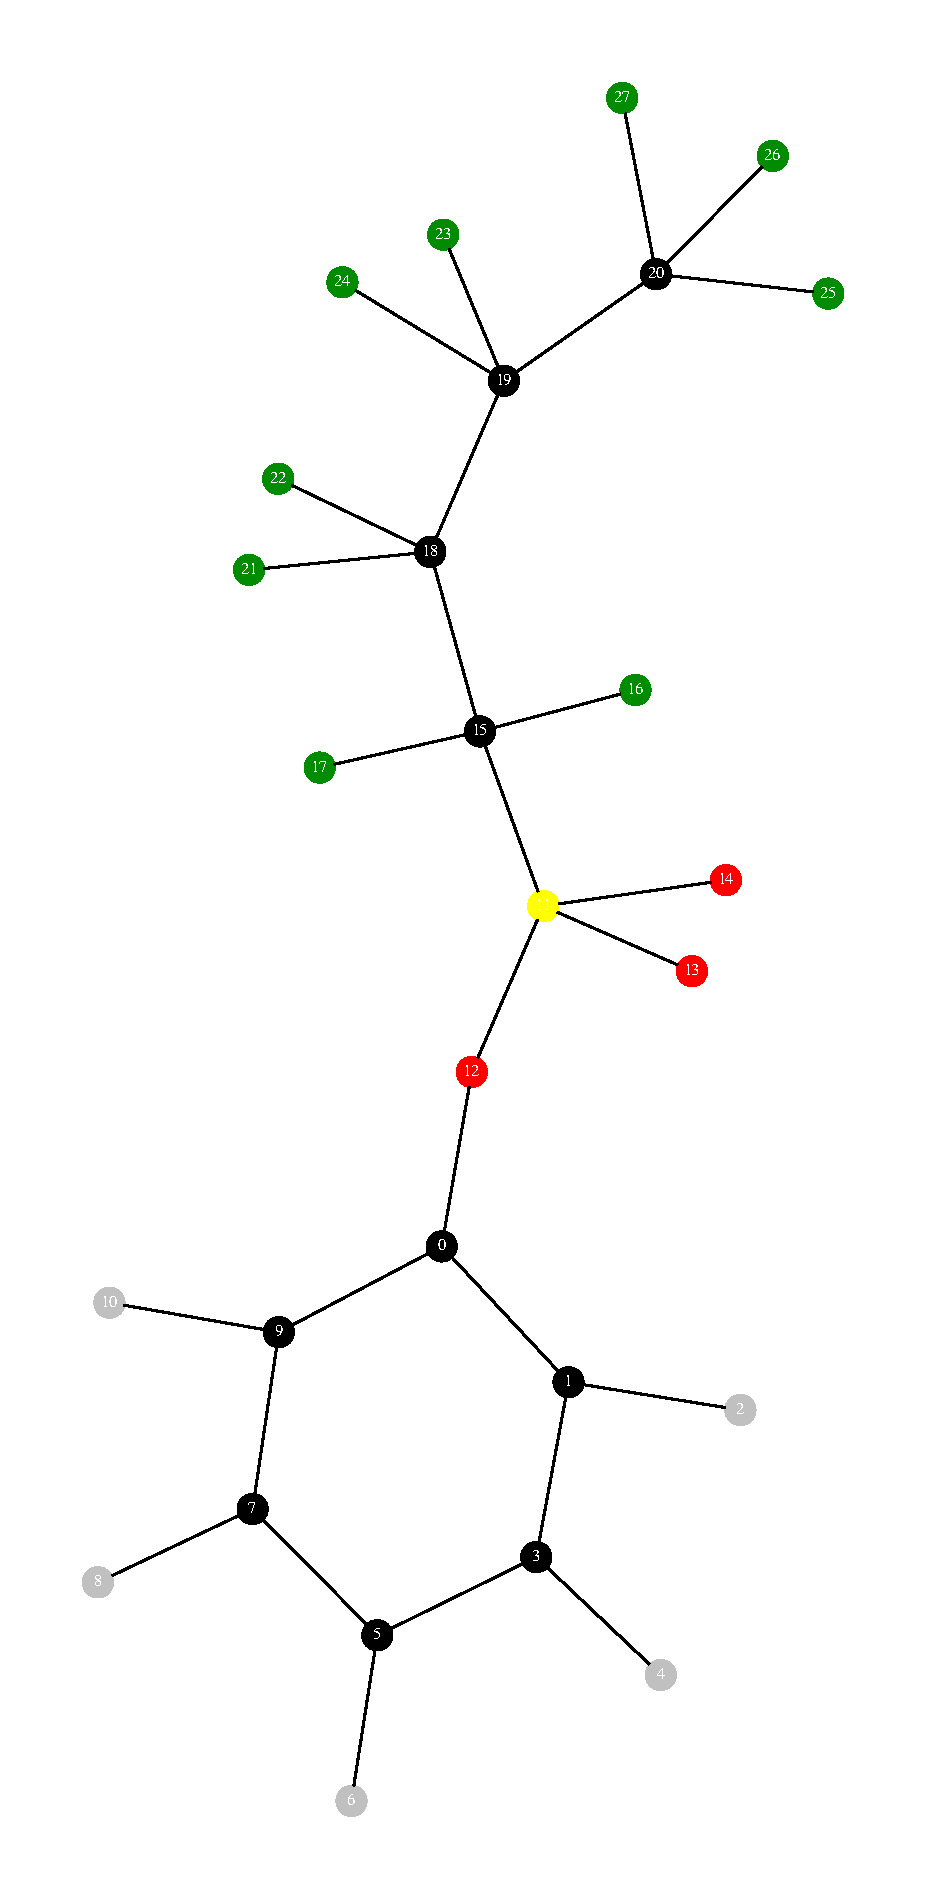
\includegraphics[scale=0.15]{mol_pictures_unfiltered/0.pdf}}

\vspace{1cm}
\begin{verbatim}
<HiPRGen.species_questions.species_default_true object at 0x2b667d6b2430>
Terminal.KEEP
\end{verbatim}


number: 1



entry id: af0733dcda4cc3494970c99618faad2a-C4H9O1-m1-1



uncorrected free energy: -6340.551332453043



formula: C4 H9 O1

\raisebox{-.5\height}{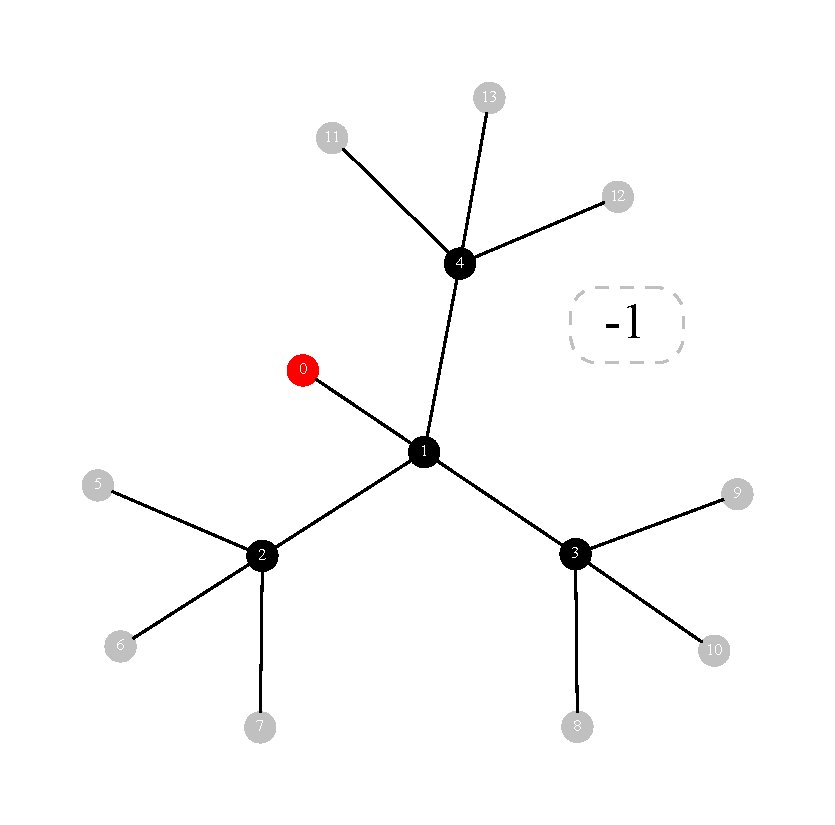
\includegraphics[scale=0.15]{mol_pictures_unfiltered/1.pdf}}

\vspace{1cm}
\begin{verbatim}
<HiPRGen.species_questions.species_default_true object at 0x2b667d6b2430>
Terminal.KEEP
\end{verbatim}


number: 2



entry id: 22ad4d4343667554c075f68e93c5c419-C4H9O1-0-2



uncorrected free energy: -6337.038072173203



formula: C4 H9 O1

\raisebox{-.5\height}{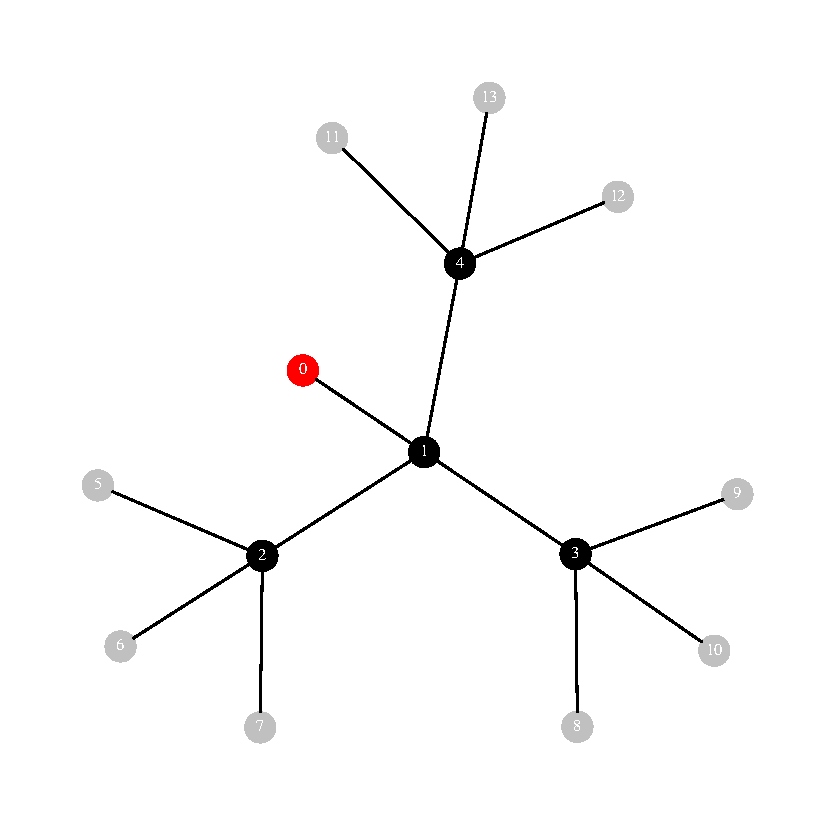
\includegraphics[scale=0.15]{mol_pictures_unfiltered/2.pdf}}

\vspace{1cm}
\begin{verbatim}
<HiPRGen.species_questions.species_default_true object at 0x2b667d6b2430>
Terminal.KEEP
\end{verbatim}


number: 3



entry id: db346580544213066bb82c346b1fff3a-C12H10S1-m1-2



uncorrected free energy: -23437.70611996324



formula: C12 H10 S1

\raisebox{-.5\height}{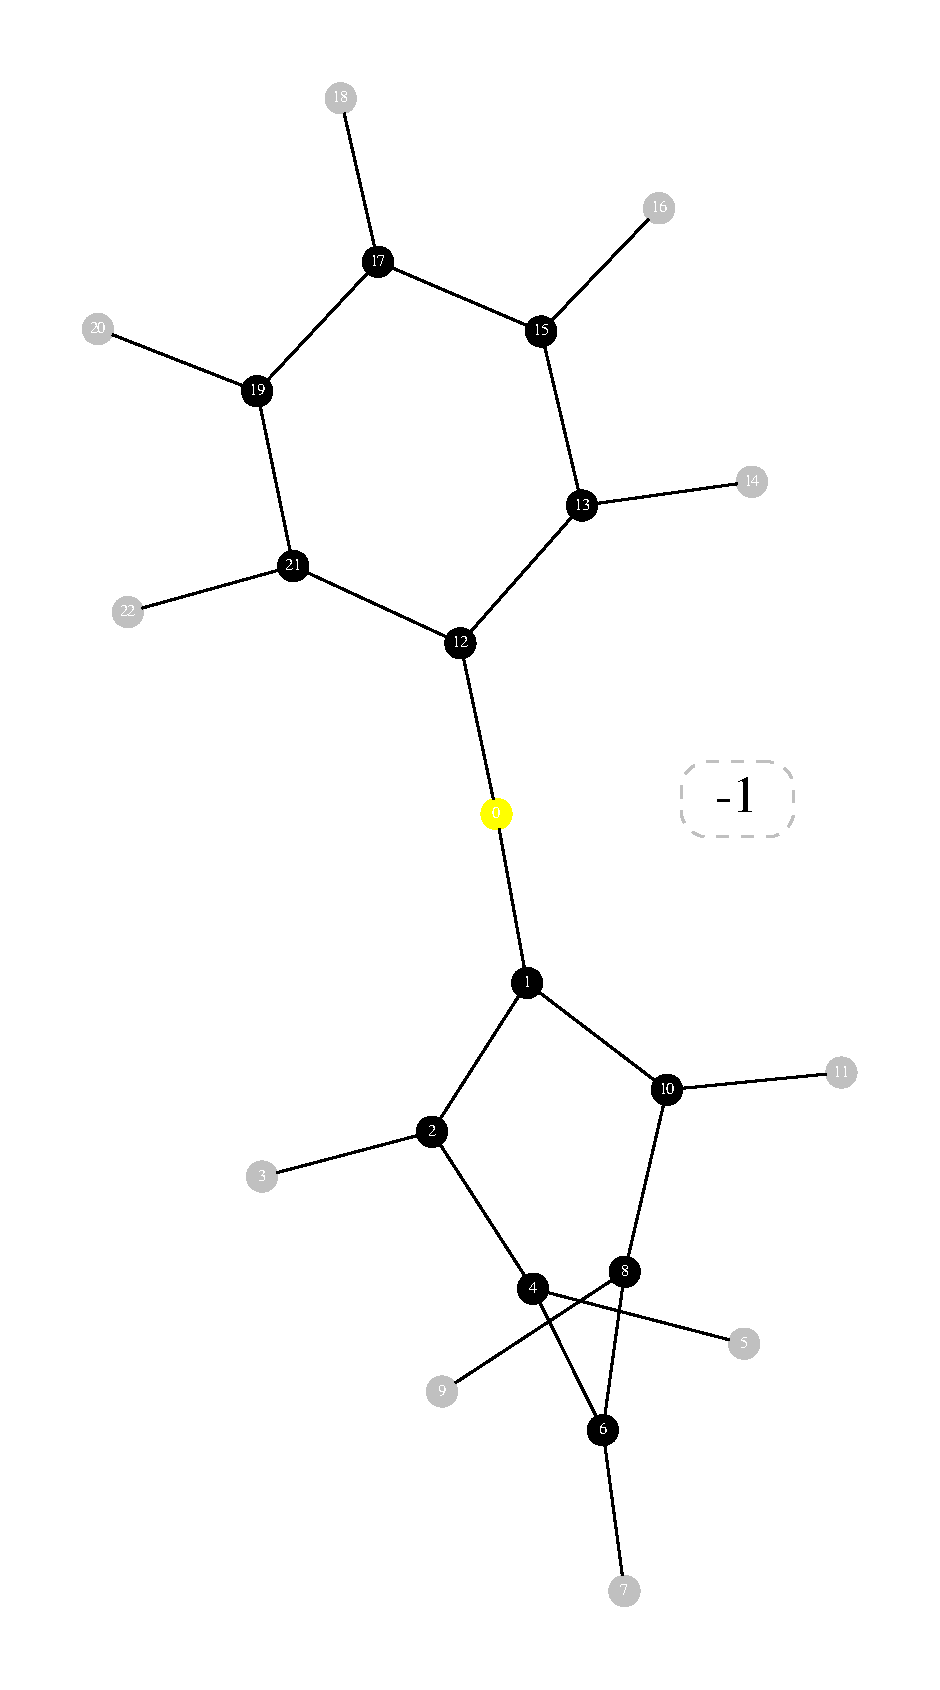
\includegraphics[scale=0.15]{mol_pictures_unfiltered/3.pdf}}

\vspace{1cm}
\begin{verbatim}
<HiPRGen.species_questions.species_default_true object at 0x2b667d6b2430>
Terminal.KEEP
\end{verbatim}


number: 4



entry id: bc3641376a32020a0345549009577712-C12H10S1-0-1



uncorrected free energy: -23437.039385831296



formula: C12 H10 S1

\raisebox{-.5\height}{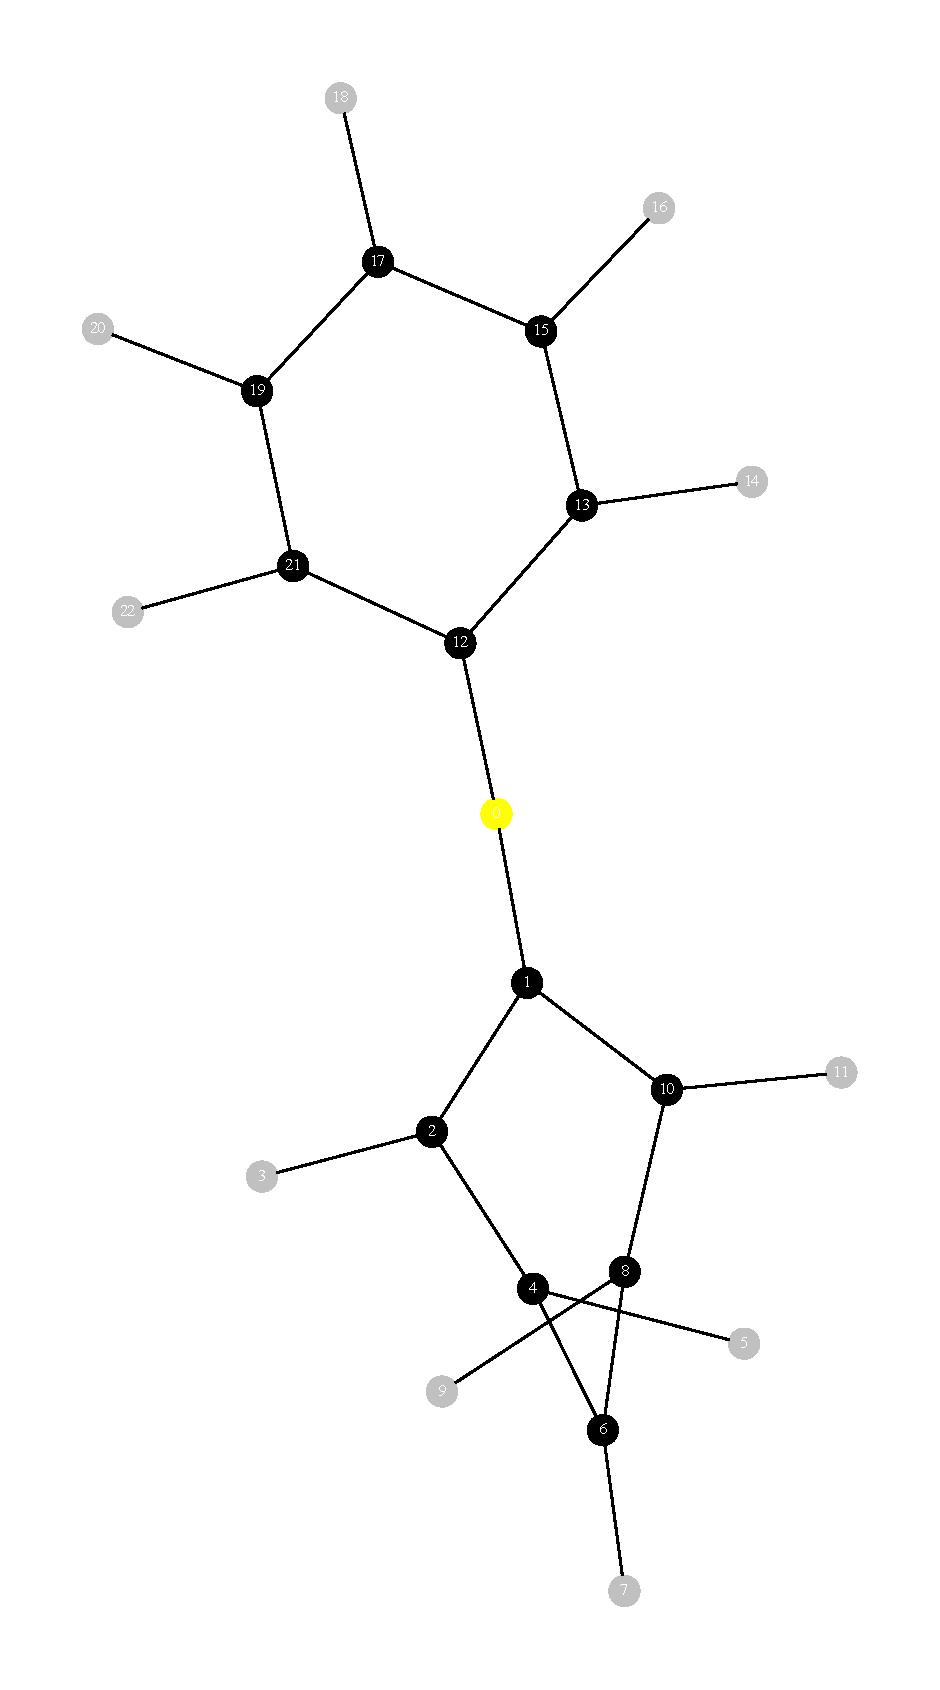
\includegraphics[scale=0.15]{mol_pictures_unfiltered/4.pdf}}

\vspace{1cm}
\begin{verbatim}
<HiPRGen.species_questions.species_default_true object at 0x2b667d6b2430>
Terminal.KEEP
\end{verbatim}


number: 5



entry id: e524cbadc1649d2535bdee66942e4dba-C12H10S1-1-2



uncorrected free energy: -23430.495352141443



formula: C12 H10 S1

\raisebox{-.5\height}{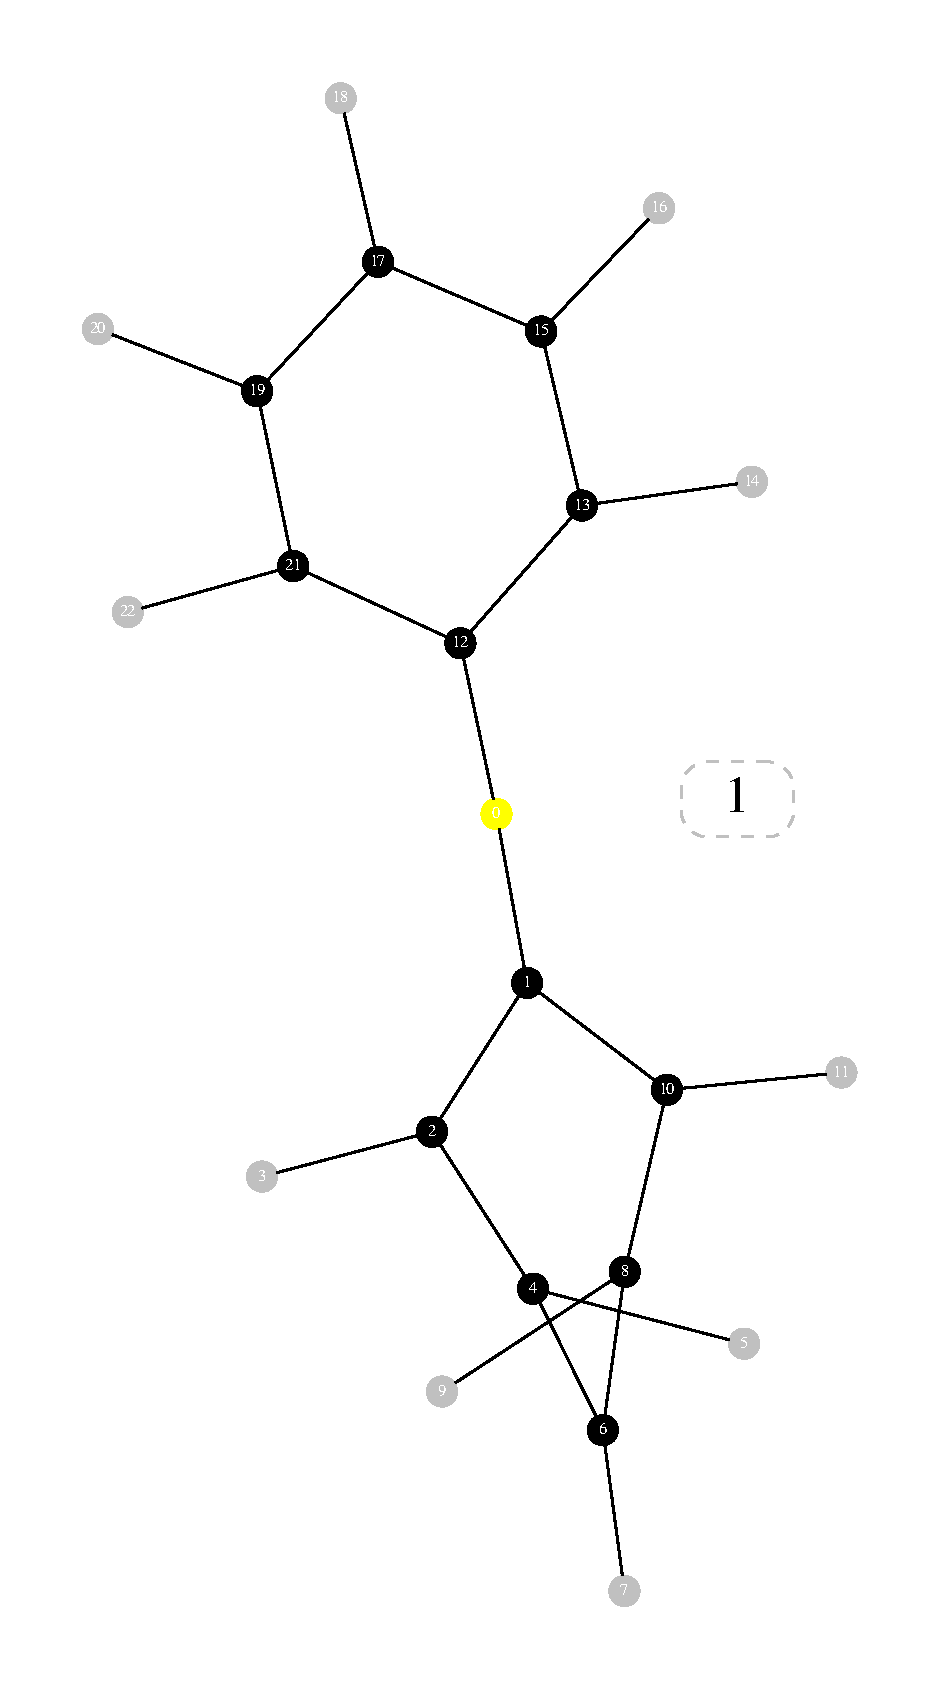
\includegraphics[scale=0.15]{mol_pictures_unfiltered/5.pdf}}

\vspace{1cm}
\begin{verbatim}
<HiPRGen.species_questions.species_default_true object at 0x2b667d6b2430>
Terminal.KEEP
\end{verbatim}


number: 6



entry id: ebf68aa2f6d4a07641dcb570486ea86d-O3S1-m2-1



uncorrected free energy: -16981.496435199475



formula: O3 S1

\raisebox{-.5\height}{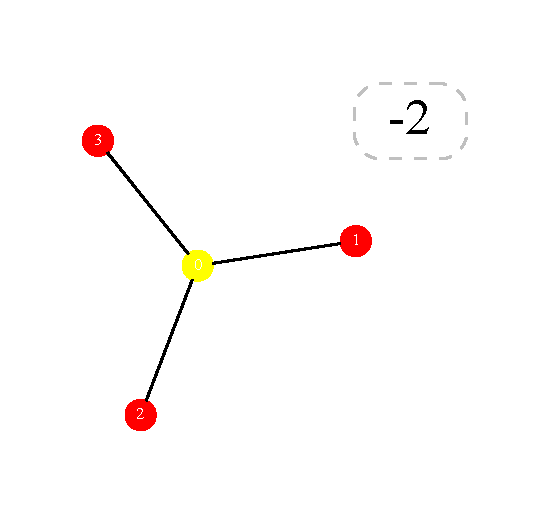
\includegraphics[scale=0.15]{mol_pictures_unfiltered/6.pdf}}

\vspace{1cm}
\begin{verbatim}
<HiPRGen.species_questions.species_default_true object at 0x2b667d6b2430>
Terminal.KEEP
\end{verbatim}


number: 7



entry id: 4fae9656fce777fe31f204f123fa4921-O3S1-m1-2



uncorrected free energy: -16980.038738980504



formula: O3 S1

\raisebox{-.5\height}{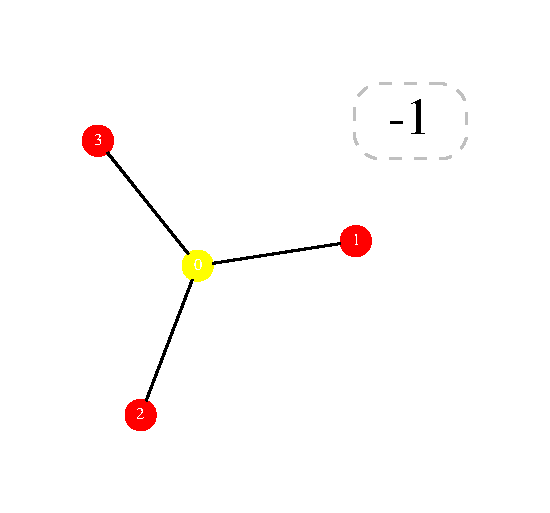
\includegraphics[scale=0.15]{mol_pictures_unfiltered/7.pdf}}

\vspace{1cm}
\begin{verbatim}
<HiPRGen.species_questions.species_default_true object at 0x2b667d6b2430>
Terminal.KEEP
\end{verbatim}


number: 8



entry id: 06ec8edf4209e7e492b8e563b71afbeb-O3S1-0-1



uncorrected free energy: -16976.242933424644



formula: O3 S1

\raisebox{-.5\height}{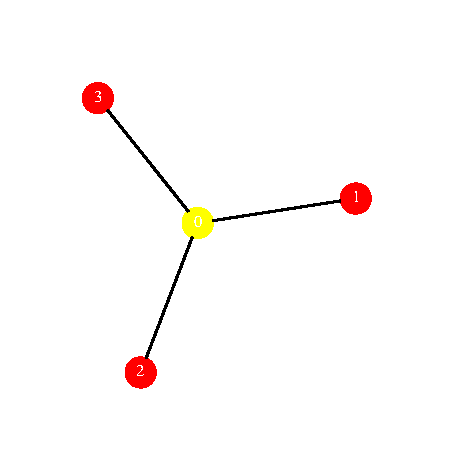
\includegraphics[scale=0.15]{mol_pictures_unfiltered/8.pdf}}

\vspace{1cm}
\begin{verbatim}
<HiPRGen.species_questions.species_default_true object at 0x2b667d6b2430>
Terminal.KEEP
\end{verbatim}


number: 9



entry id: 9100204becf2990b58581af65fd3b696-O3S1-1-2



uncorrected free energy: -16965.25336250728



formula: O3 S1

\raisebox{-.5\height}{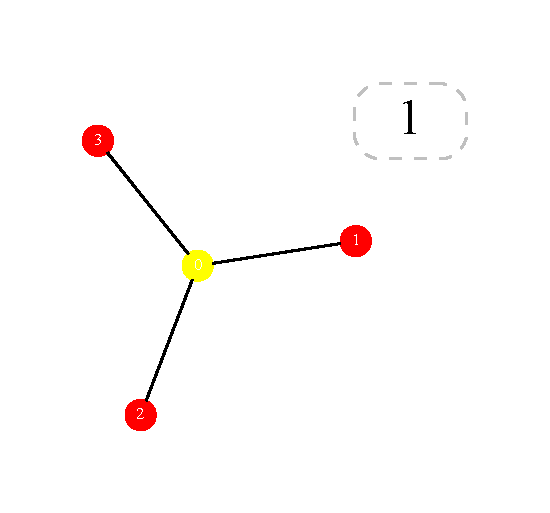
\includegraphics[scale=0.15]{mol_pictures_unfiltered/9.pdf}}

\vspace{1cm}
\begin{verbatim}
<HiPRGen.species_questions.species_default_true object at 0x2b667d6b2430>
Terminal.KEEP
\end{verbatim}


number: 10



entry id: ce02829e6764a1bba90ddba3eabc3c6a-C15H28O4-m1-2



uncorrected free energy: -24191.628919694365



formula: C15 H28 O4

\raisebox{-.5\height}{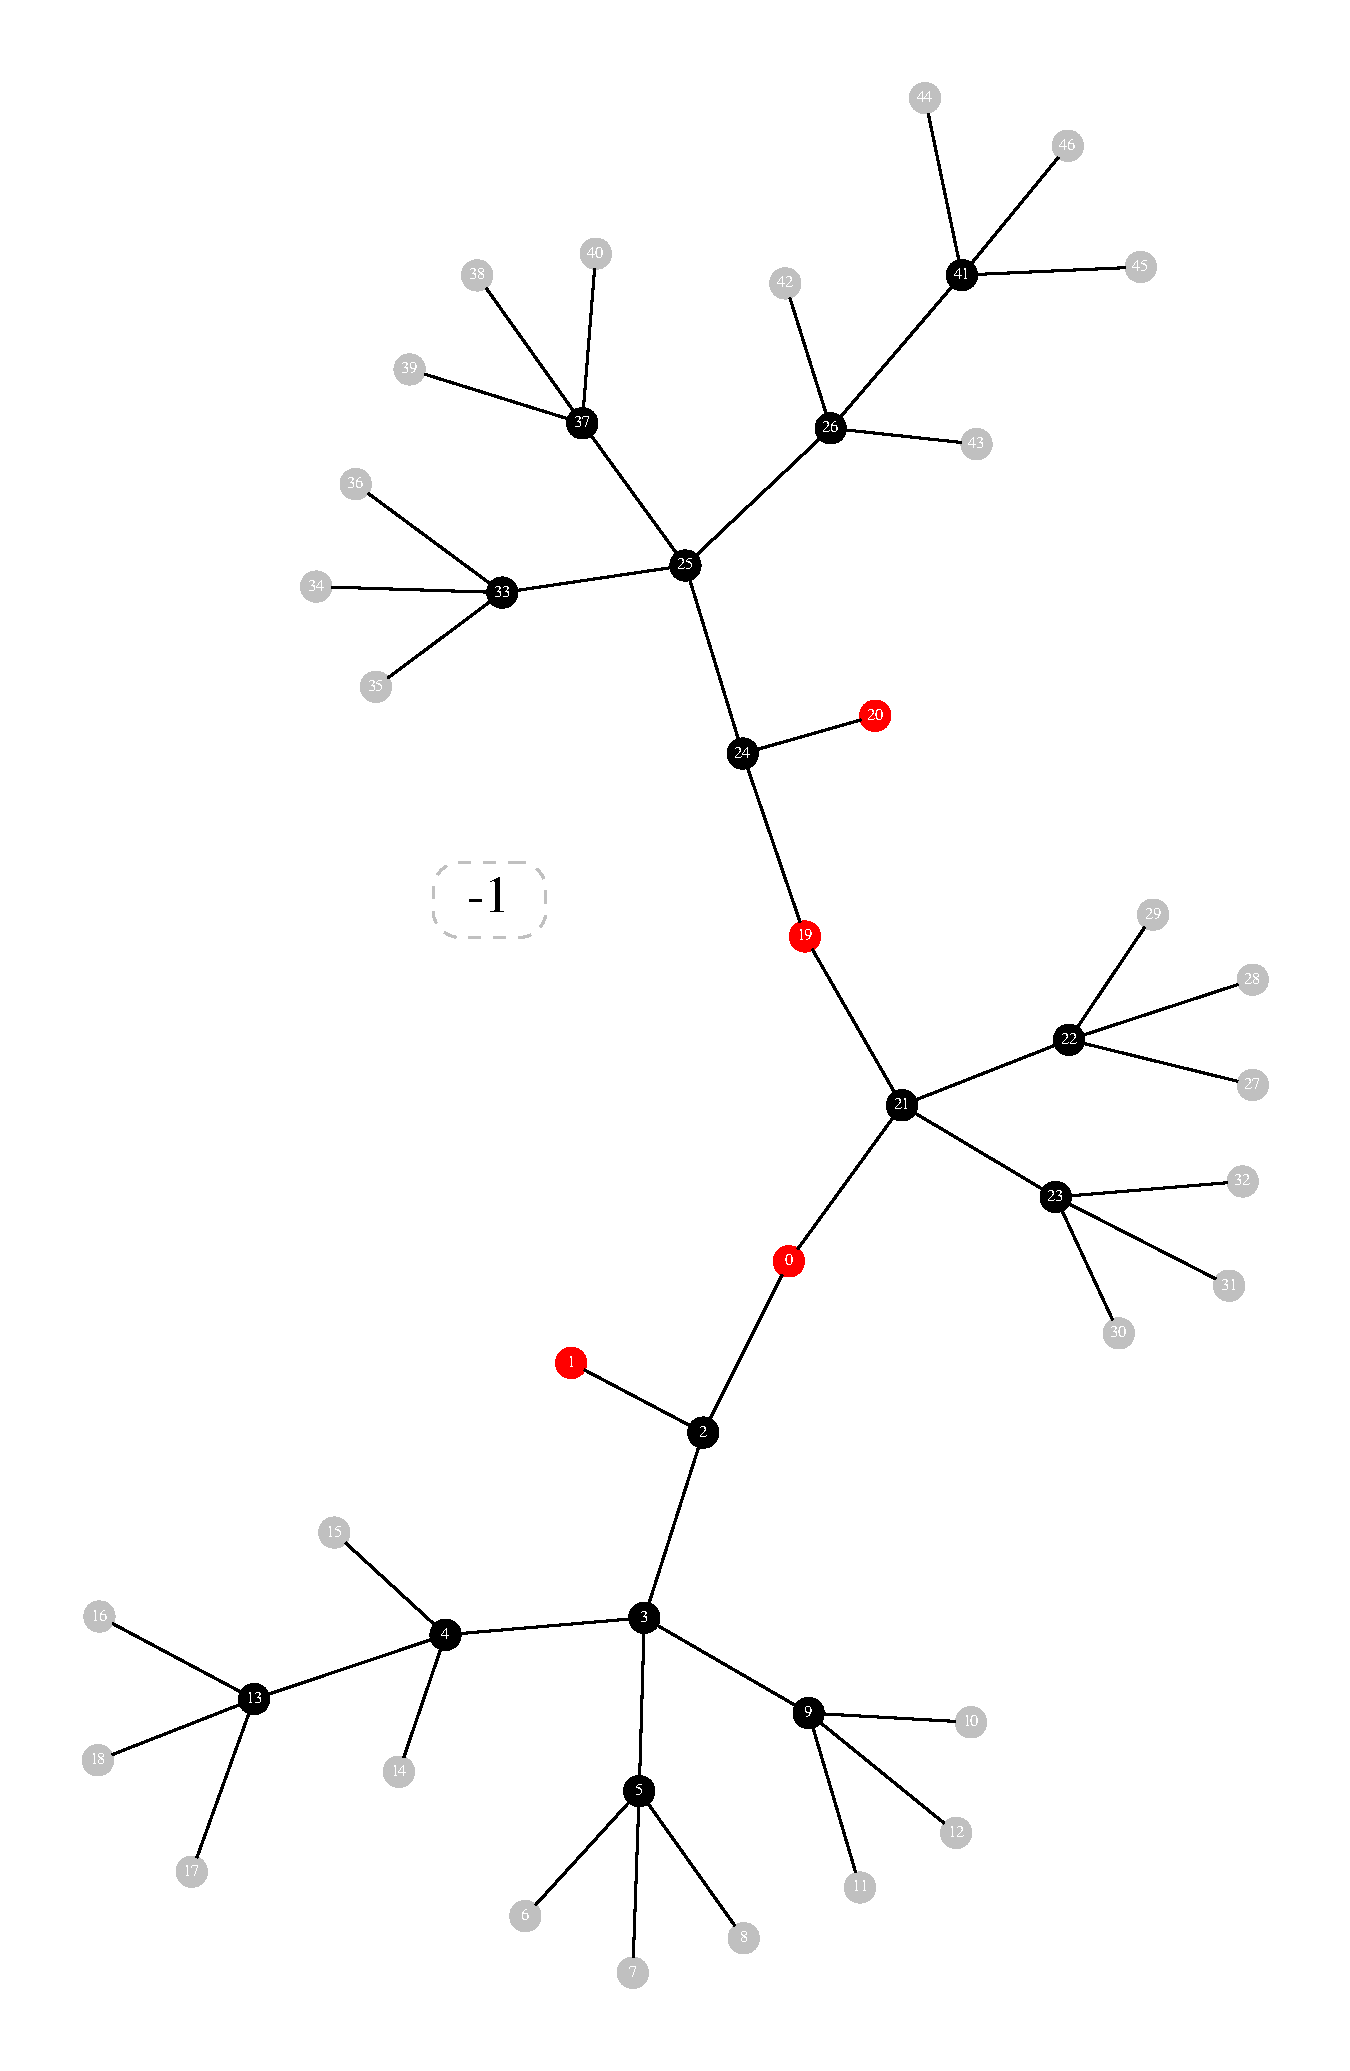
\includegraphics[scale=0.15]{mol_pictures_unfiltered/10.pdf}}

\vspace{1cm}
\begin{verbatim}
<HiPRGen.species_questions.species_default_true object at 0x2b667d6b2430>
Terminal.KEEP
\end{verbatim}


number: 11



entry id: affe6041ffe648433daa714b2d39dd72-C15H28O4-0-1



uncorrected free energy: -24191.05630934911



formula: C15 H28 O4

\raisebox{-.5\height}{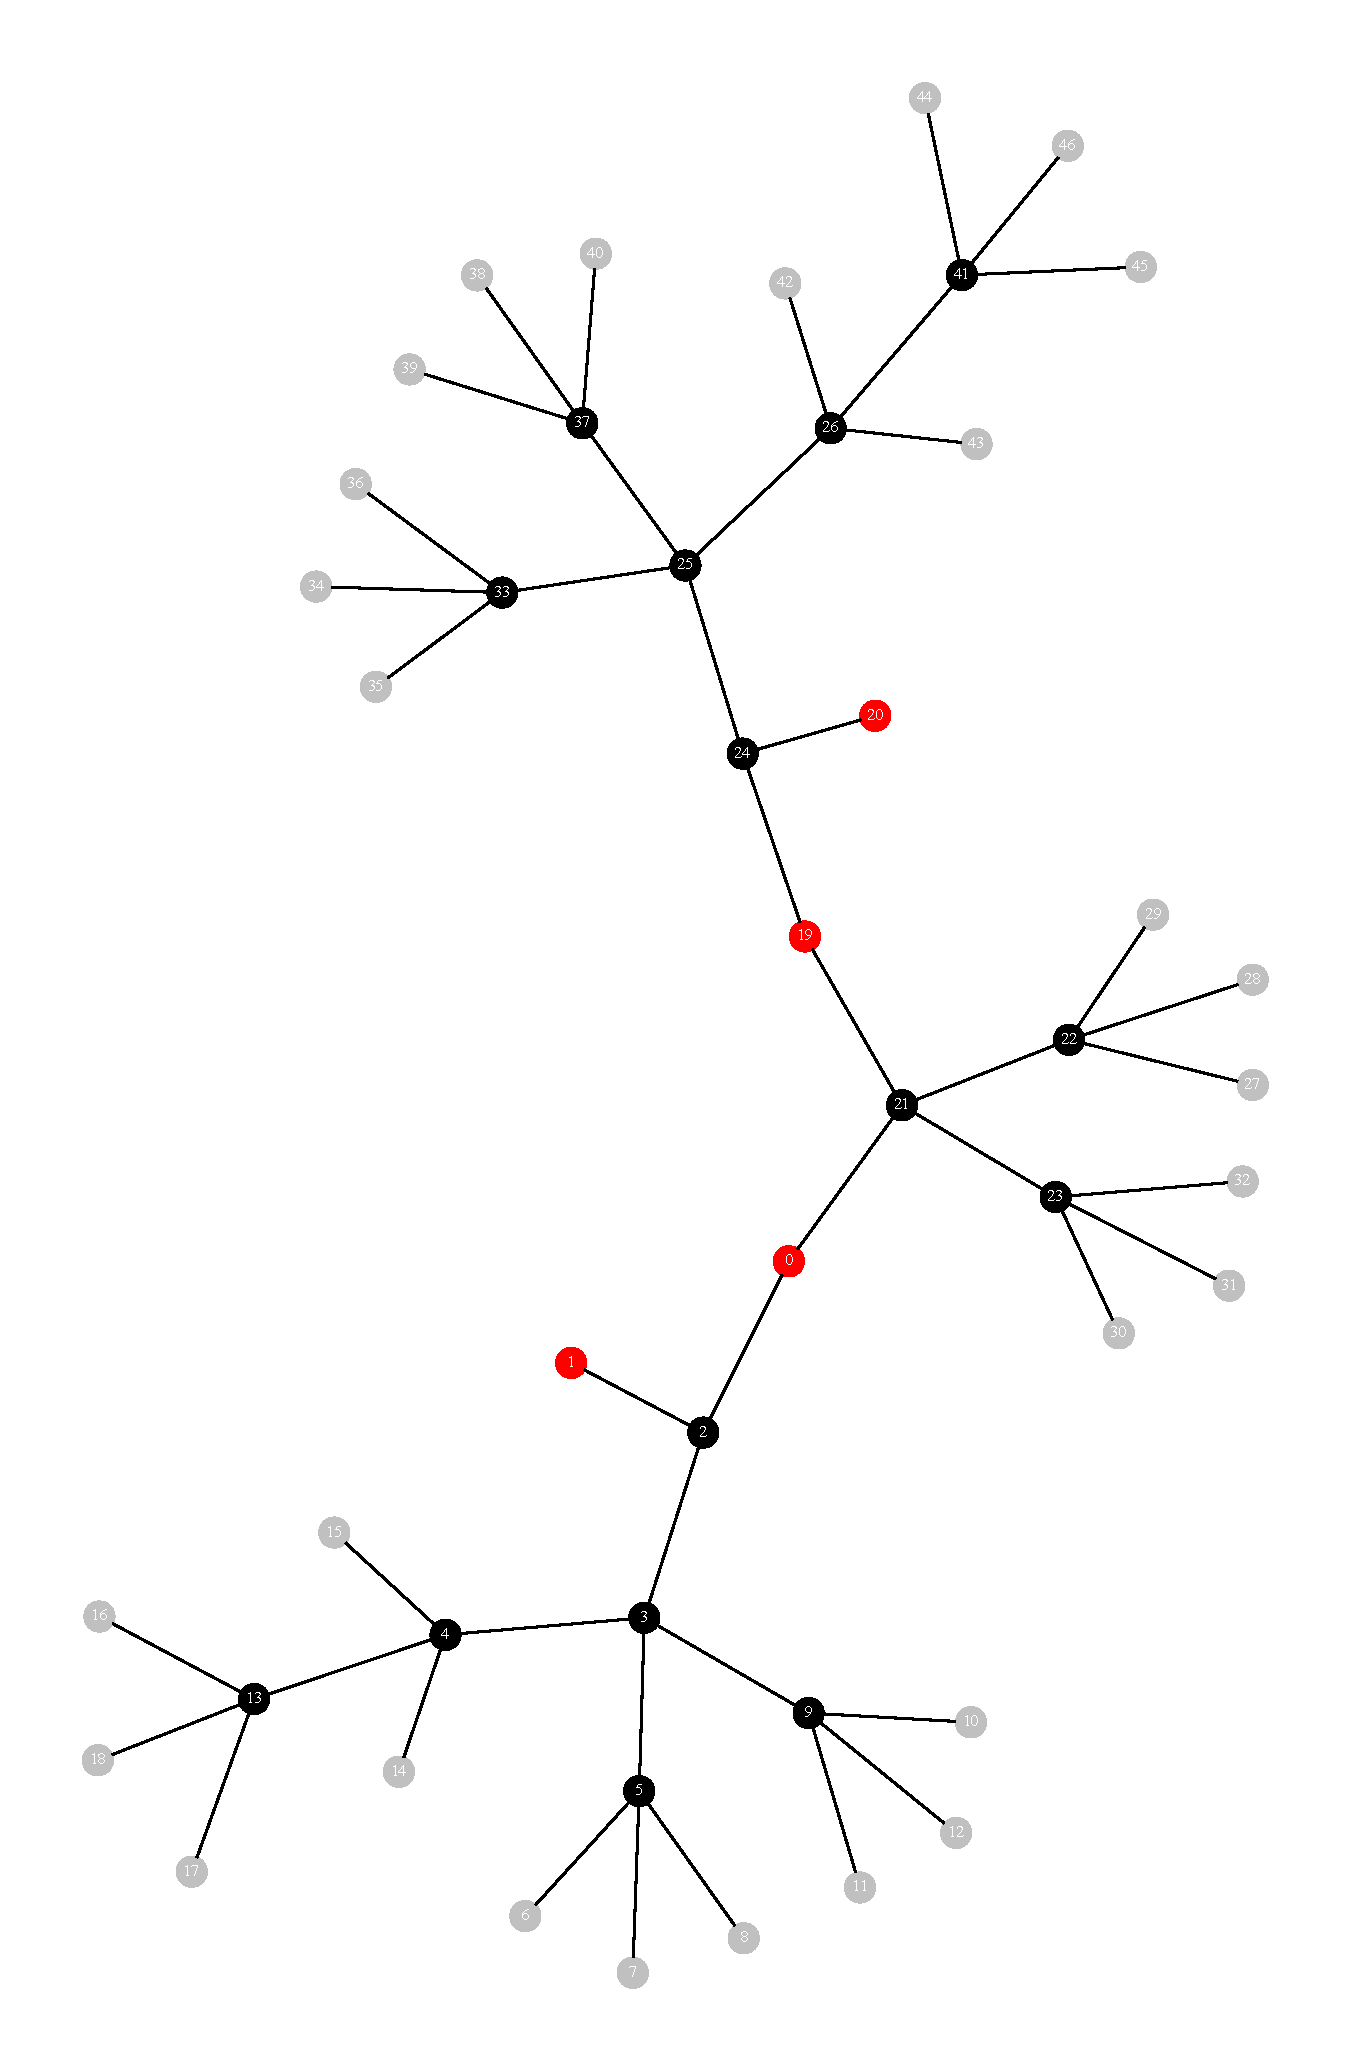
\includegraphics[scale=0.15]{mol_pictures_unfiltered/11.pdf}}

\vspace{1cm}
\begin{verbatim}
<HiPRGen.species_questions.species_default_true object at 0x2b667d6b2430>
Terminal.KEEP
\end{verbatim}


number: 12



entry id: 8425c6cfd18e1596203ba12ba792a30e-C15H28O4-1-2



uncorrected free energy: -24182.736968514186



formula: C15 H28 O4

\raisebox{-.5\height}{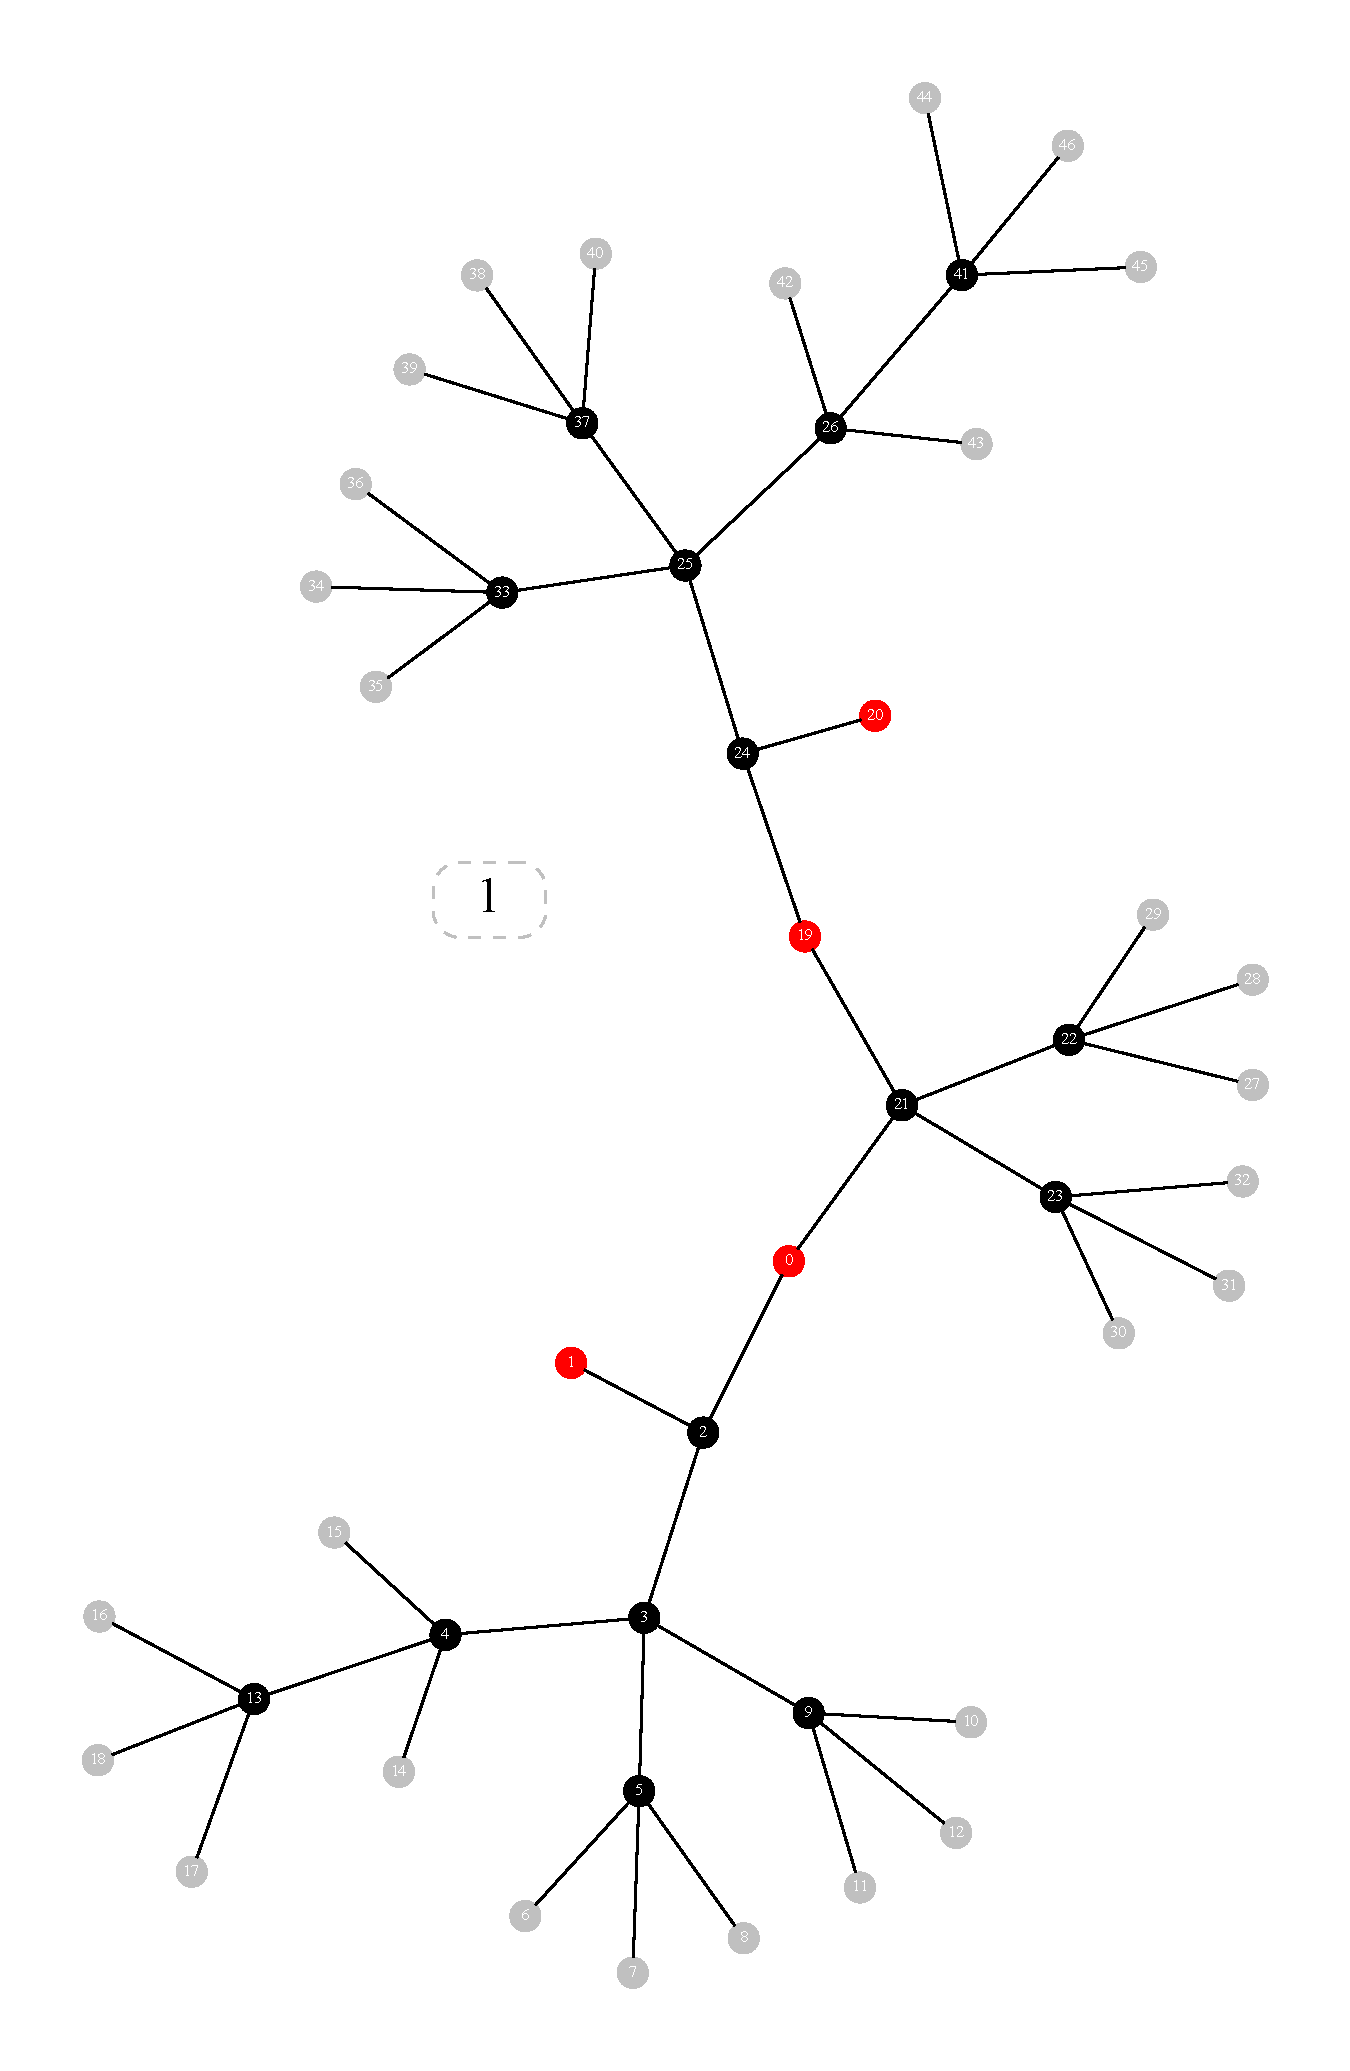
\includegraphics[scale=0.15]{mol_pictures_unfiltered/12.pdf}}

\vspace{1cm}
\begin{verbatim}
<HiPRGen.species_questions.species_default_true object at 0x2b667d6b2430>
Terminal.KEEP
\end{verbatim}


number: 13



entry id: 89f973ce0822f0ba97d90b7b4377454f-C10H21O2-m1-1



uncorrected free energy: -14799.207919582419



formula: C10 H21 O2

\raisebox{-.5\height}{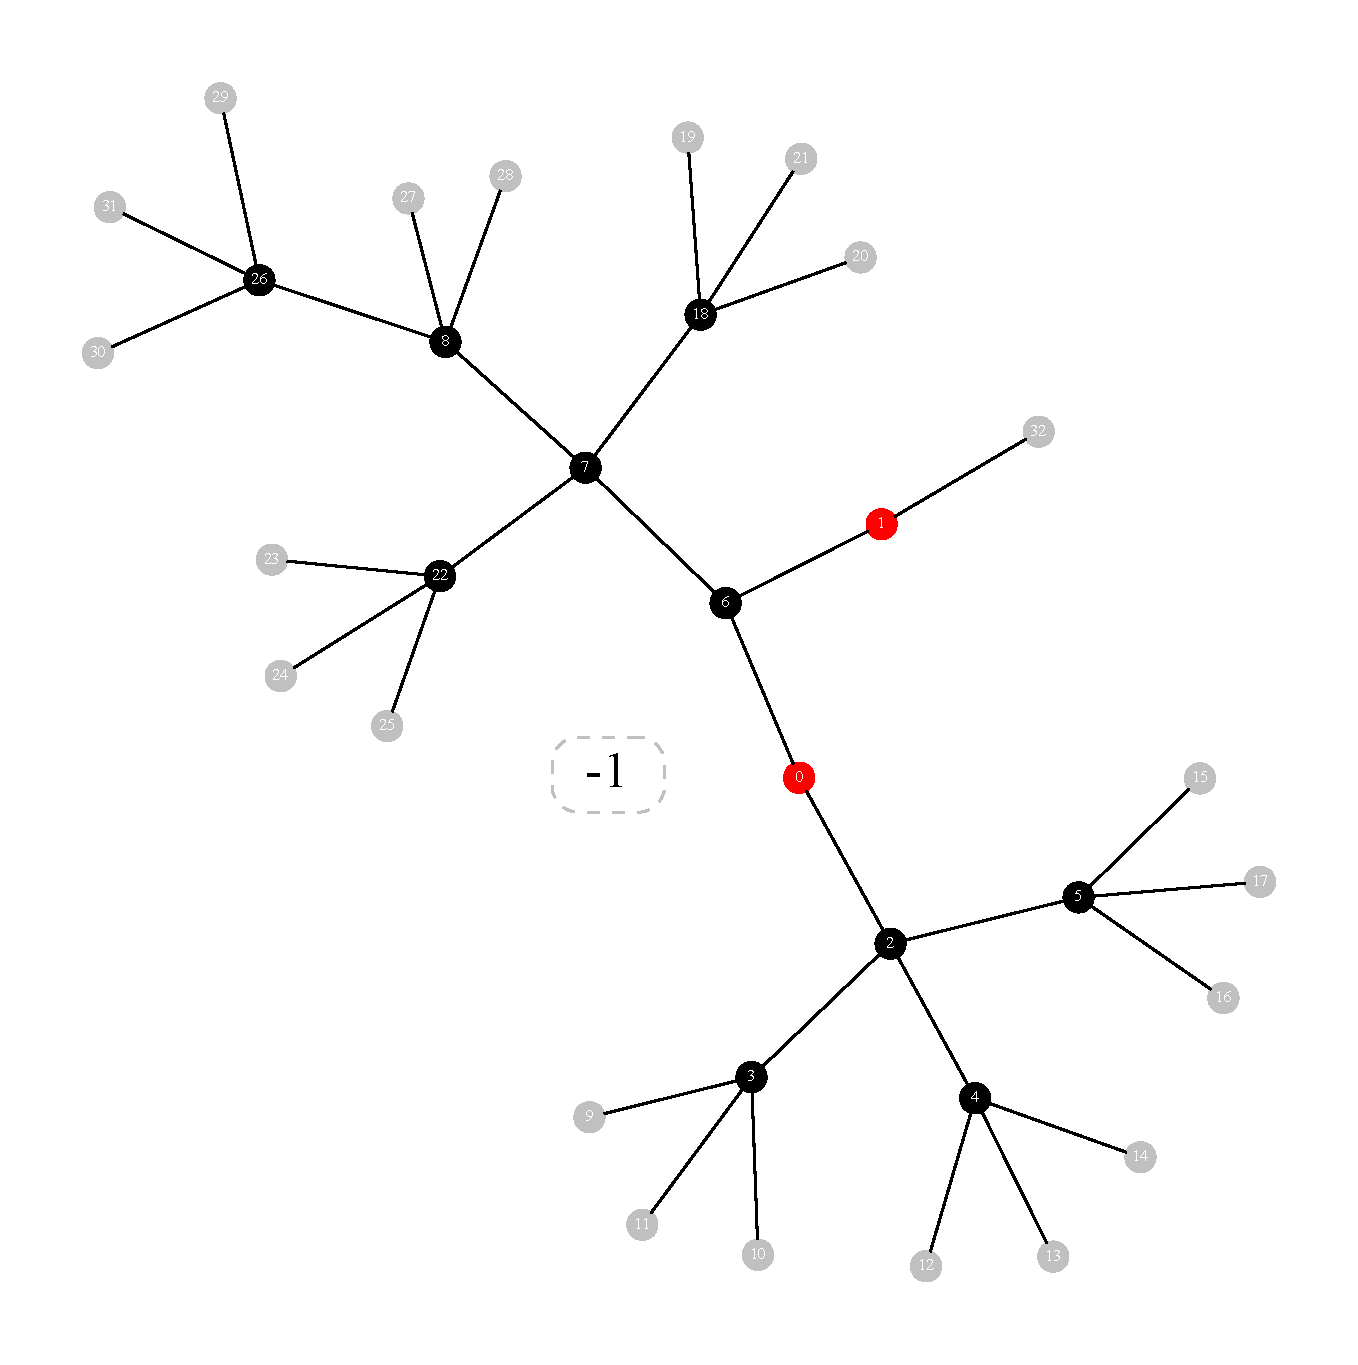
\includegraphics[scale=0.15]{mol_pictures_unfiltered/13.pdf}}

\vspace{1cm}
\begin{verbatim}
<HiPRGen.species_questions.species_default_true object at 0x2b667d6b2430>
Terminal.KEEP
\end{verbatim}


number: 14



entry id: 8a7e8693a6998655afc6c3cd13715281-C10H21O2-0-2



uncorrected free energy: -14797.527224036618



formula: C10 H21 O2

\raisebox{-.5\height}{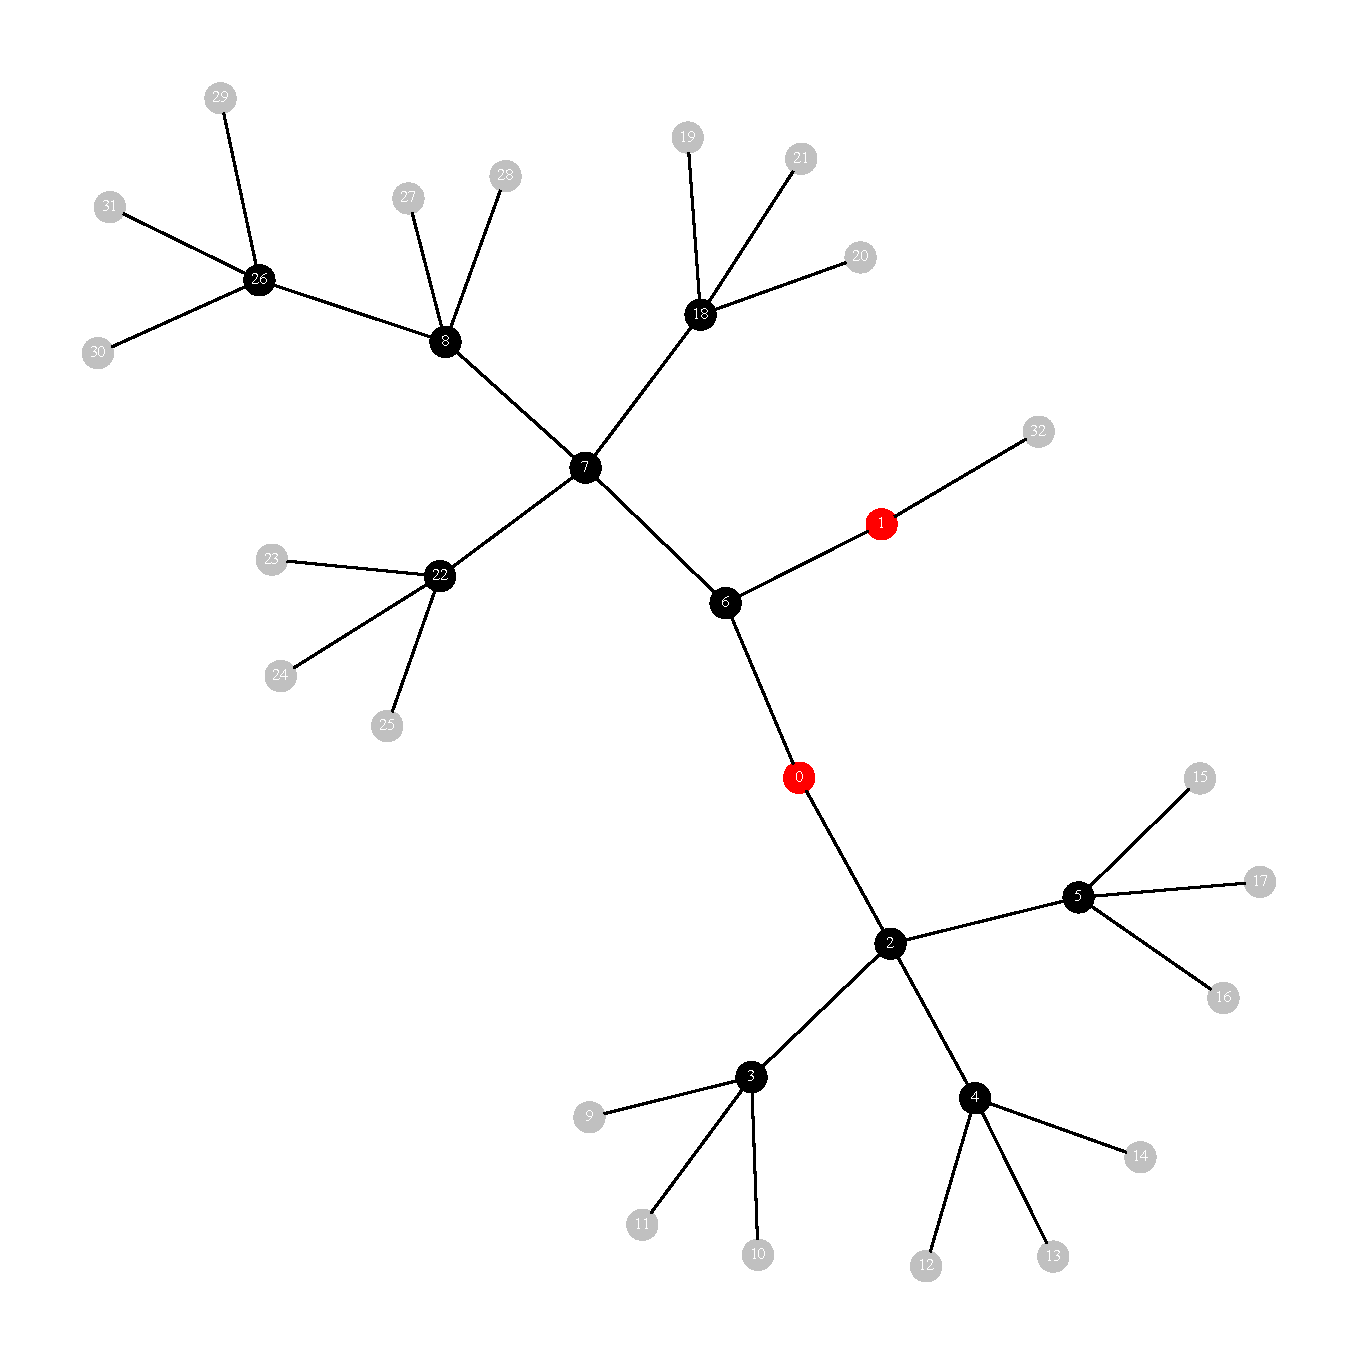
\includegraphics[scale=0.15]{mol_pictures_unfiltered/14.pdf}}

\vspace{1cm}
\begin{verbatim}
<HiPRGen.species_questions.species_default_true object at 0x2b667d6b2430>
Terminal.KEEP
\end{verbatim}


number: 15



entry id: 2c137c7f62959d051173f4c02a854944-C10H21O2-1-1



uncorrected free energy: -14793.836633812178



formula: C10 H21 O2

\raisebox{-.5\height}{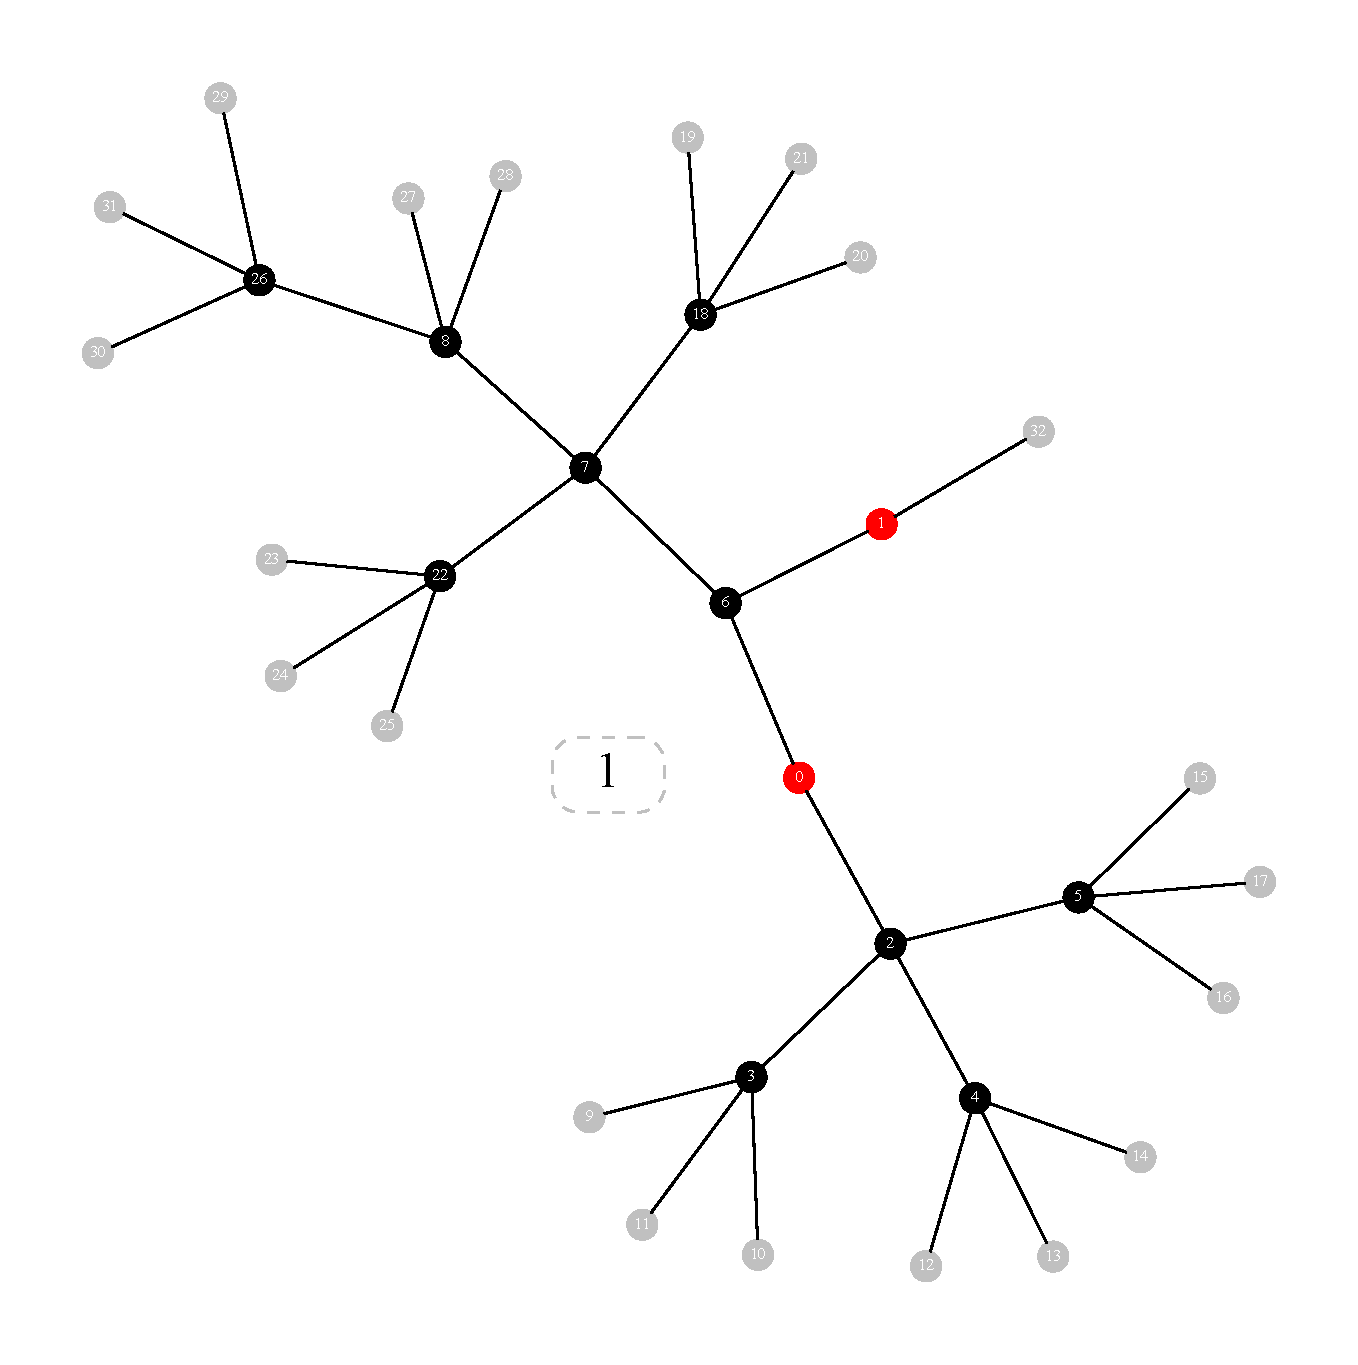
\includegraphics[scale=0.15]{mol_pictures_unfiltered/15.pdf}}

\vspace{1cm}
\begin{verbatim}
<HiPRGen.species_questions.species_default_true object at 0x2b667d6b2430>
Terminal.KEEP
\end{verbatim}


number: 16



entry id: 2f65c8c819c26044f8a1b94755ad77b1-C12H11S1-1-1



uncorrected free energy: -23446.885503395588



formula: C12 H11 S1

\raisebox{-.5\height}{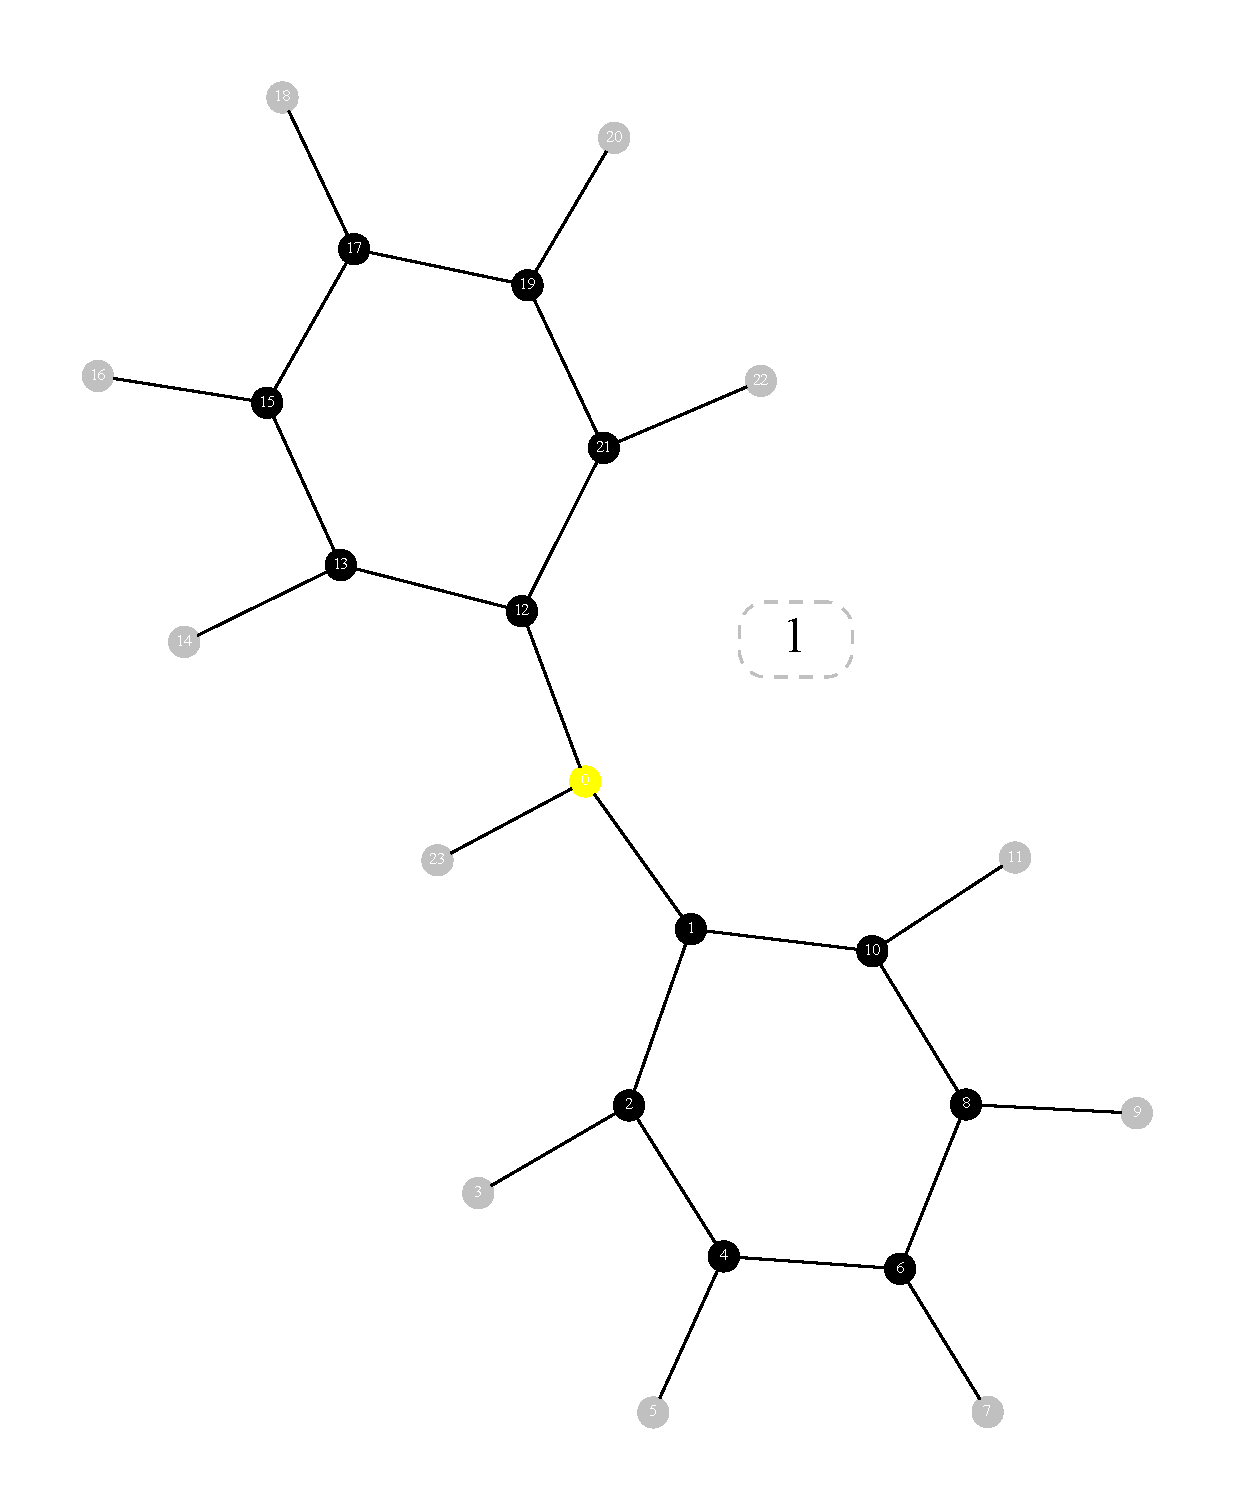
\includegraphics[scale=0.15]{mol_pictures_unfiltered/16.pdf}}

\vspace{1cm}
\begin{verbatim}
<HiPRGen.species_questions.species_default_true object at 0x2b667d6b2430>
Terminal.KEEP
\end{verbatim}


number: 17



entry id: e51d163ce60f39a477fbac74bf153e6e-C18H14S1-m1-2



uncorrected free energy: -29720.276875044165



formula: C18 H14 S1

\raisebox{-.5\height}{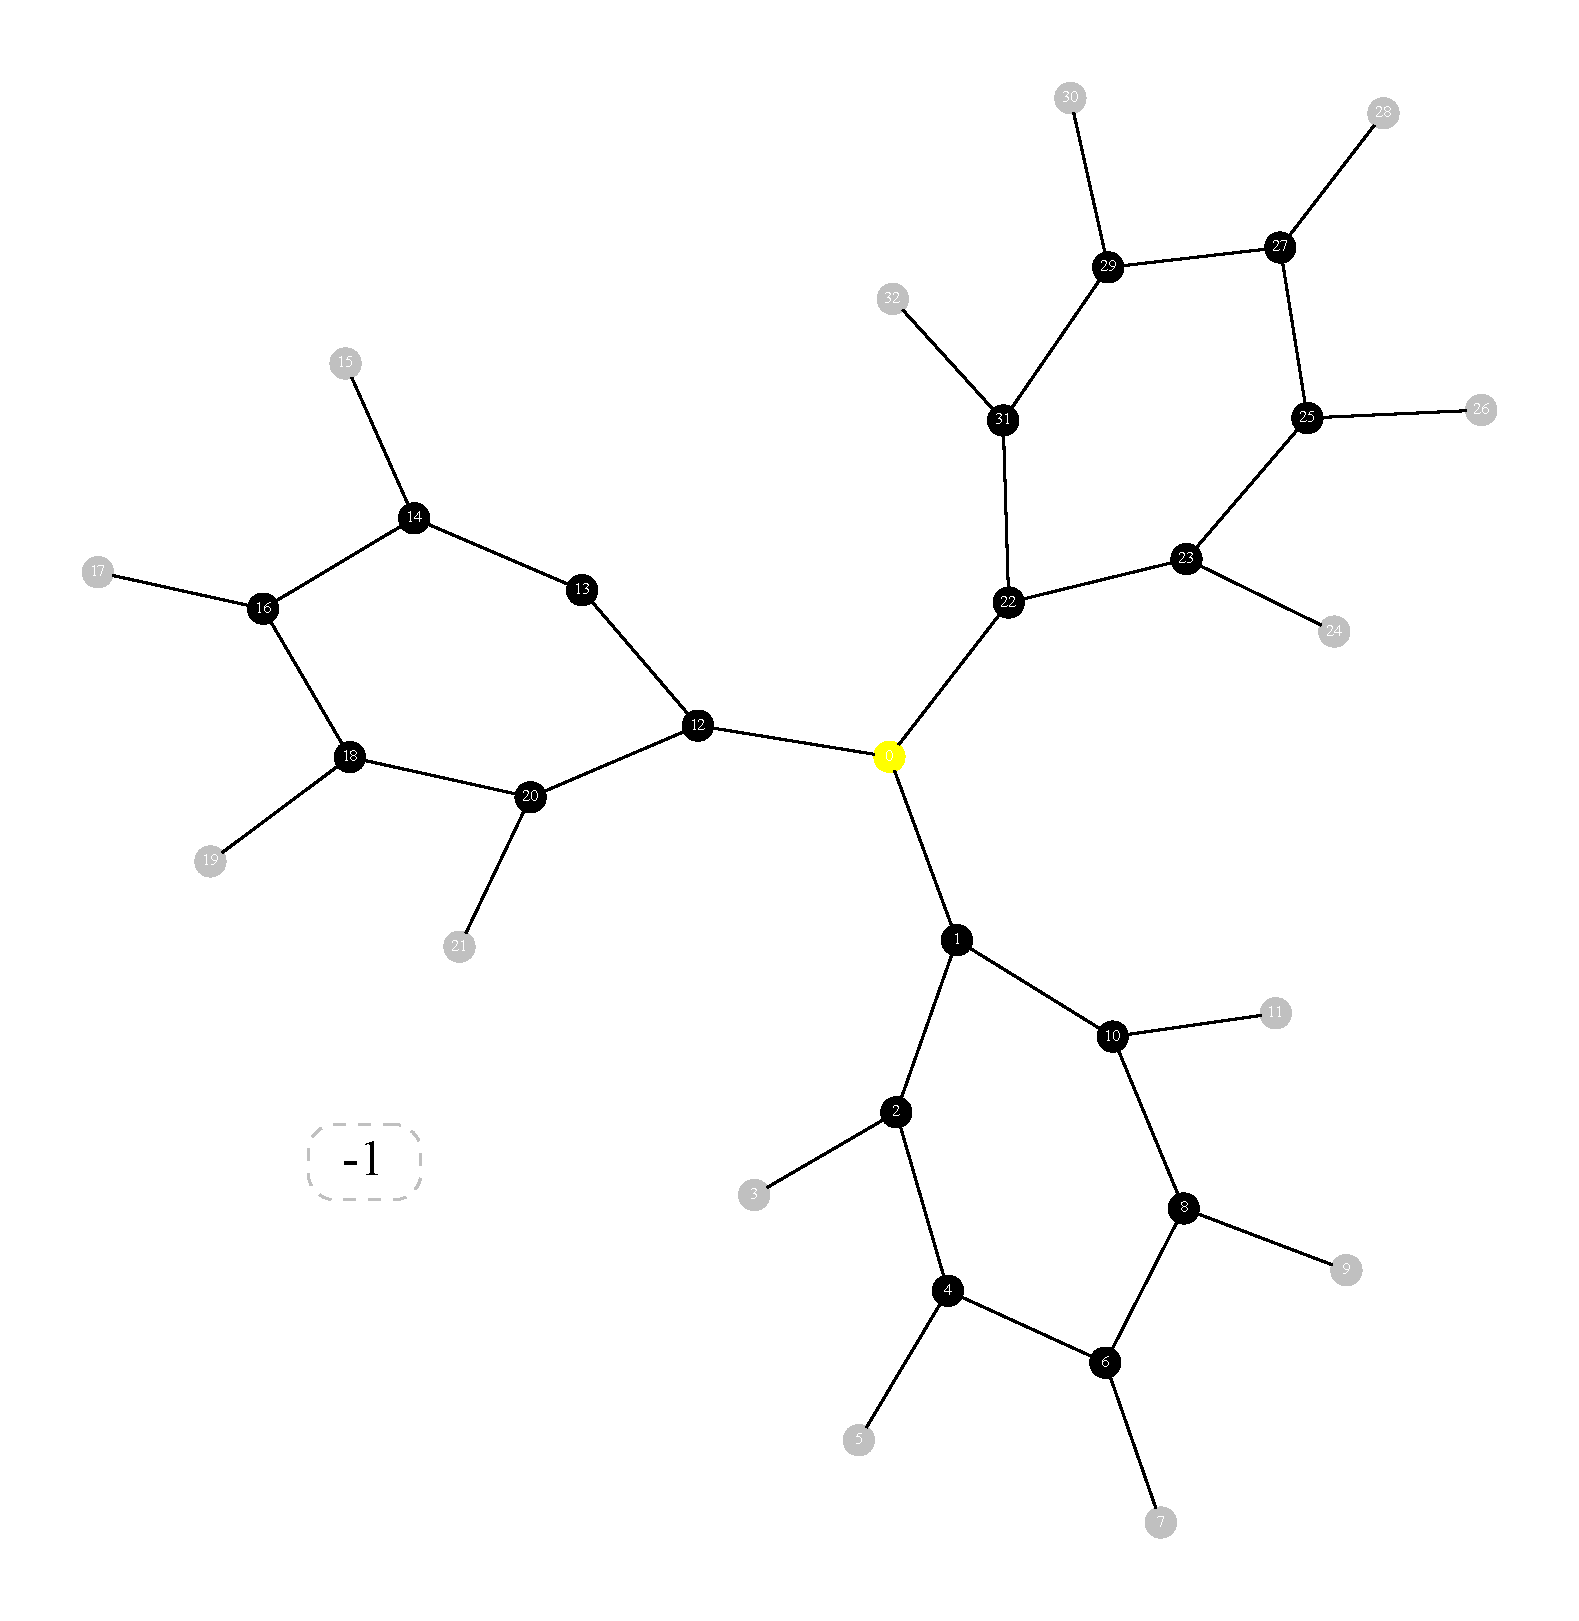
\includegraphics[scale=0.15]{mol_pictures_unfiltered/17.pdf}}

\vspace{1cm}
\begin{verbatim}
<HiPRGen.species_questions.species_default_true object at 0x2b667d6b2430>
Terminal.KEEP
\end{verbatim}


number: 18



entry id: d7c3b045b53266f82e25ae3098e29d4f-C18H14S1-0-1



uncorrected free energy: -29718.678399679367



formula: C18 H14 S1

\raisebox{-.5\height}{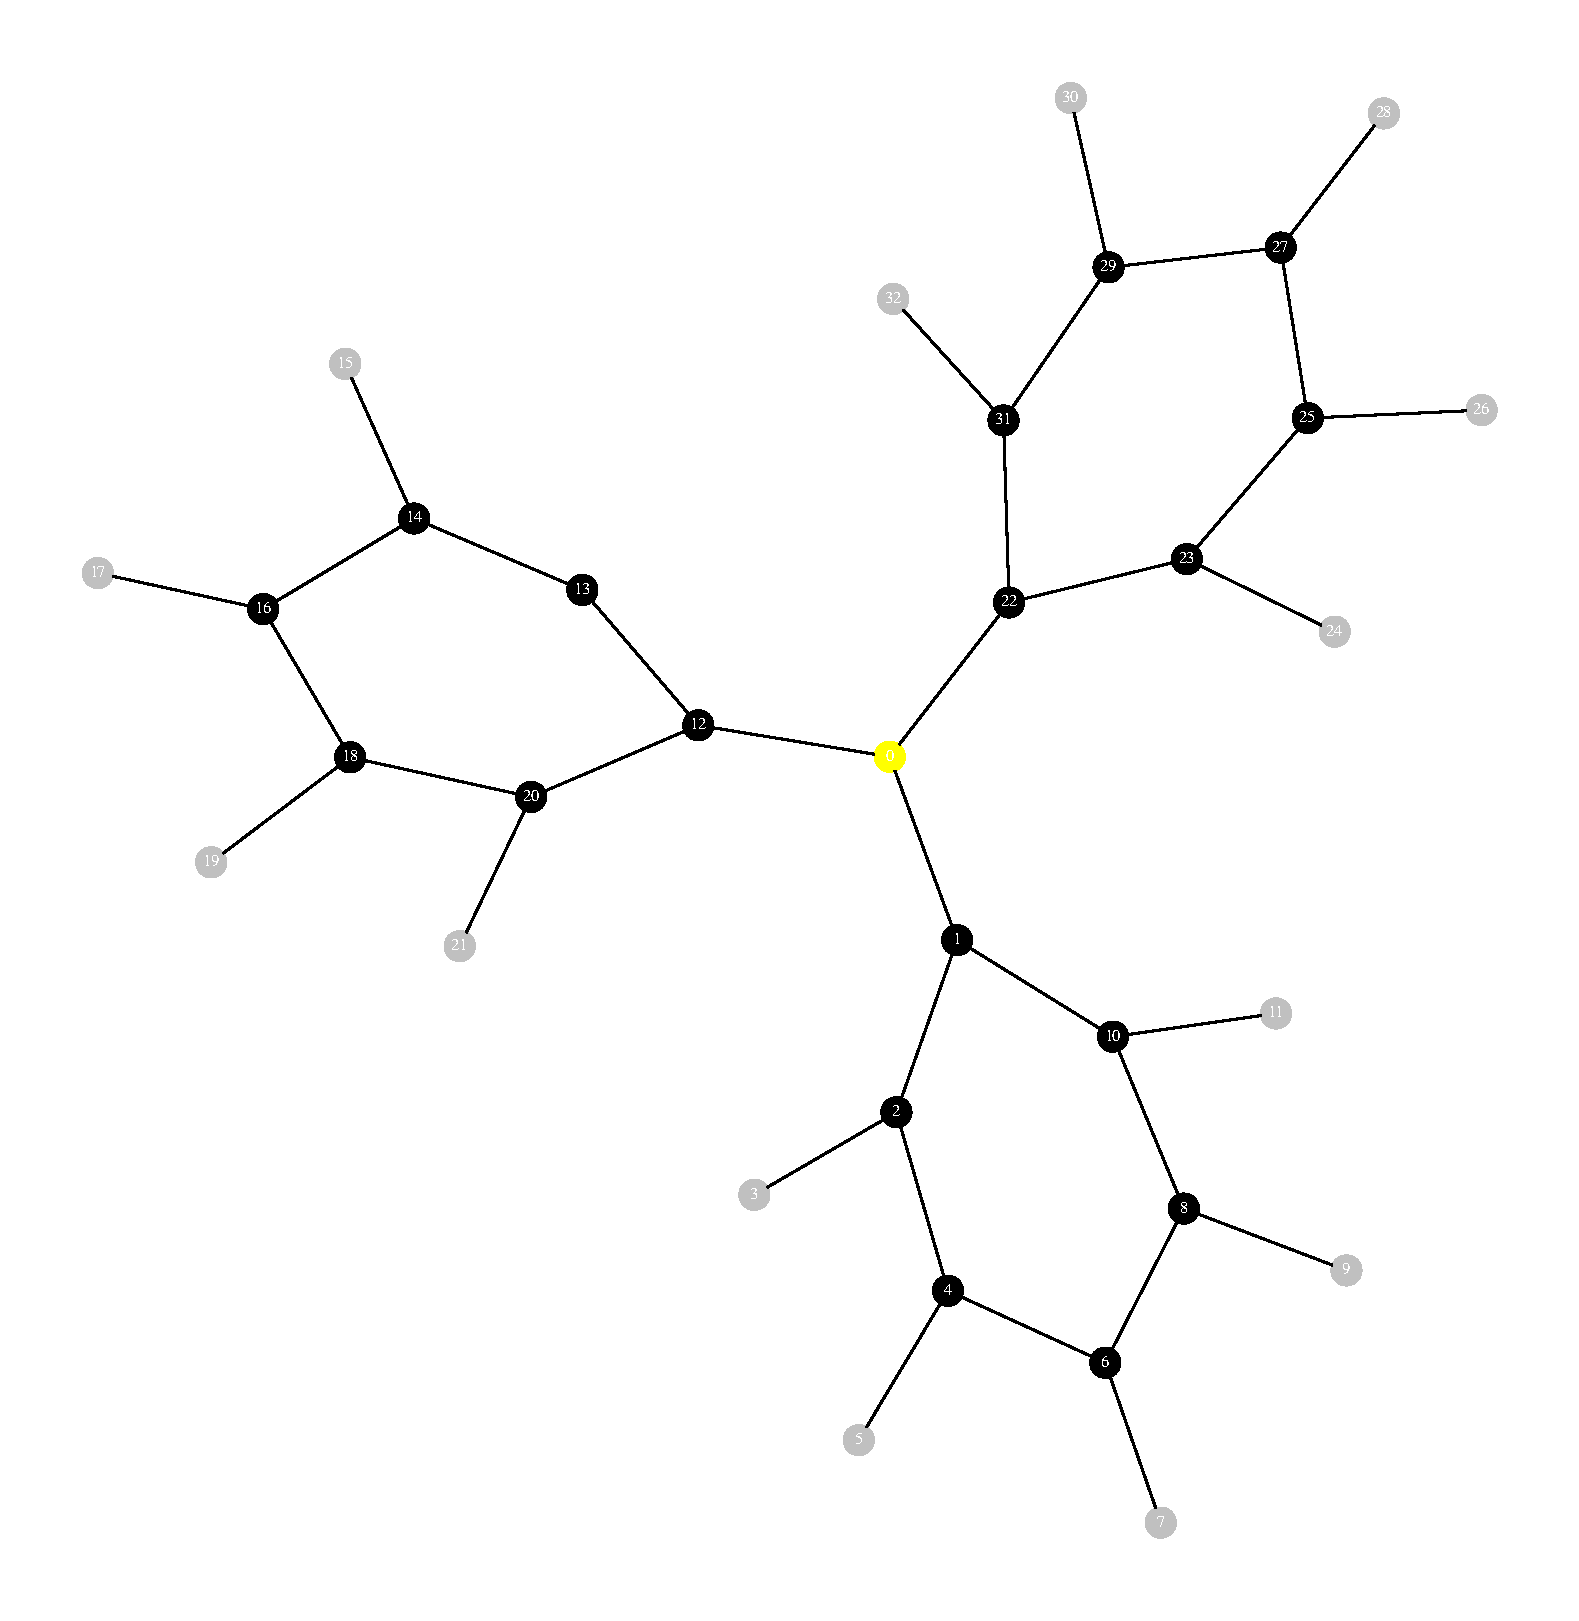
\includegraphics[scale=0.15]{mol_pictures_unfiltered/18.pdf}}

\vspace{1cm}
\begin{verbatim}
<HiPRGen.species_questions.species_default_true object at 0x2b667d6b2430>
Terminal.KEEP
\end{verbatim}


number: 19



entry id: 2aa3c4ee4b19f7b7953edb0df41b416f-C18H14S1-1-2



uncorrected free energy: -29713.82662078988



formula: C18 H14 S1

\raisebox{-.5\height}{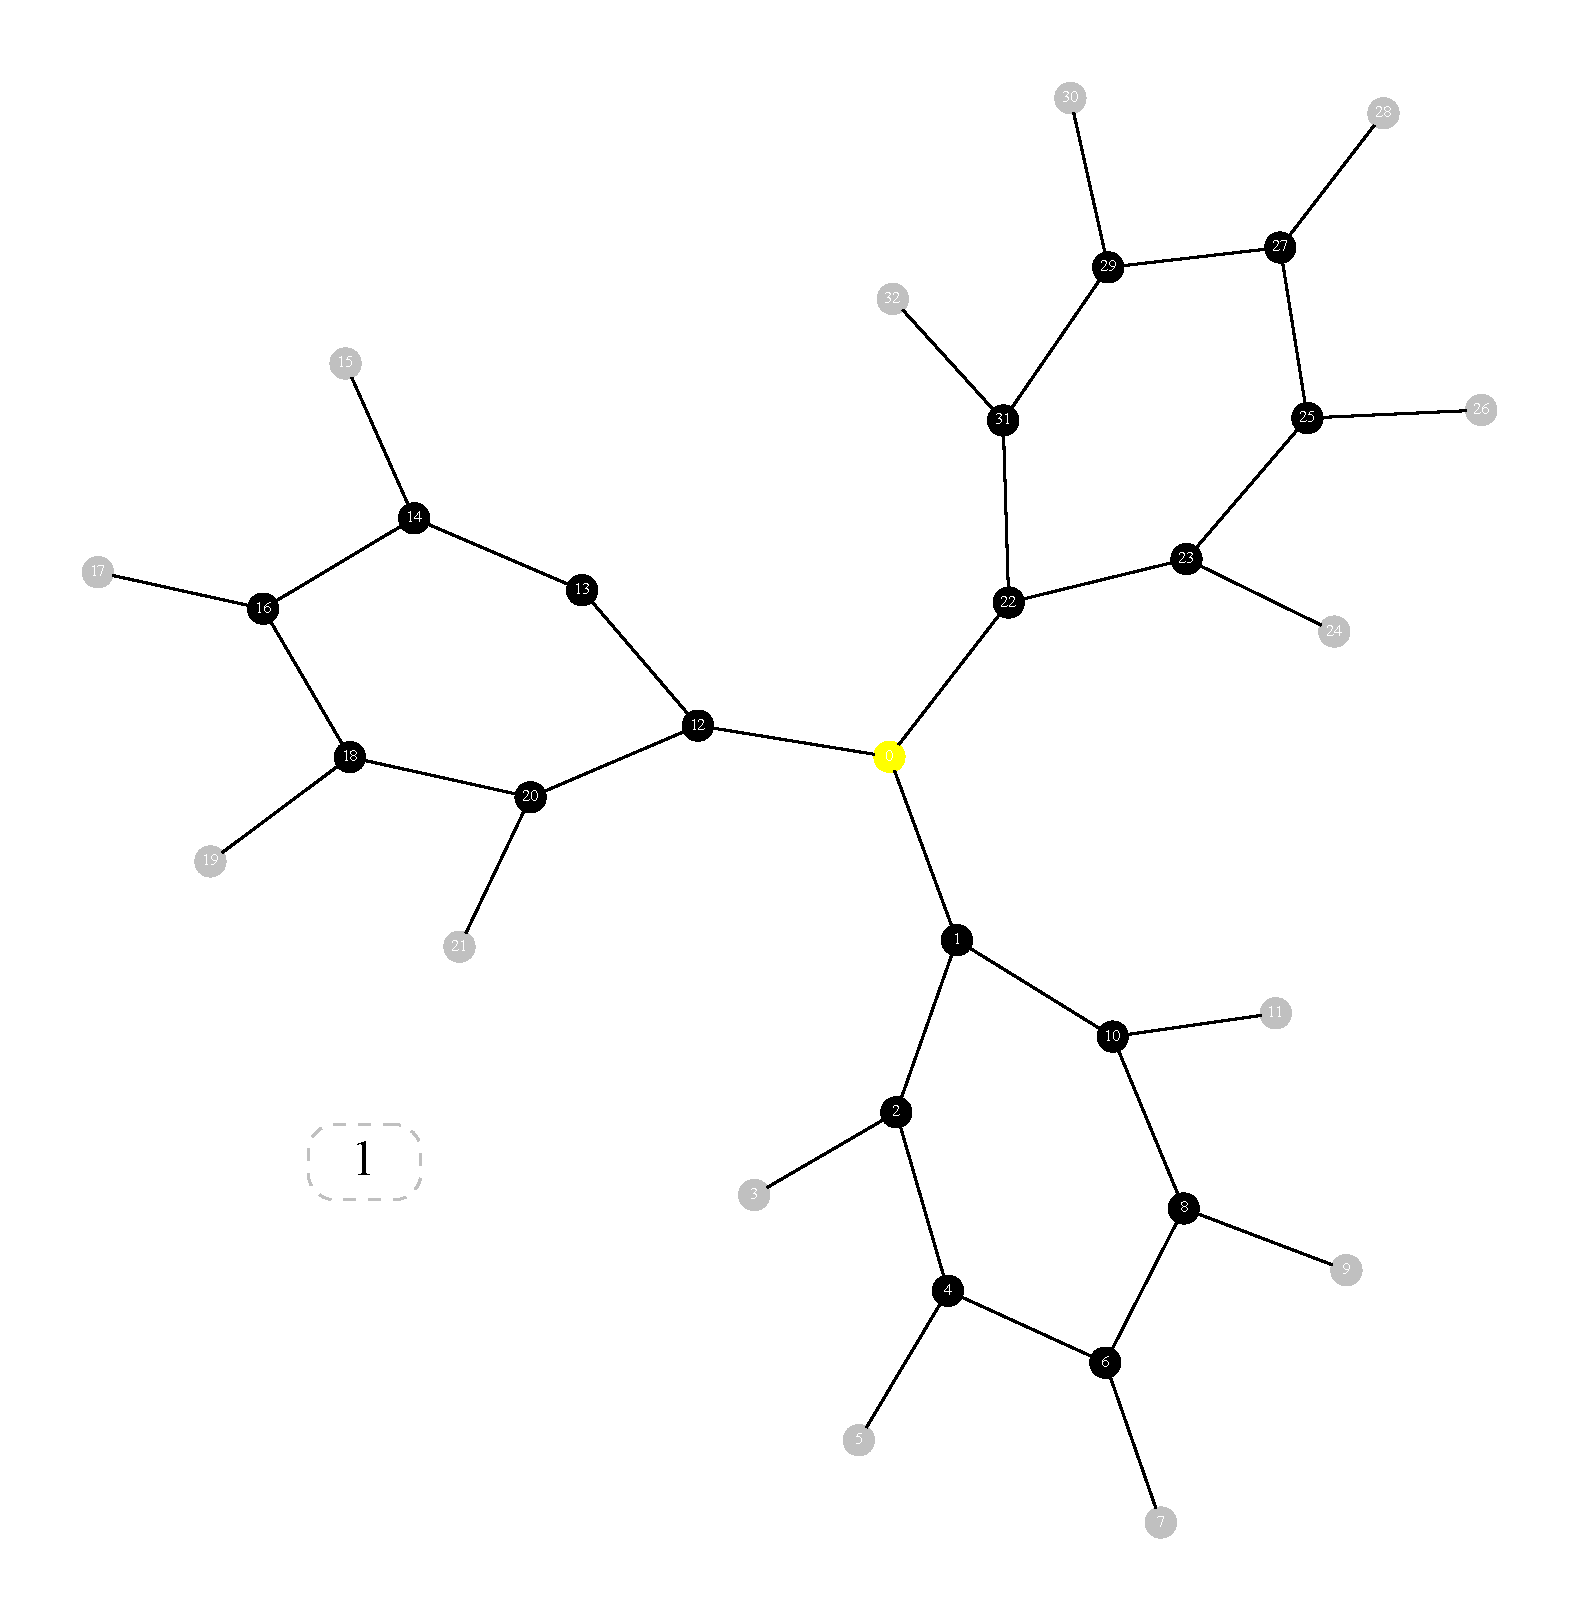
\includegraphics[scale=0.15]{mol_pictures_unfiltered/19.pdf}}

\vspace{1cm}
\begin{verbatim}
<HiPRGen.species_questions.species_default_true object at 0x2b667d6b2430>
Terminal.KEEP
\end{verbatim}


number: 20



entry id: bf707048f238a54366b2e58f3544e82f-C9H17O2-m1-1



uncorrected free energy: -13699.256050742573



formula: C9 H17 O2

\raisebox{-.5\height}{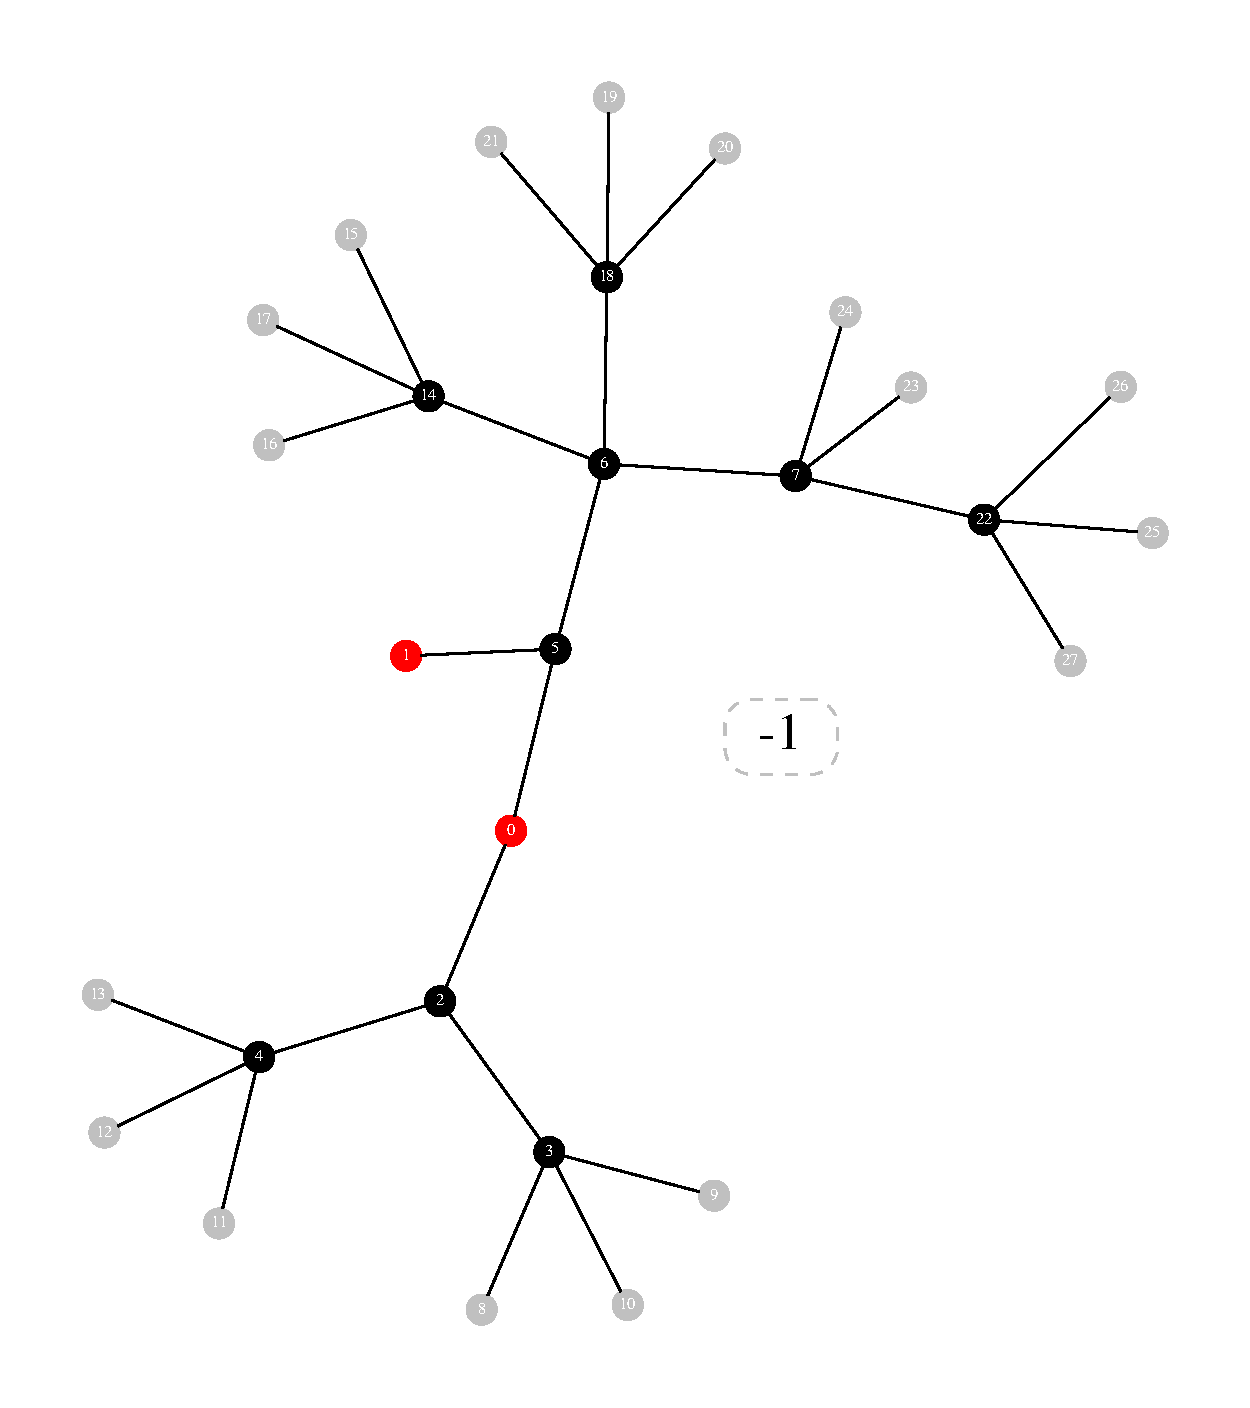
\includegraphics[scale=0.15]{mol_pictures_unfiltered/20.pdf}}

\vspace{1cm}
\begin{verbatim}
<HiPRGen.species_questions.species_default_true object at 0x2b667d6b2430>
Terminal.KEEP
\end{verbatim}


number: 21



entry id: 00dc803a2a2dd2005acbb5d51b71a7d7-C9H17O2-0-2



uncorrected free energy: -13697.297882450022



formula: C9 H17 O2

\raisebox{-.5\height}{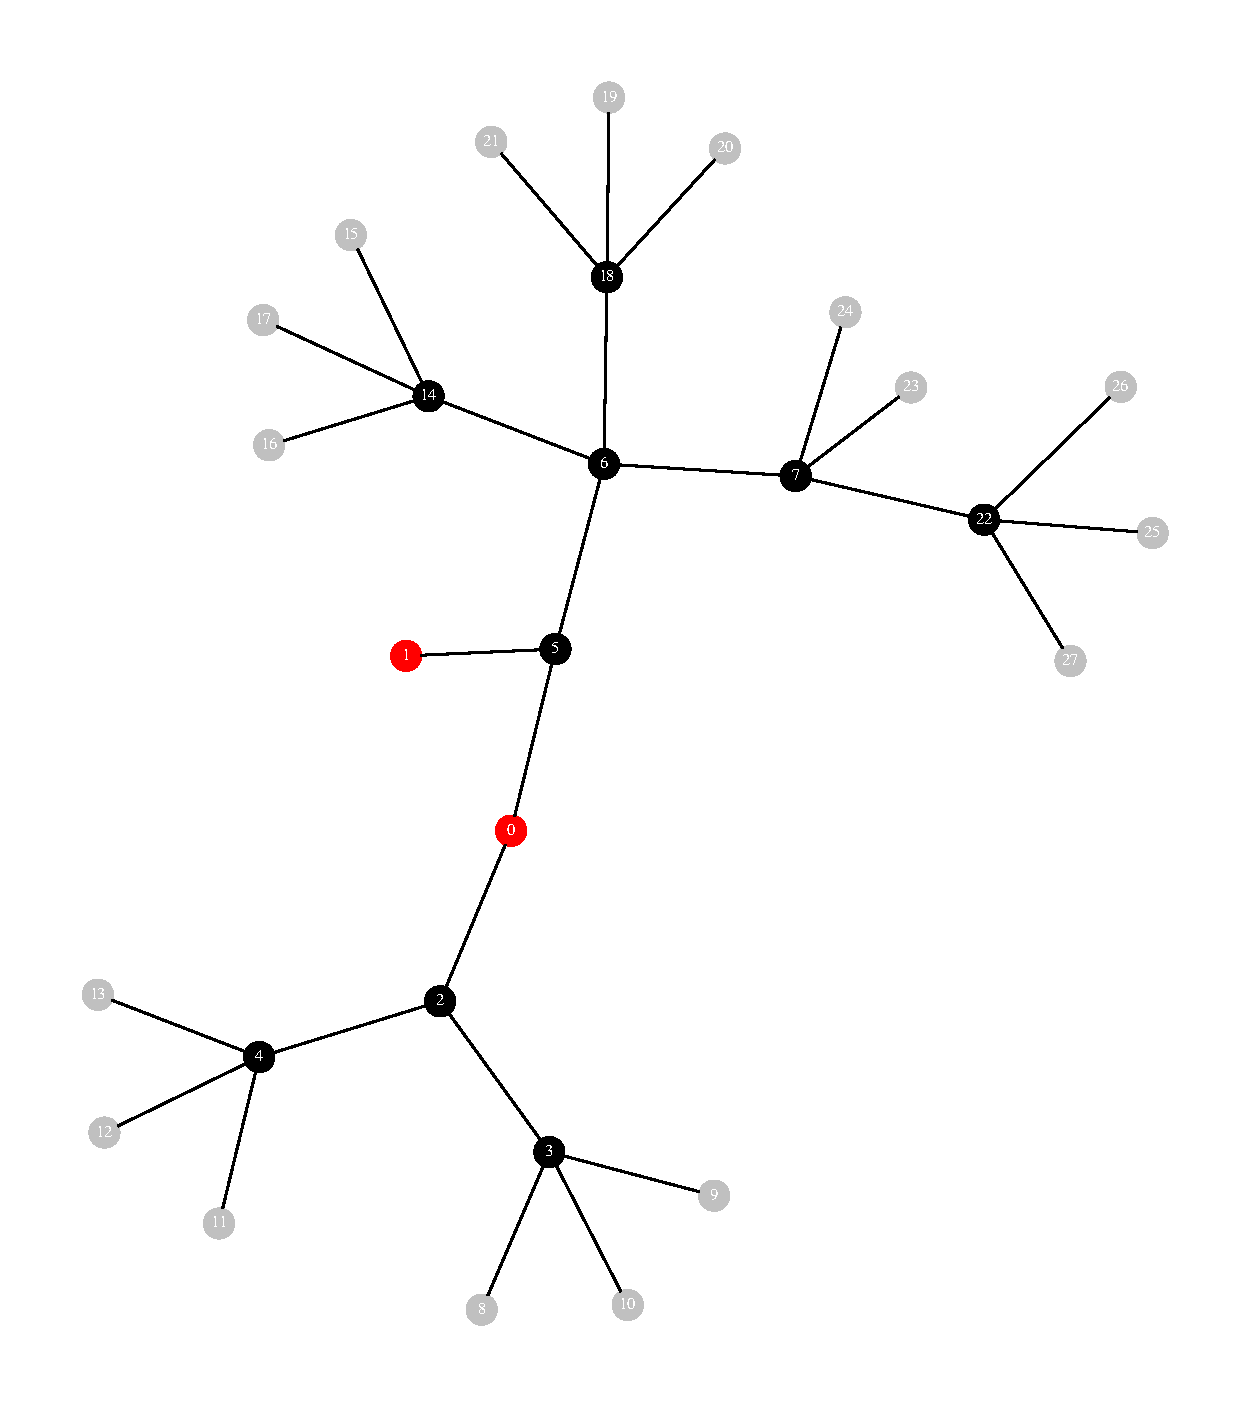
\includegraphics[scale=0.15]{mol_pictures_unfiltered/21.pdf}}

\vspace{1cm}
\begin{verbatim}
<HiPRGen.species_questions.species_default_true object at 0x2b667d6b2430>
Terminal.KEEP
\end{verbatim}


number: 22



entry id: ef9885d298317f560d763c1c9df88ea7-C9H17O2-1-1



uncorrected free energy: -13692.483353819382



formula: C9 H17 O2

\raisebox{-.5\height}{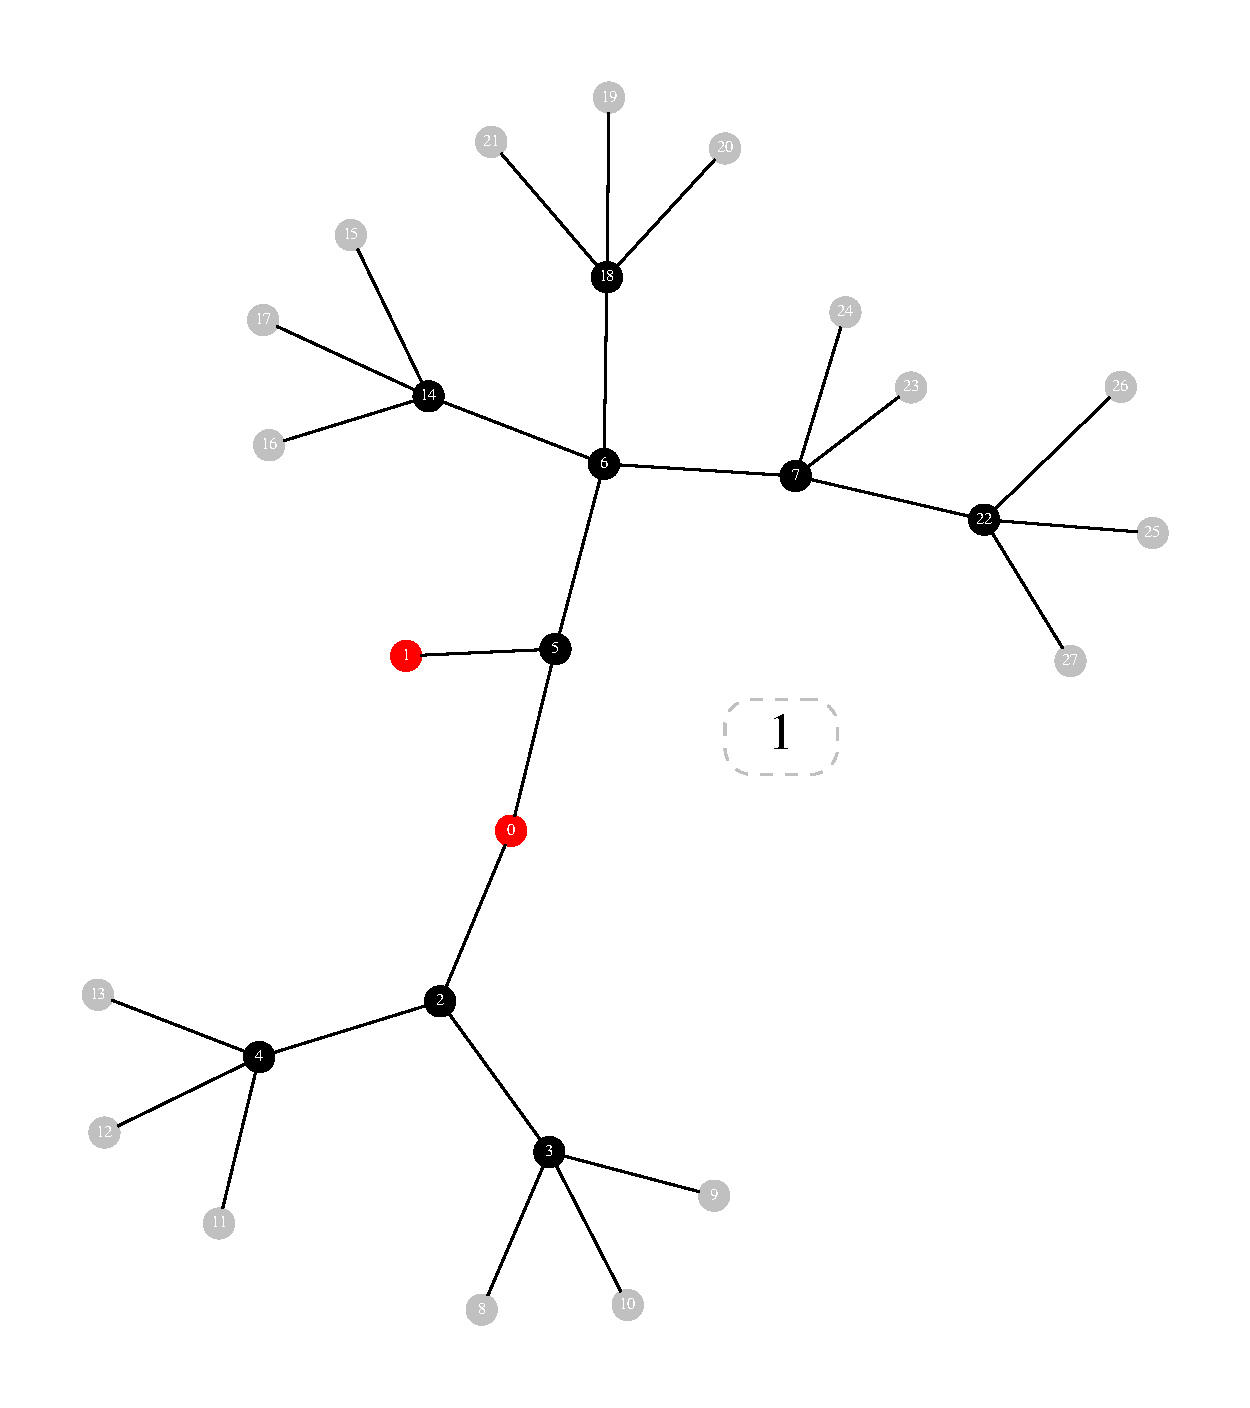
\includegraphics[scale=0.15]{mol_pictures_unfiltered/22.pdf}}

\vspace{1cm}
\begin{verbatim}
<HiPRGen.species_questions.species_default_true object at 0x2b667d6b2430>
Terminal.KEEP
\end{verbatim}


number: 23



entry id: ace47f1afdf09aea2d7a88313246cf5e-C16H19S1-0-2



uncorrected free energy: -27725.461978143005



formula: C16 H19 S1

\raisebox{-.5\height}{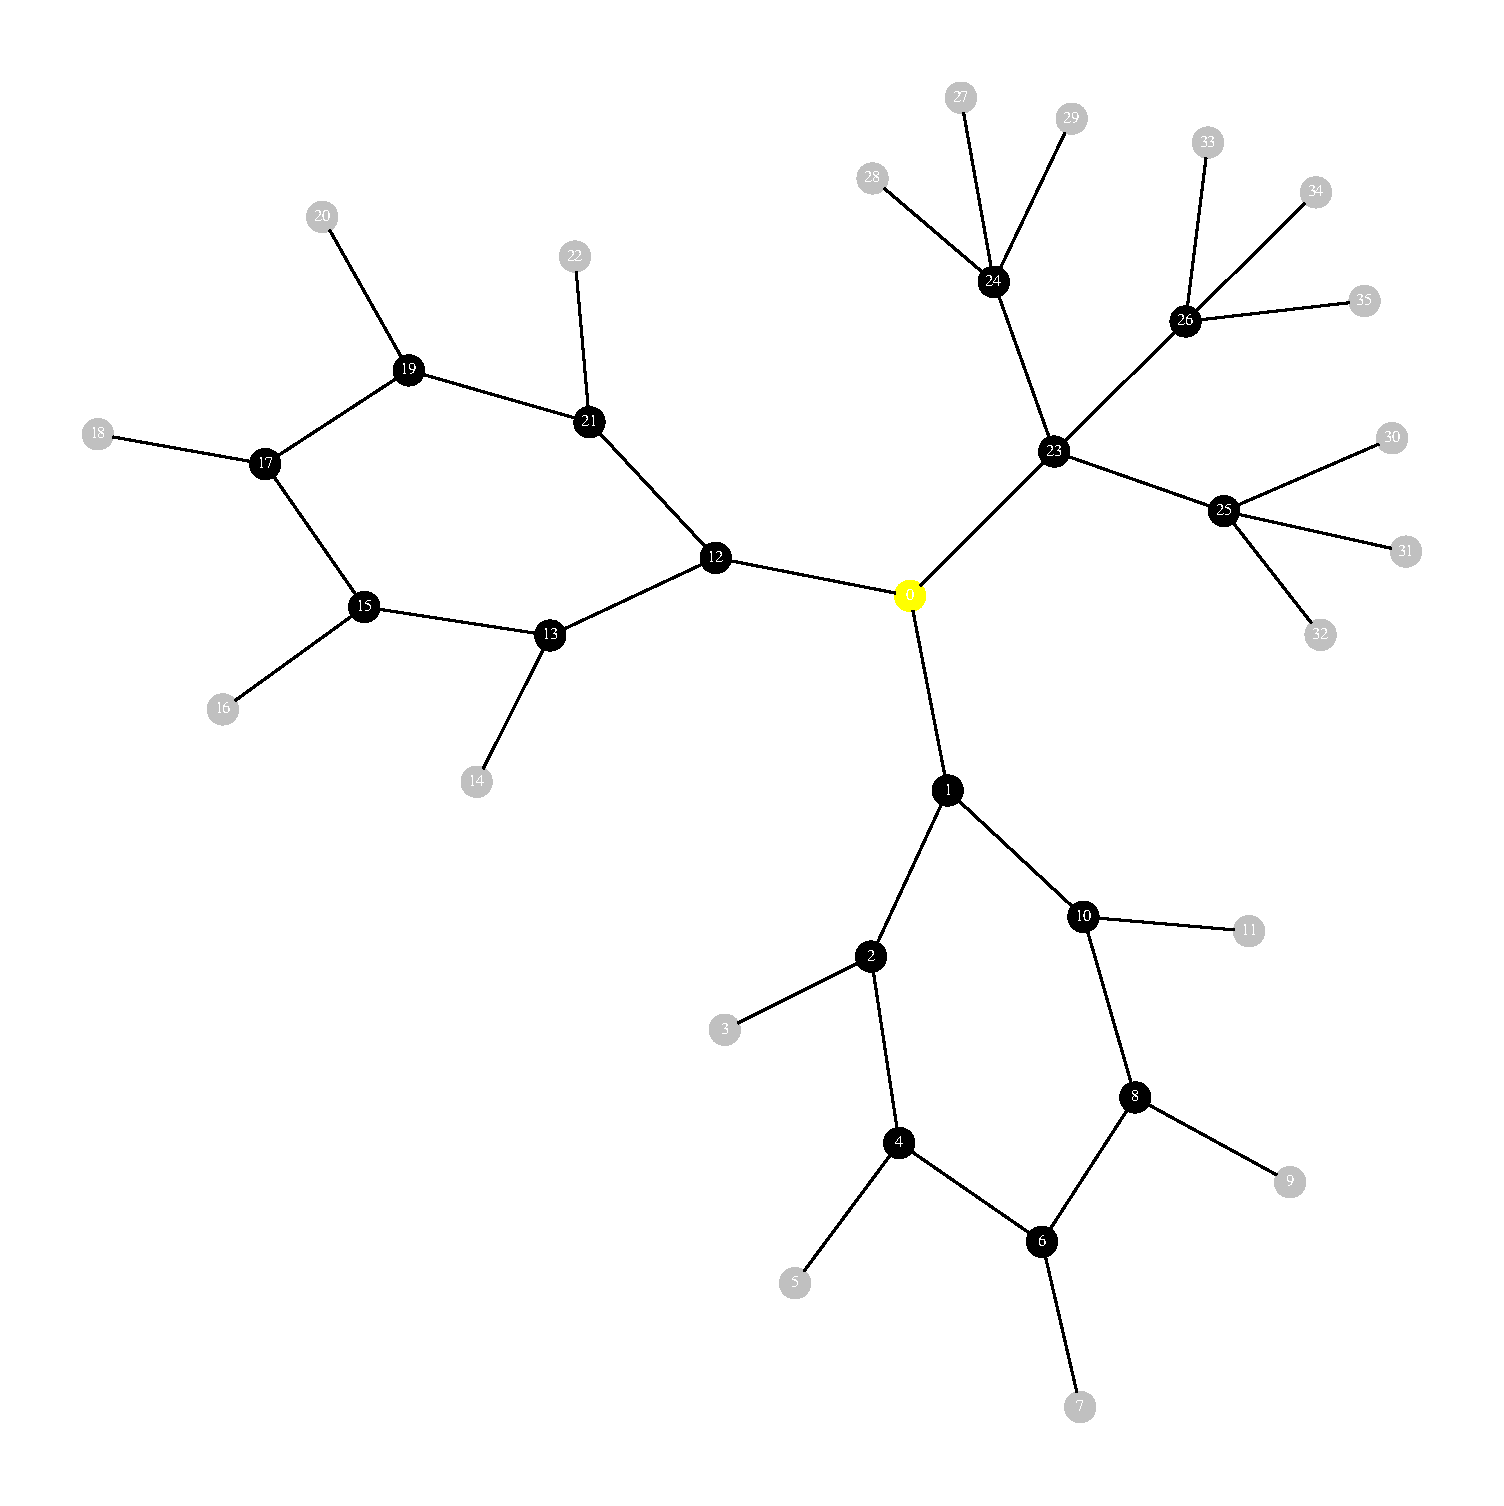
\includegraphics[scale=0.15]{mol_pictures_unfiltered/23.pdf}}

\vspace{1cm}
\begin{verbatim}
<HiPRGen.species_questions.species_default_true object at 0x2b667d6b2430>
Terminal.KEEP
\end{verbatim}


number: 24



entry id: b753e8d3829ebe4c1b93bf339690d319-C16H19S1-1-1



uncorrected free energy: -27722.57399714871



formula: C16 H19 S1

\raisebox{-.5\height}{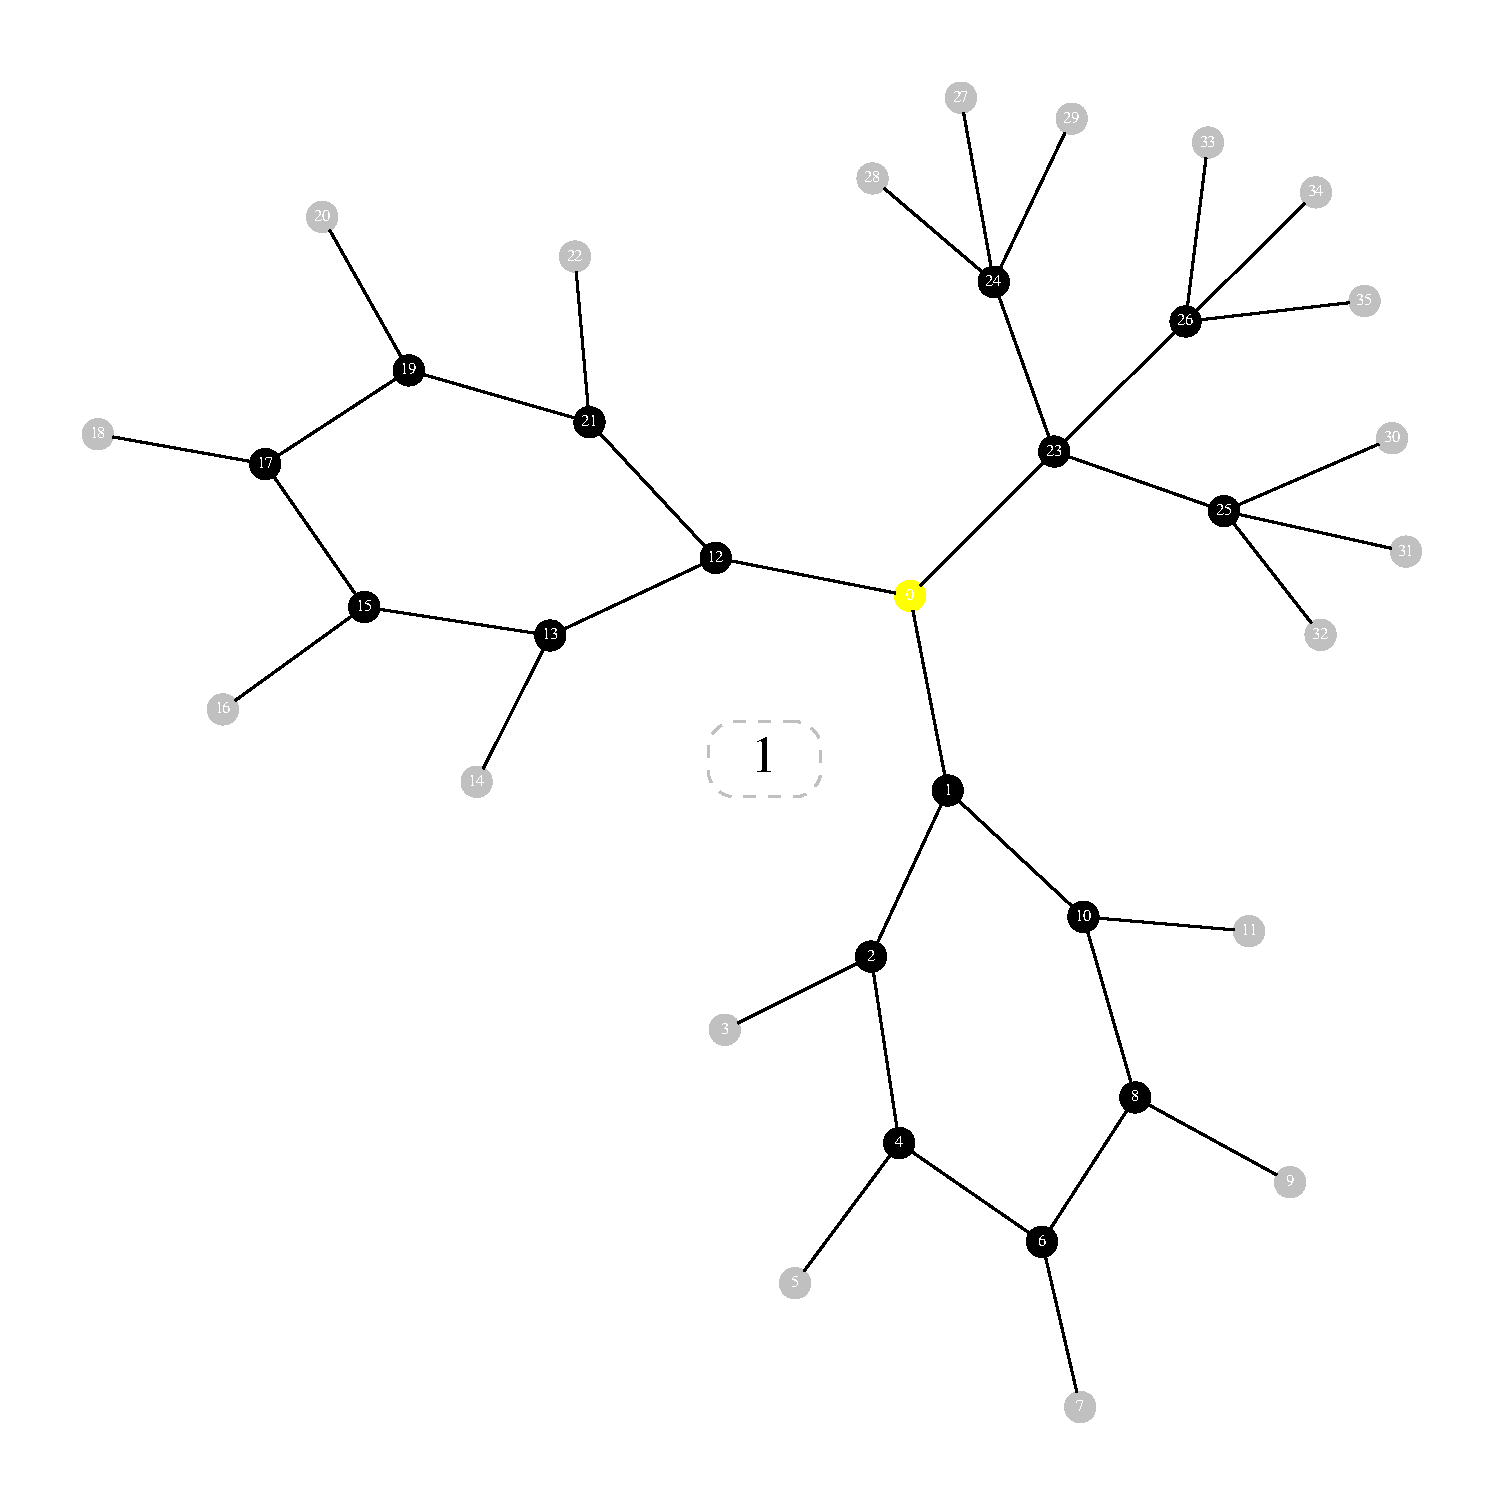
\includegraphics[scale=0.15]{mol_pictures_unfiltered/24.pdf}}

\vspace{1cm}
\begin{verbatim}
<HiPRGen.species_questions.species_default_true object at 0x2b667d6b2430>
Terminal.KEEP
\end{verbatim}


number: 25



entry id: f70a294e2348dc611a45088494876955-C4H10-m1-2



uncorrected free energy: -4306.996405540511



formula: C4 H10

\raisebox{-.5\height}{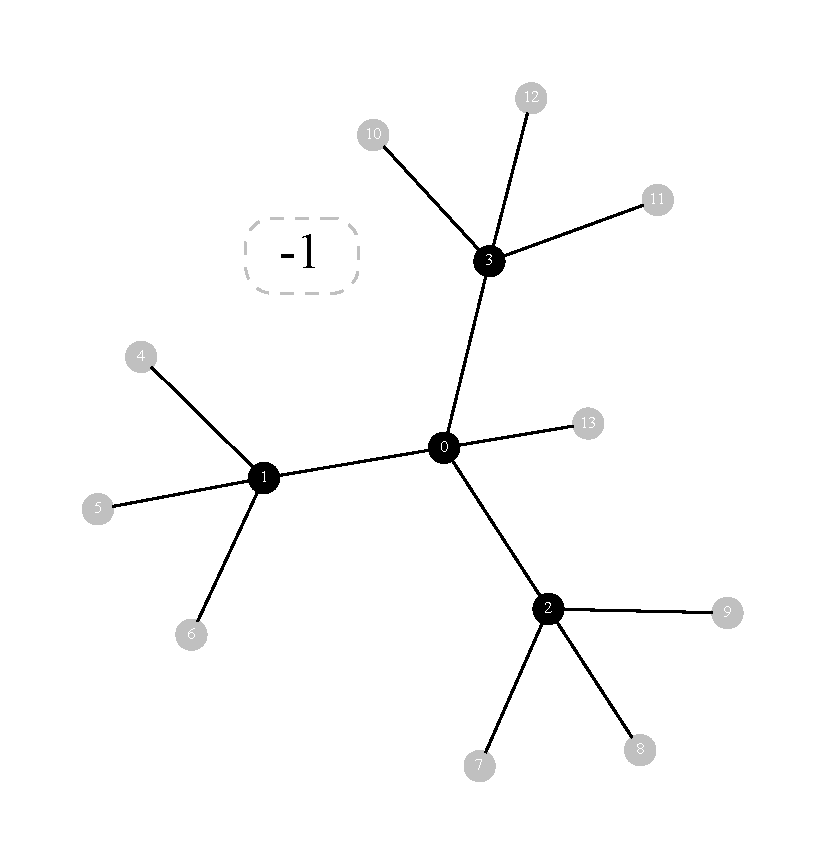
\includegraphics[scale=0.15]{mol_pictures_unfiltered/25.pdf}}

\vspace{1cm}
\begin{verbatim}
<HiPRGen.species_questions.species_default_true object at 0x2b667d6b2430>
Terminal.KEEP
\end{verbatim}


number: 26



entry id: eea050c031d211549457abfc44b469a9-C4H10-0-1



uncorrected free energy: -4307.494049512899



formula: C4 H10

\raisebox{-.5\height}{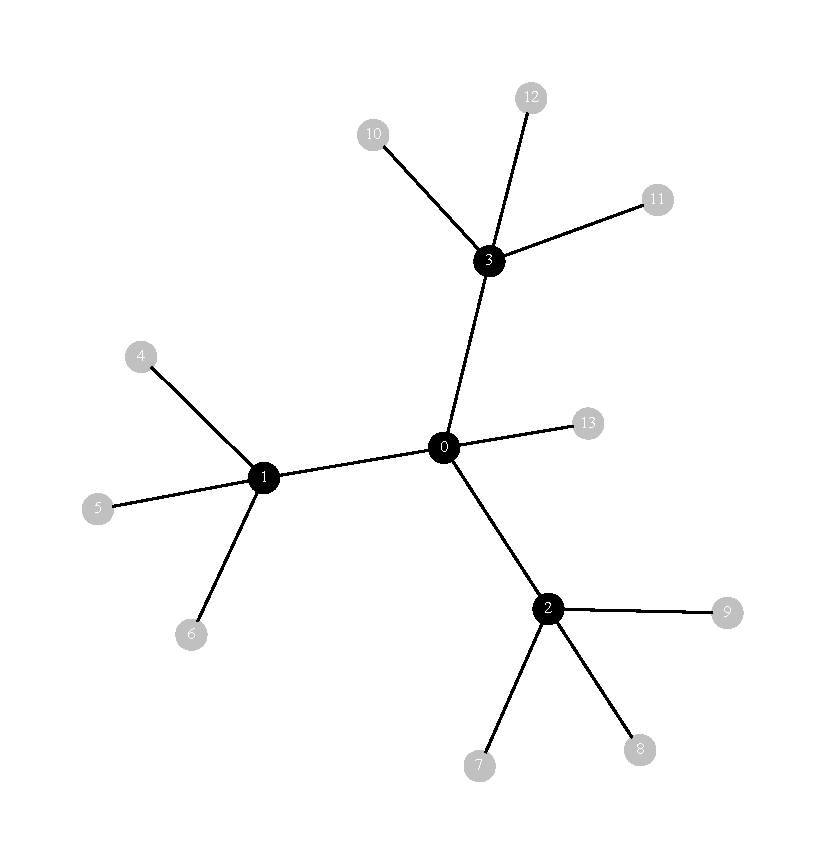
\includegraphics[scale=0.15]{mol_pictures_unfiltered/26.pdf}}

\vspace{1cm}
\begin{verbatim}
<HiPRGen.species_questions.species_default_true object at 0x2b667d6b2430>
Terminal.KEEP
\end{verbatim}


number: 27



entry id: bff66d78cfd6b31ffe8f16b27ae69618-C4H10-1-2



uncorrected free energy: -4298.846498430801



formula: C4 H10

\raisebox{-.5\height}{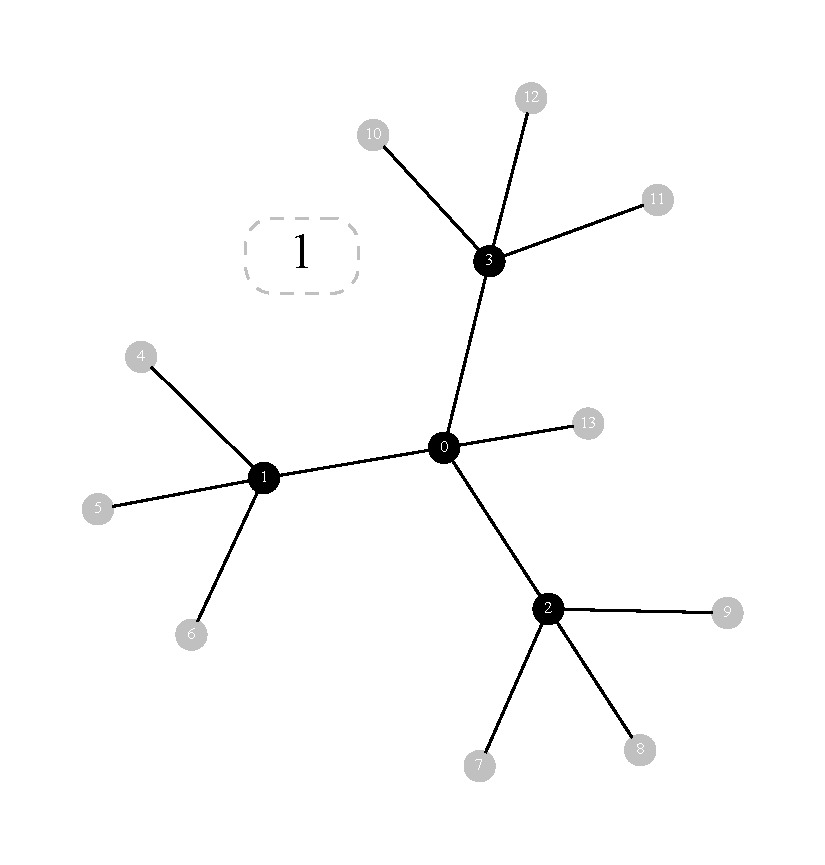
\includegraphics[scale=0.15]{mol_pictures_unfiltered/27.pdf}}

\vspace{1cm}
\begin{verbatim}
<HiPRGen.species_questions.species_default_true object at 0x2b667d6b2430>
Terminal.KEEP
\end{verbatim}


number: 28



entry id: 035975cc24e93e53983b067459690b02-C18H15S1-0-2



uncorrected free energy: -29735.095680830127



formula: C18 H15 S1

\raisebox{-.5\height}{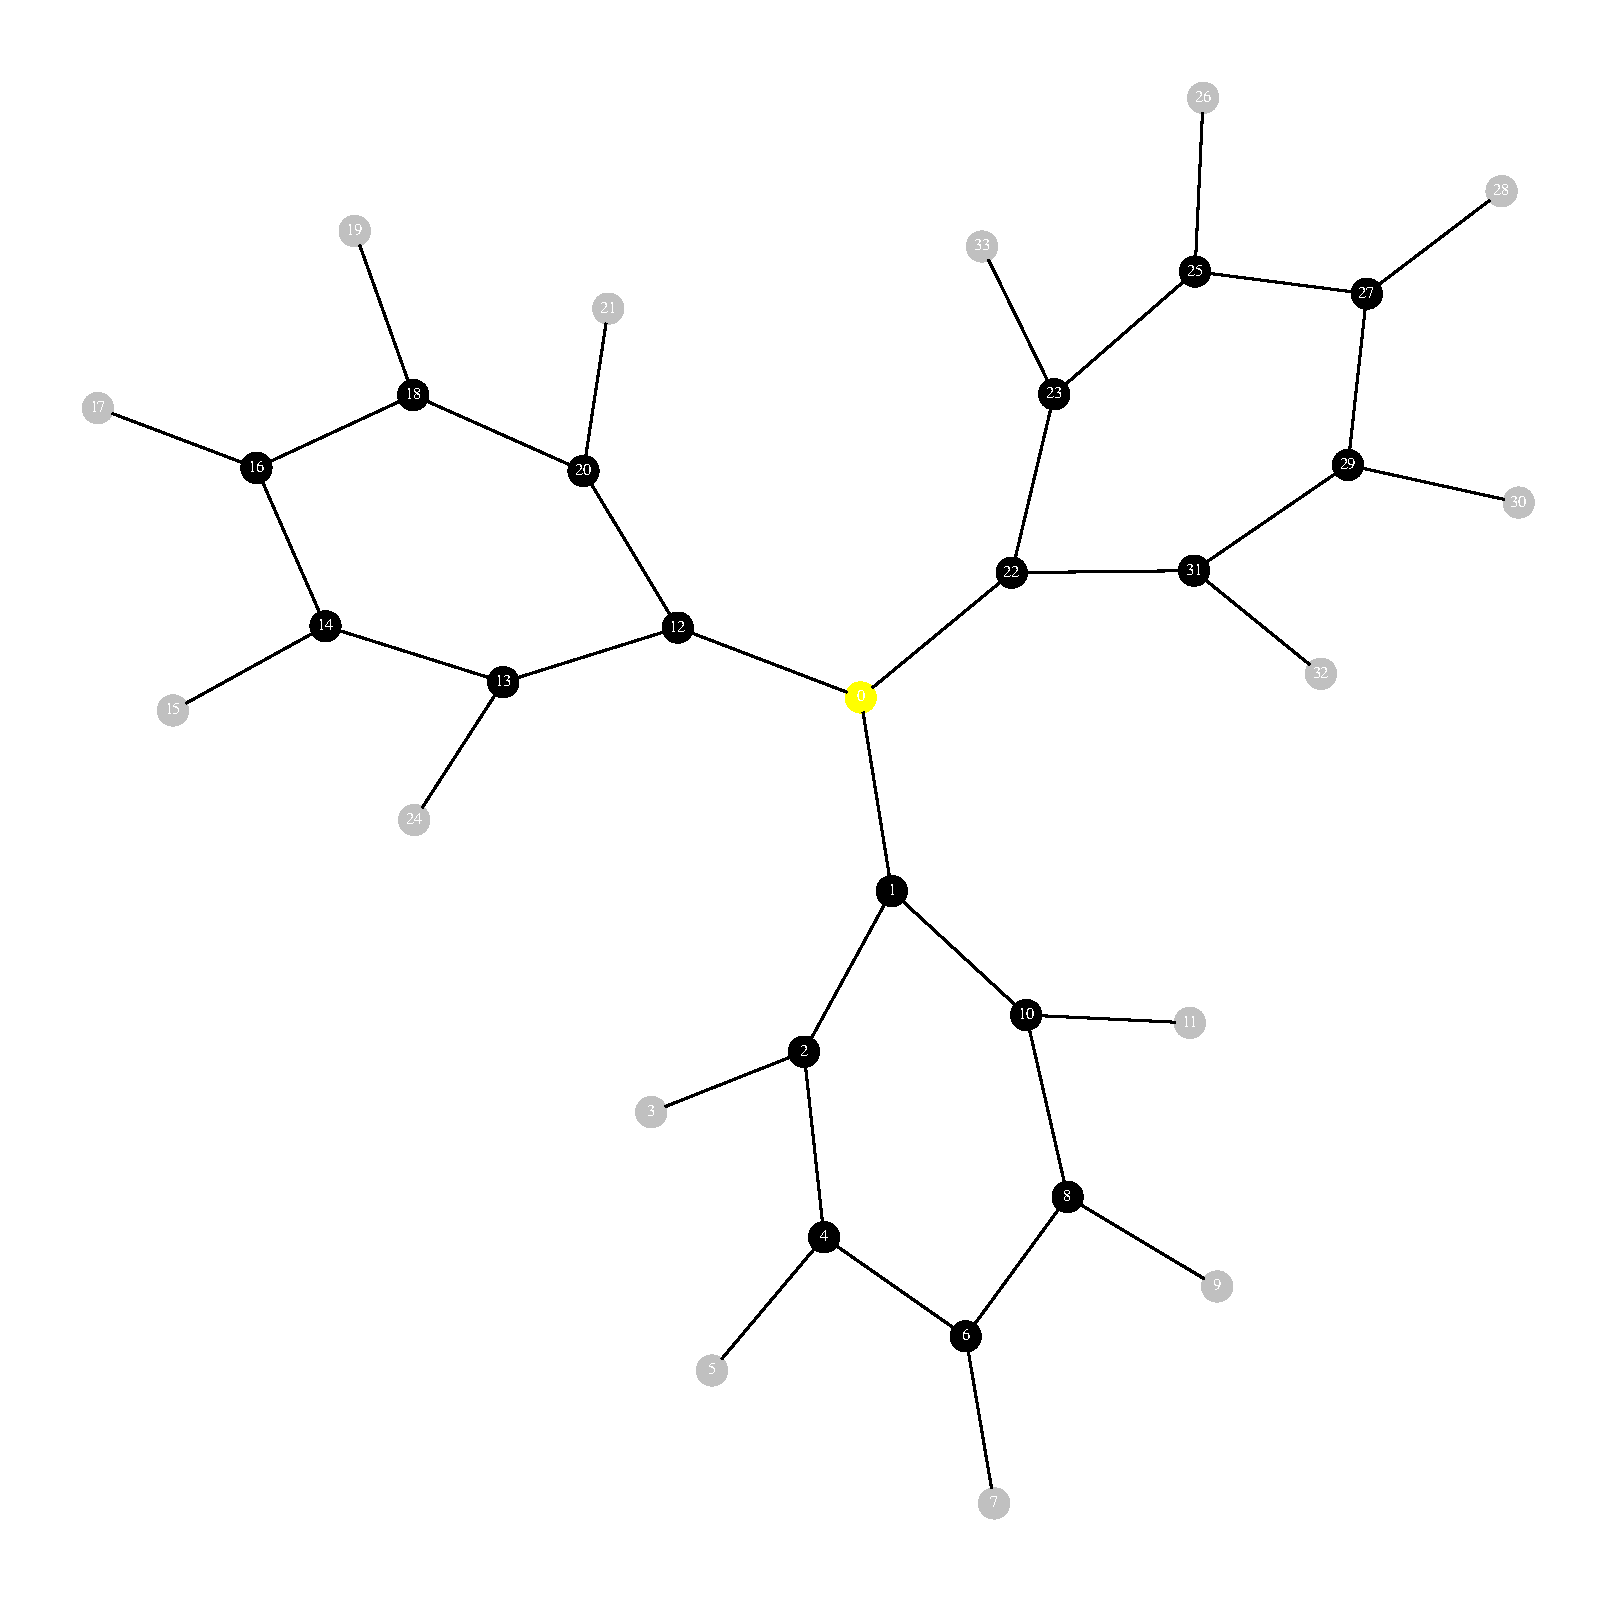
\includegraphics[scale=0.15]{mol_pictures_unfiltered/28.pdf}}

\vspace{1cm}
\begin{verbatim}
<HiPRGen.species_questions.species_default_true object at 0x2b667d6b2430>
Terminal.KEEP
\end{verbatim}


number: 29



entry id: 94be97269b03e361ba1b344f48f19e44-C18H15S1-1-1



uncorrected free energy: -29732.16832442951



formula: C18 H15 S1

\raisebox{-.5\height}{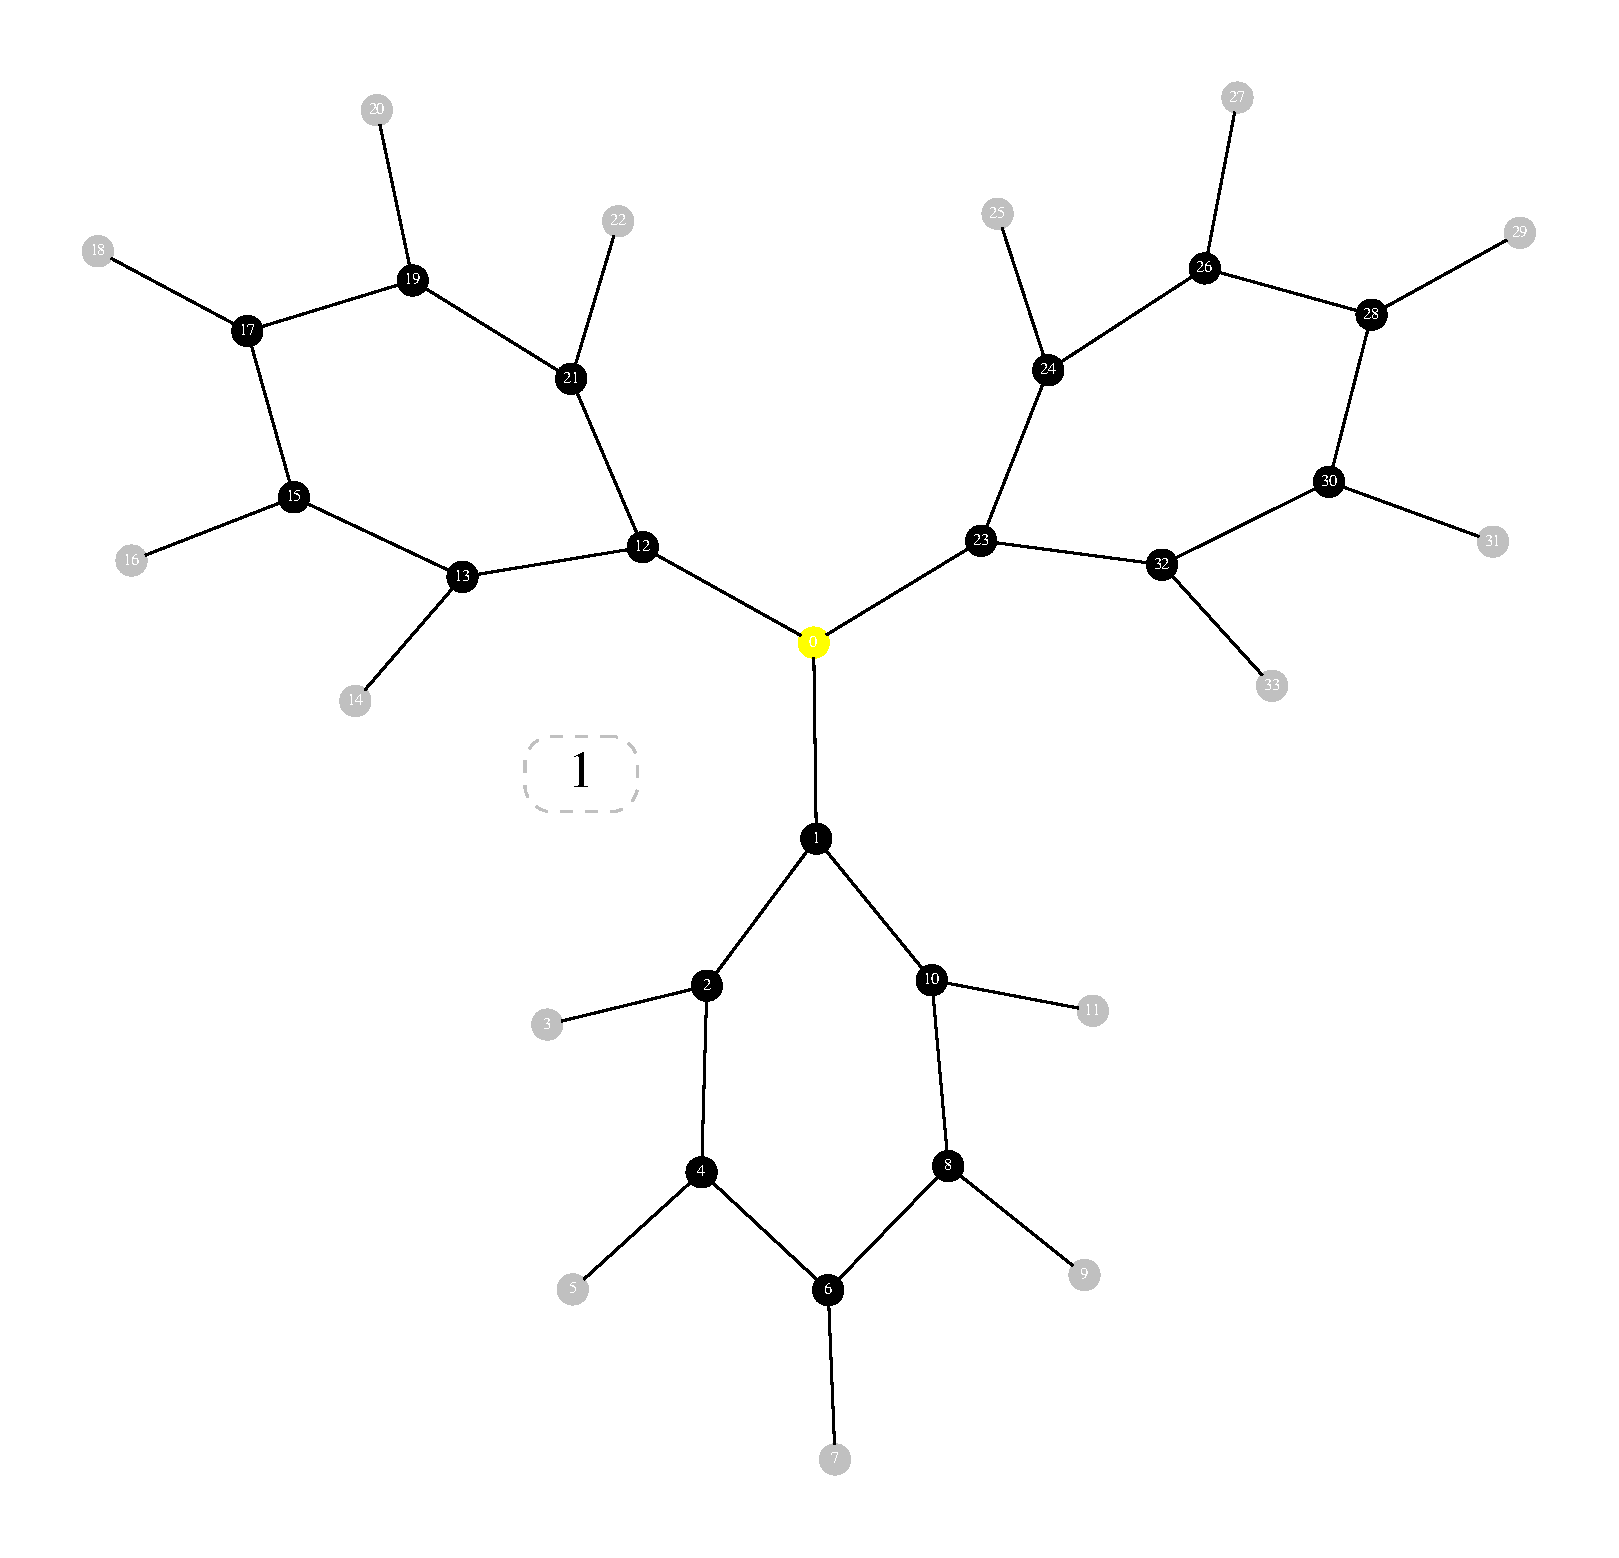
\includegraphics[scale=0.15]{mol_pictures_unfiltered/29.pdf}}

\vspace{1cm}
\begin{verbatim}
<HiPRGen.species_questions.species_default_true object at 0x2b667d6b2430>
Terminal.KEEP
\end{verbatim}


number: 30



entry id: 03fa2887bf9301307bdf24d123f68795-C18H15S1-2-2



uncorrected free energy: -29722.855017808004



formula: C18 H15 S1

\raisebox{-.5\height}{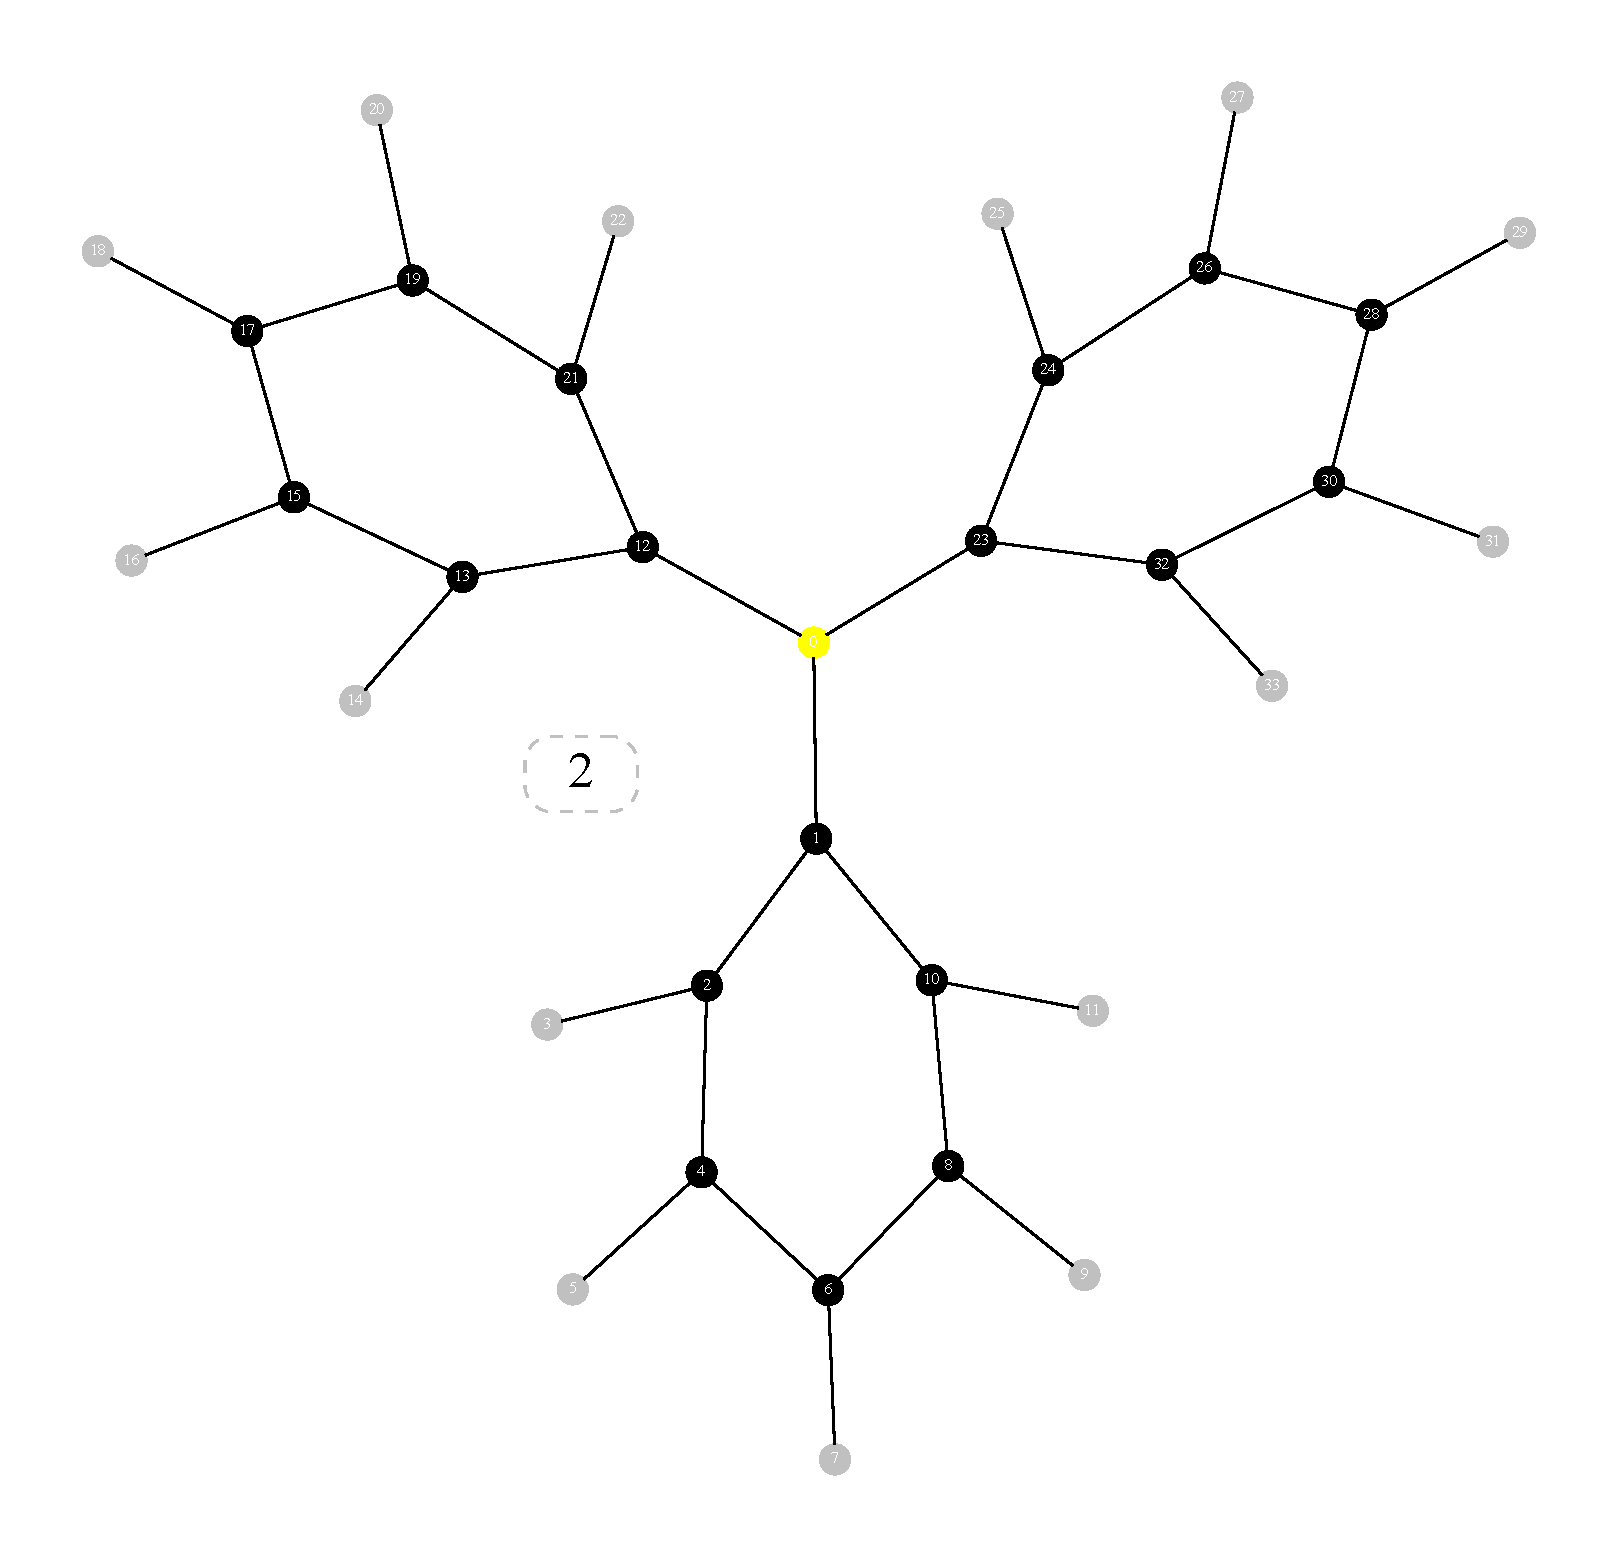
\includegraphics[scale=0.15]{mol_pictures_unfiltered/30.pdf}}

\vspace{1cm}
\begin{verbatim}
<HiPRGen.species_questions.species_default_true object at 0x2b667d6b2430>
Terminal.KEEP
\end{verbatim}


number: 31



entry id: 6abc9e860814179fef28aabbe09d1571-C1O2-0-1



uncorrected free energy: -5133.019132421511



formula: C1 O2

\raisebox{-.5\height}{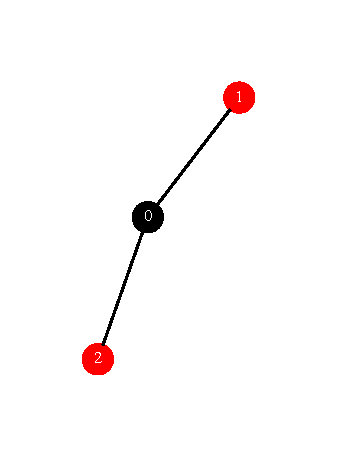
\includegraphics[scale=0.15]{mol_pictures_unfiltered/31.pdf}}

\vspace{1cm}
\begin{verbatim}
<HiPRGen.species_questions.species_default_true object at 0x2b667d6b2430>
Terminal.KEEP
\end{verbatim}


number: 32



entry id: 63a94c85aea3114c3e2baa7a790f2dcc-C4H9-m1-1



uncorrected free energy: -4291.406620223405



formula: C4 H9

\raisebox{-.5\height}{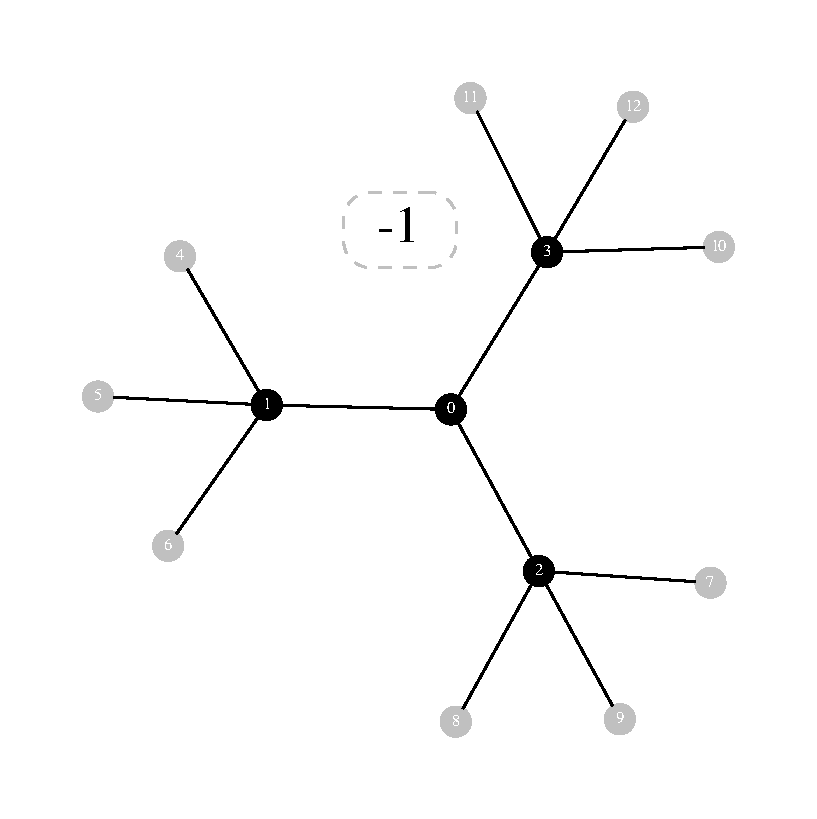
\includegraphics[scale=0.15]{mol_pictures_unfiltered/32.pdf}}

\vspace{1cm}
\begin{verbatim}
<HiPRGen.species_questions.species_default_true object at 0x2b667d6b2430>
Terminal.KEEP
\end{verbatim}


number: 33



entry id: 53e9047861139aaf2a4fff70dc49d701-C4H9-0-2



uncorrected free energy: -4290.035016715747



formula: C4 H9

\raisebox{-.5\height}{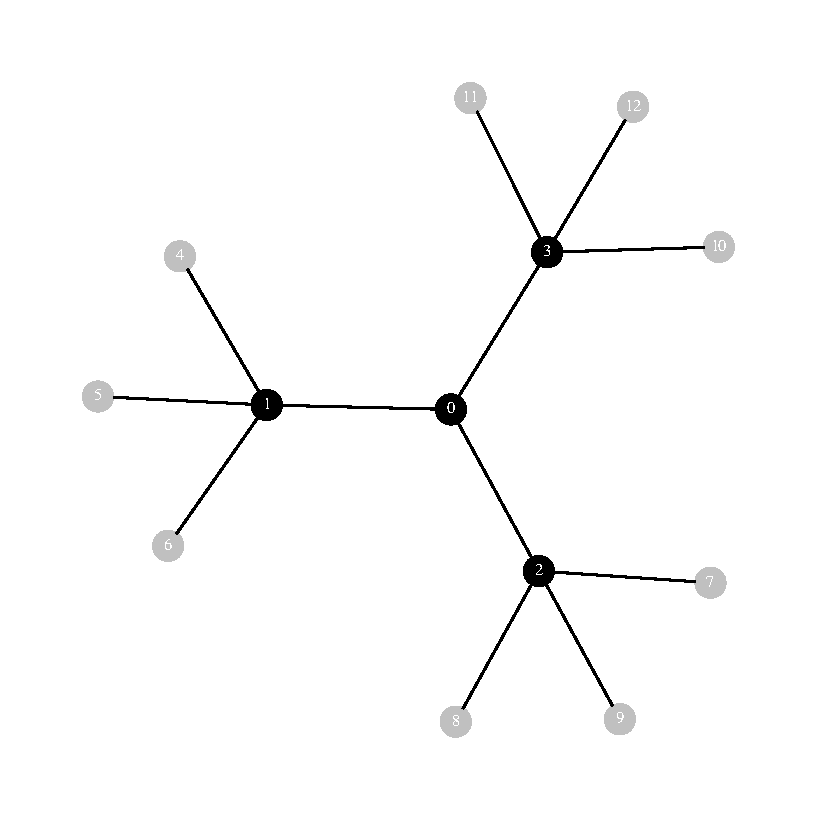
\includegraphics[scale=0.15]{mol_pictures_unfiltered/33.pdf}}

\vspace{1cm}
\begin{verbatim}
<HiPRGen.species_questions.species_default_true object at 0x2b667d6b2430>
Terminal.KEEP
\end{verbatim}


number: 34



entry id: 2f4051ef4b3969cbf0d7a51a3d57959e-C4H9-1-1



uncorrected free energy: -4284.999866720066



formula: C4 H9

\raisebox{-.5\height}{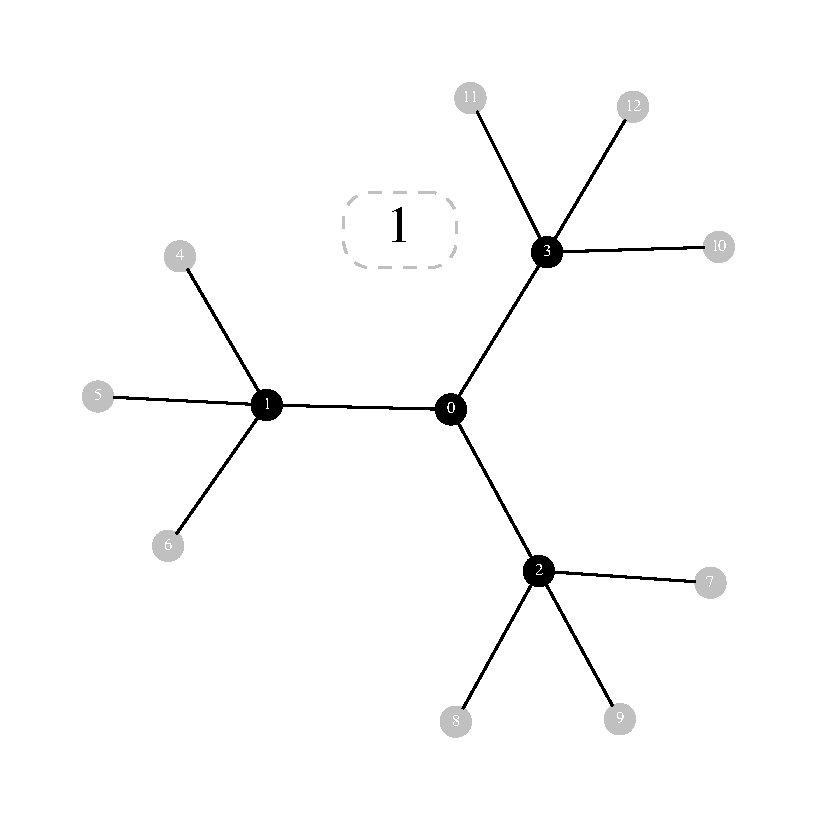
\includegraphics[scale=0.15]{mol_pictures_unfiltered/34.pdf}}

\vspace{1cm}
\begin{verbatim}
<HiPRGen.species_questions.species_default_true object at 0x2b667d6b2430>
Terminal.KEEP
\end{verbatim}


number: 35



entry id: c765bf785ca367e07df60e89c5fe5e8d-C23H26S1-m1-2



uncorrected free energy: -35096.309034517726



formula: C23 H26 S1

\raisebox{-.5\height}{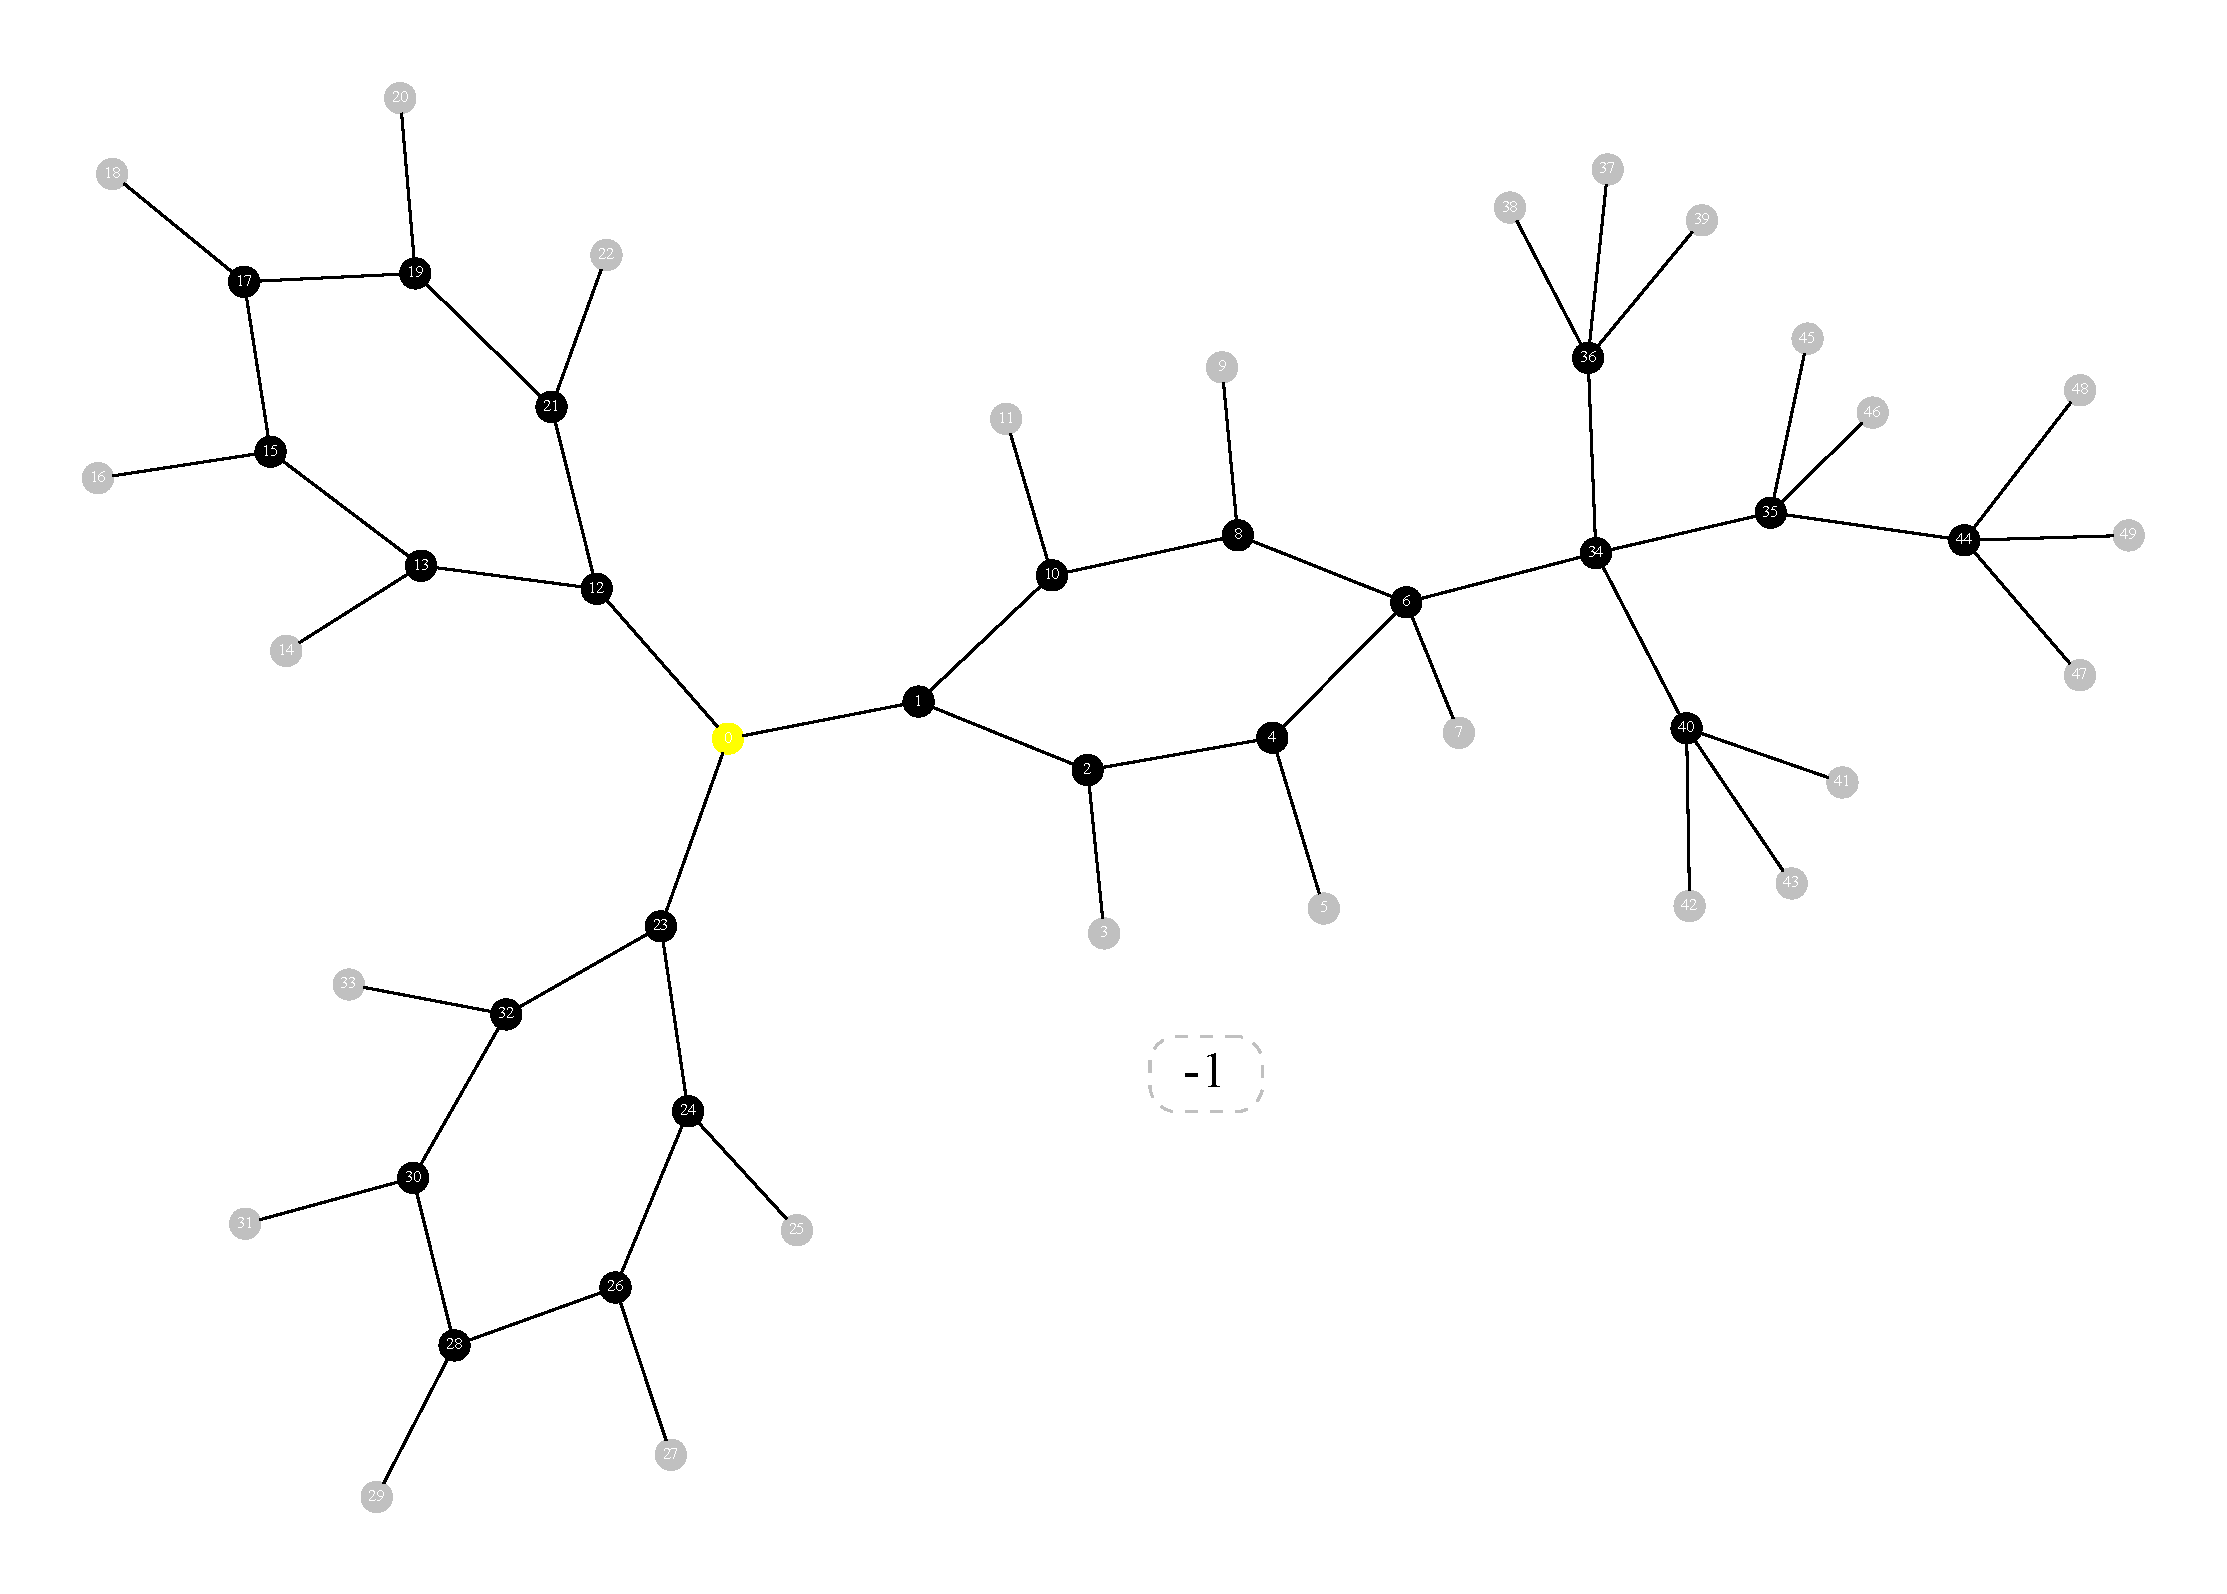
\includegraphics[scale=0.15]{mol_pictures_unfiltered/35.pdf}}

\vspace{1cm}
\begin{verbatim}
<HiPRGen.species_questions.species_default_true object at 0x2b667d6b2430>
Terminal.KEEP
\end{verbatim}


number: 36



entry id: 93d061fd43eaf14c5fc8c73be52da15b-C23H26S1-0-1



uncorrected free energy: -35095.28371038775



formula: C23 H26 S1

\raisebox{-.5\height}{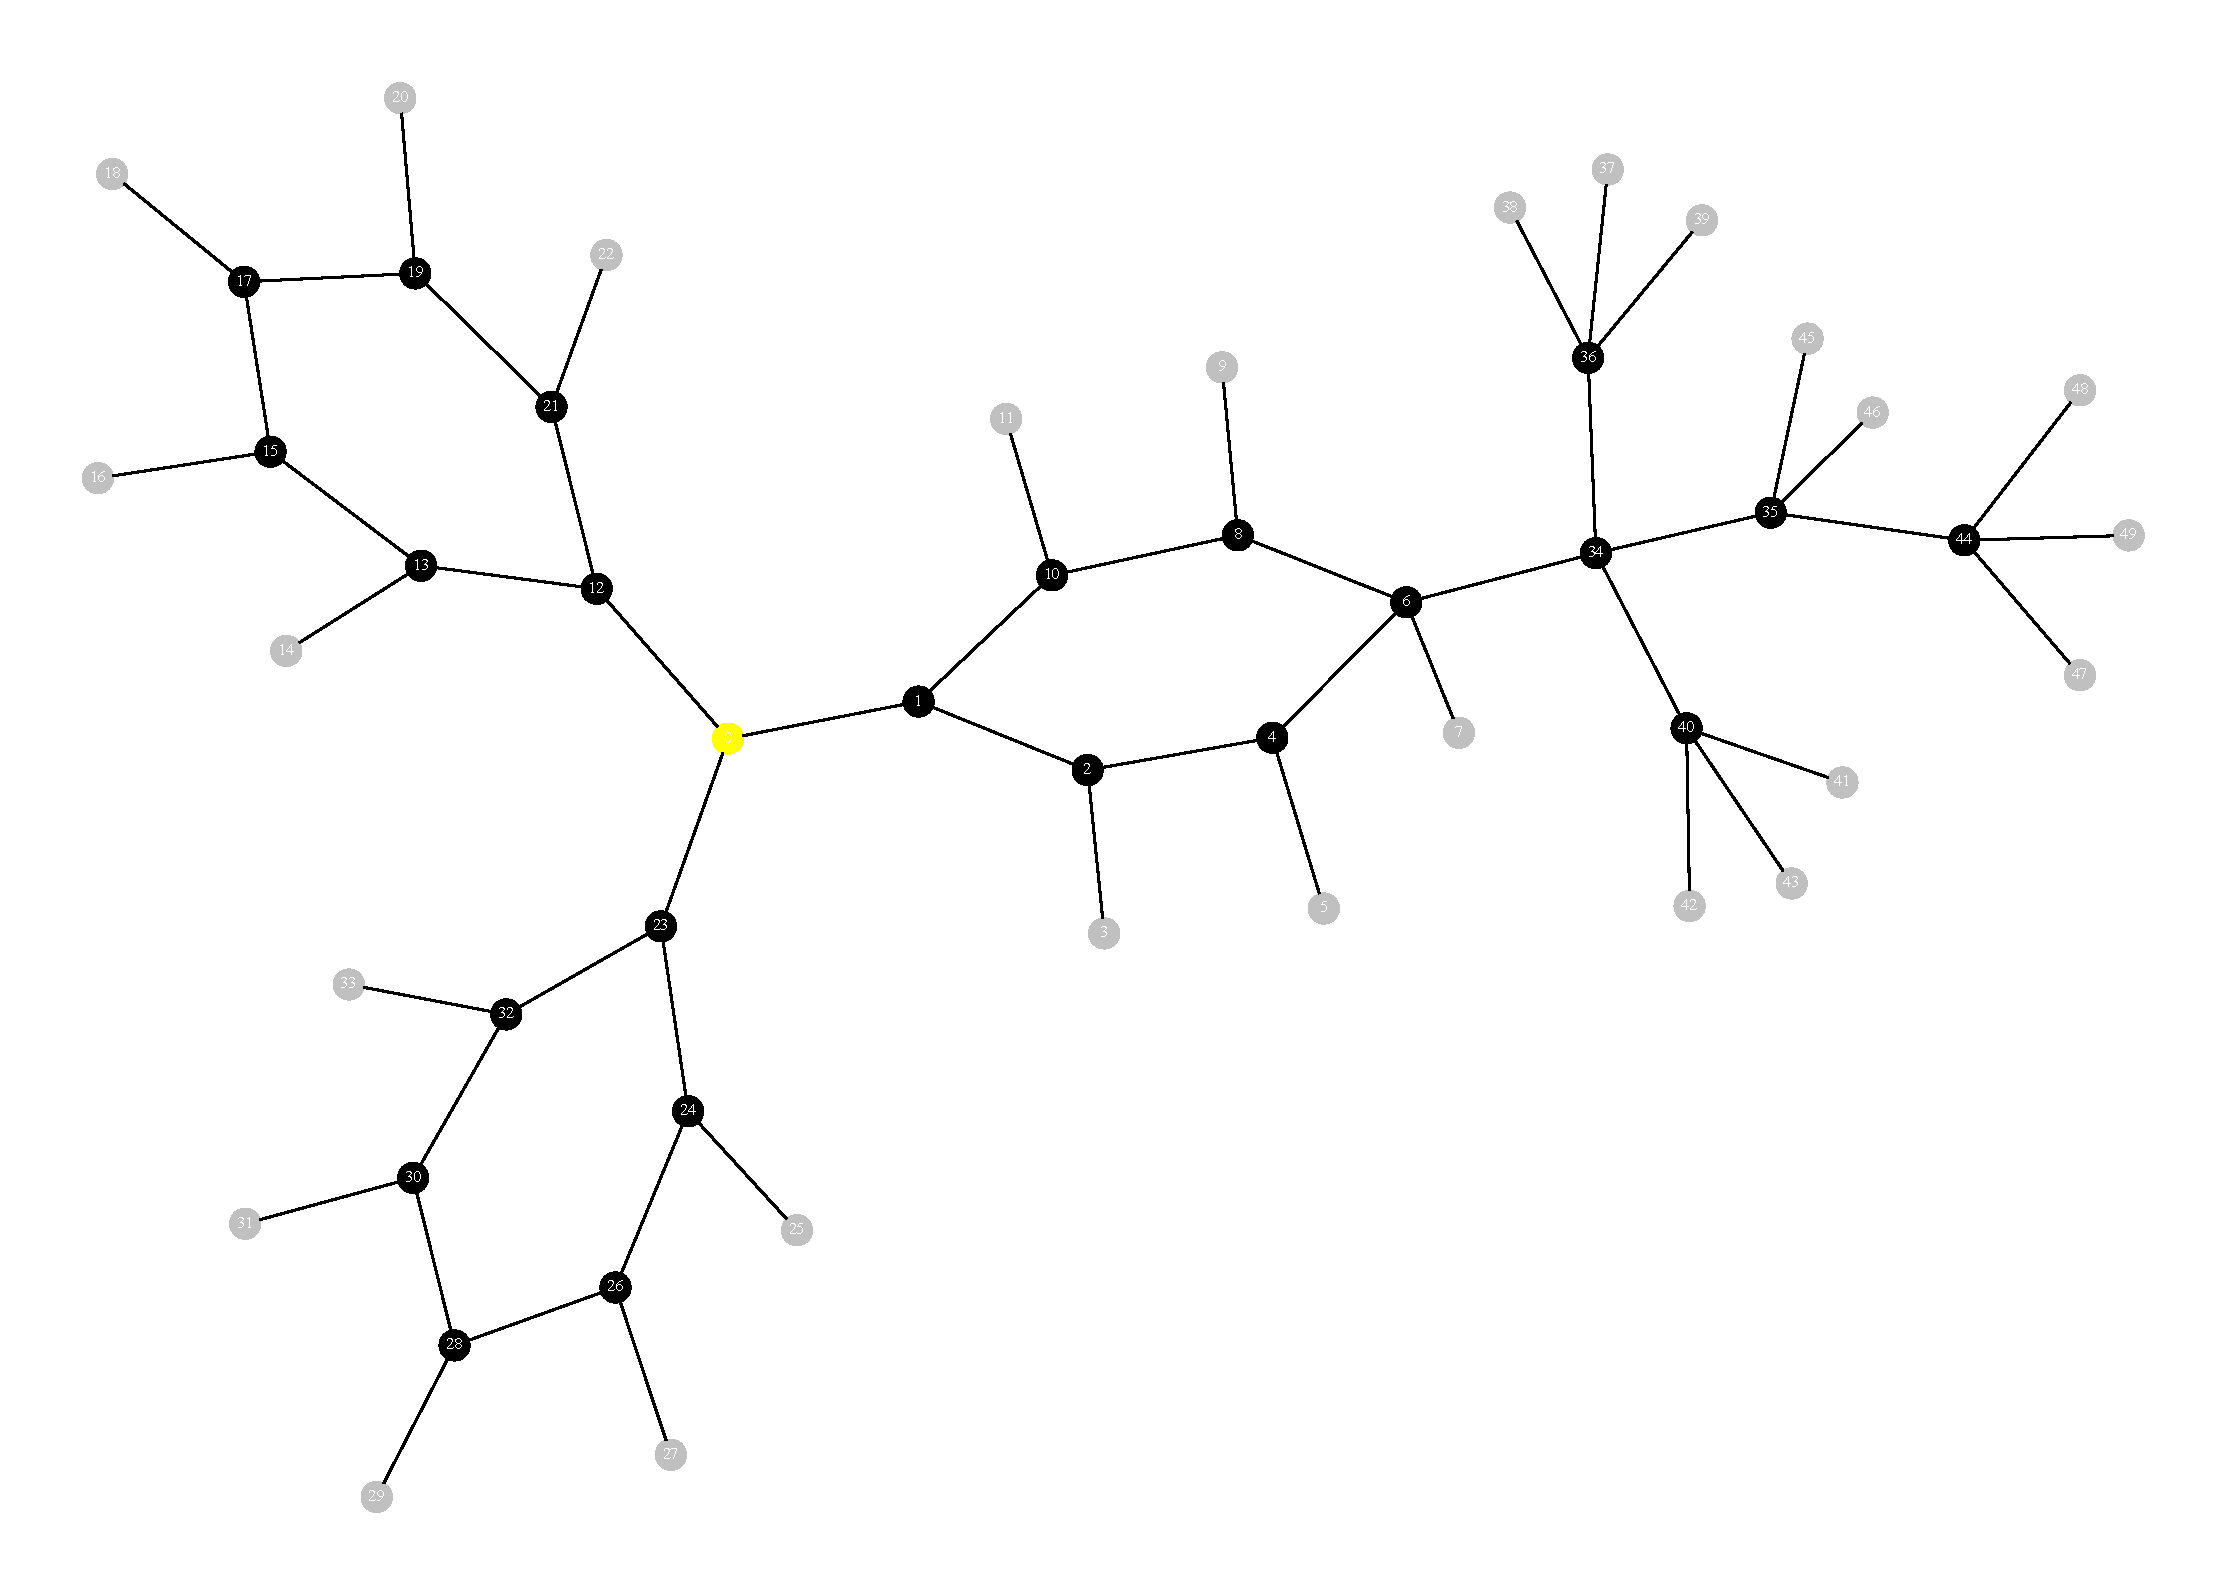
\includegraphics[scale=0.15]{mol_pictures_unfiltered/36.pdf}}

\vspace{1cm}
\begin{verbatim}
<HiPRGen.species_questions.species_default_true object at 0x2b667d6b2430>
Terminal.KEEP
\end{verbatim}


number: 37



entry id: aa3de124b222759aaea1463f6143873b-C23H26S1-0-1



uncorrected free energy: -35095.16063362286



formula: C23 H26 S1

\raisebox{-.5\height}{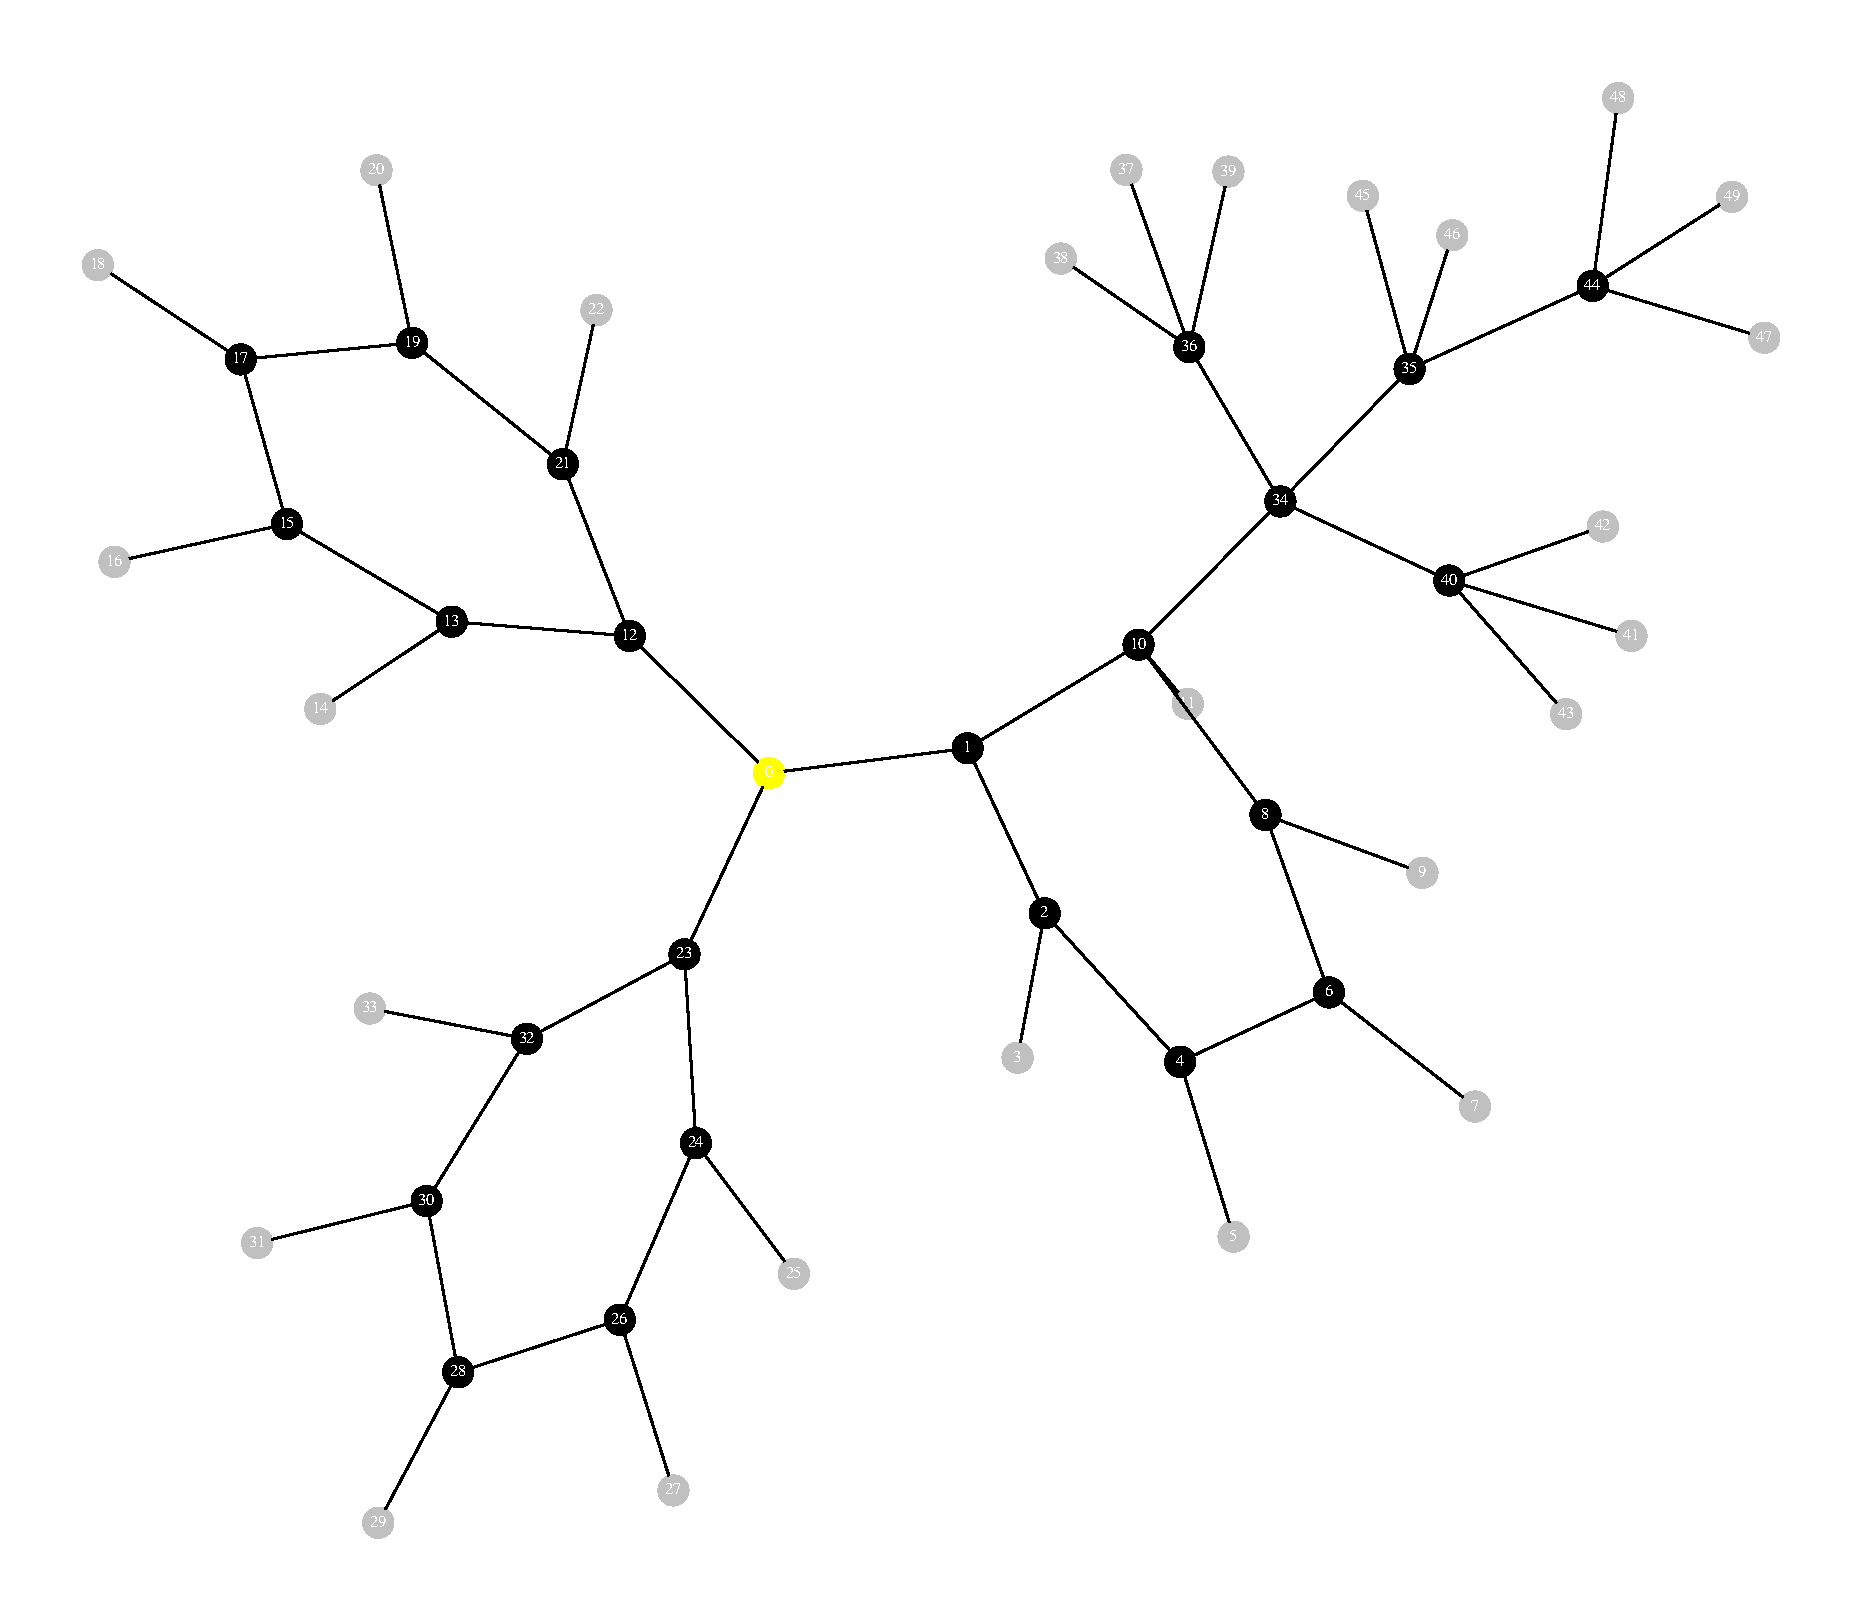
\includegraphics[scale=0.15]{mol_pictures_unfiltered/37.pdf}}

\vspace{1cm}
\begin{verbatim}
<HiPRGen.species_questions.species_default_true object at 0x2b667d6b2430>
Terminal.KEEP
\end{verbatim}


number: 38



entry id: b1540153219ab9844a80bc3ef4d5b560-C23H26S1-1-2



uncorrected free energy: -35090.75581420064



formula: C23 H26 S1

\raisebox{-.5\height}{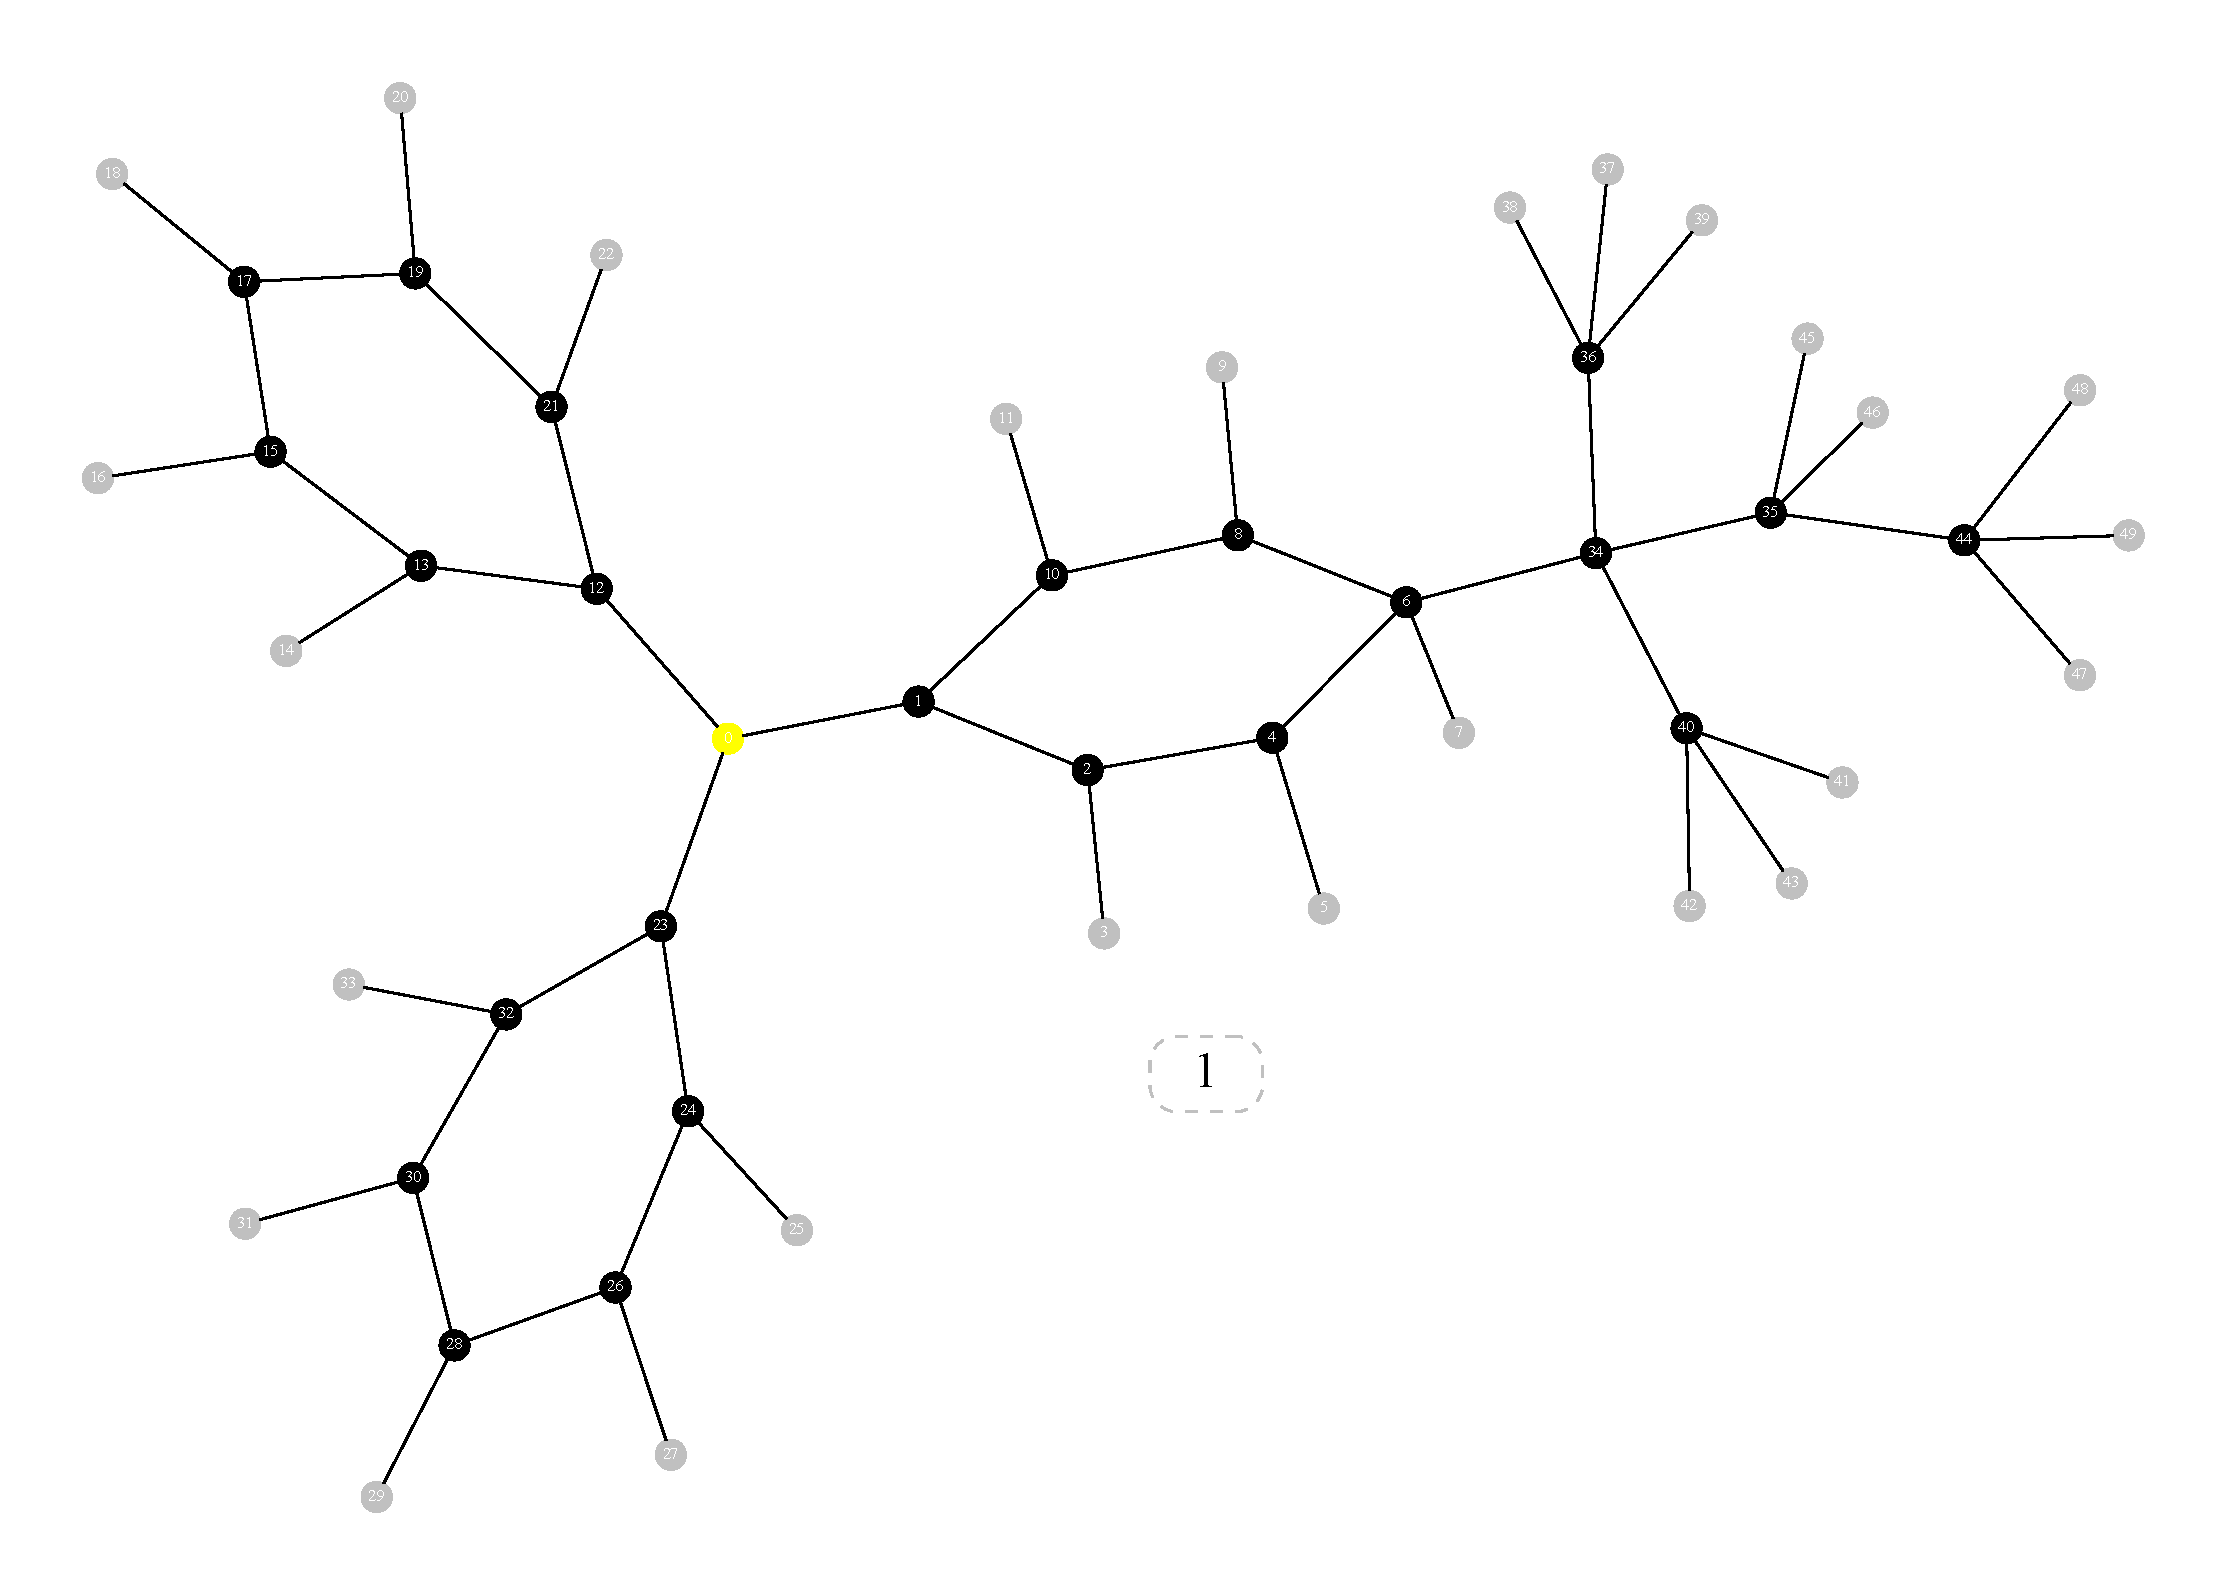
\includegraphics[scale=0.15]{mol_pictures_unfiltered/38.pdf}}

\vspace{1cm}
\begin{verbatim}
<HiPRGen.species_questions.species_default_true object at 0x2b667d6b2430>
Terminal.KEEP
\end{verbatim}


number: 39



entry id: 4e5d4774df9d01e93db3763faa6e7914-C23H26S1-1-2



uncorrected free energy: -35090.36948689221



formula: C23 H26 S1

\raisebox{-.5\height}{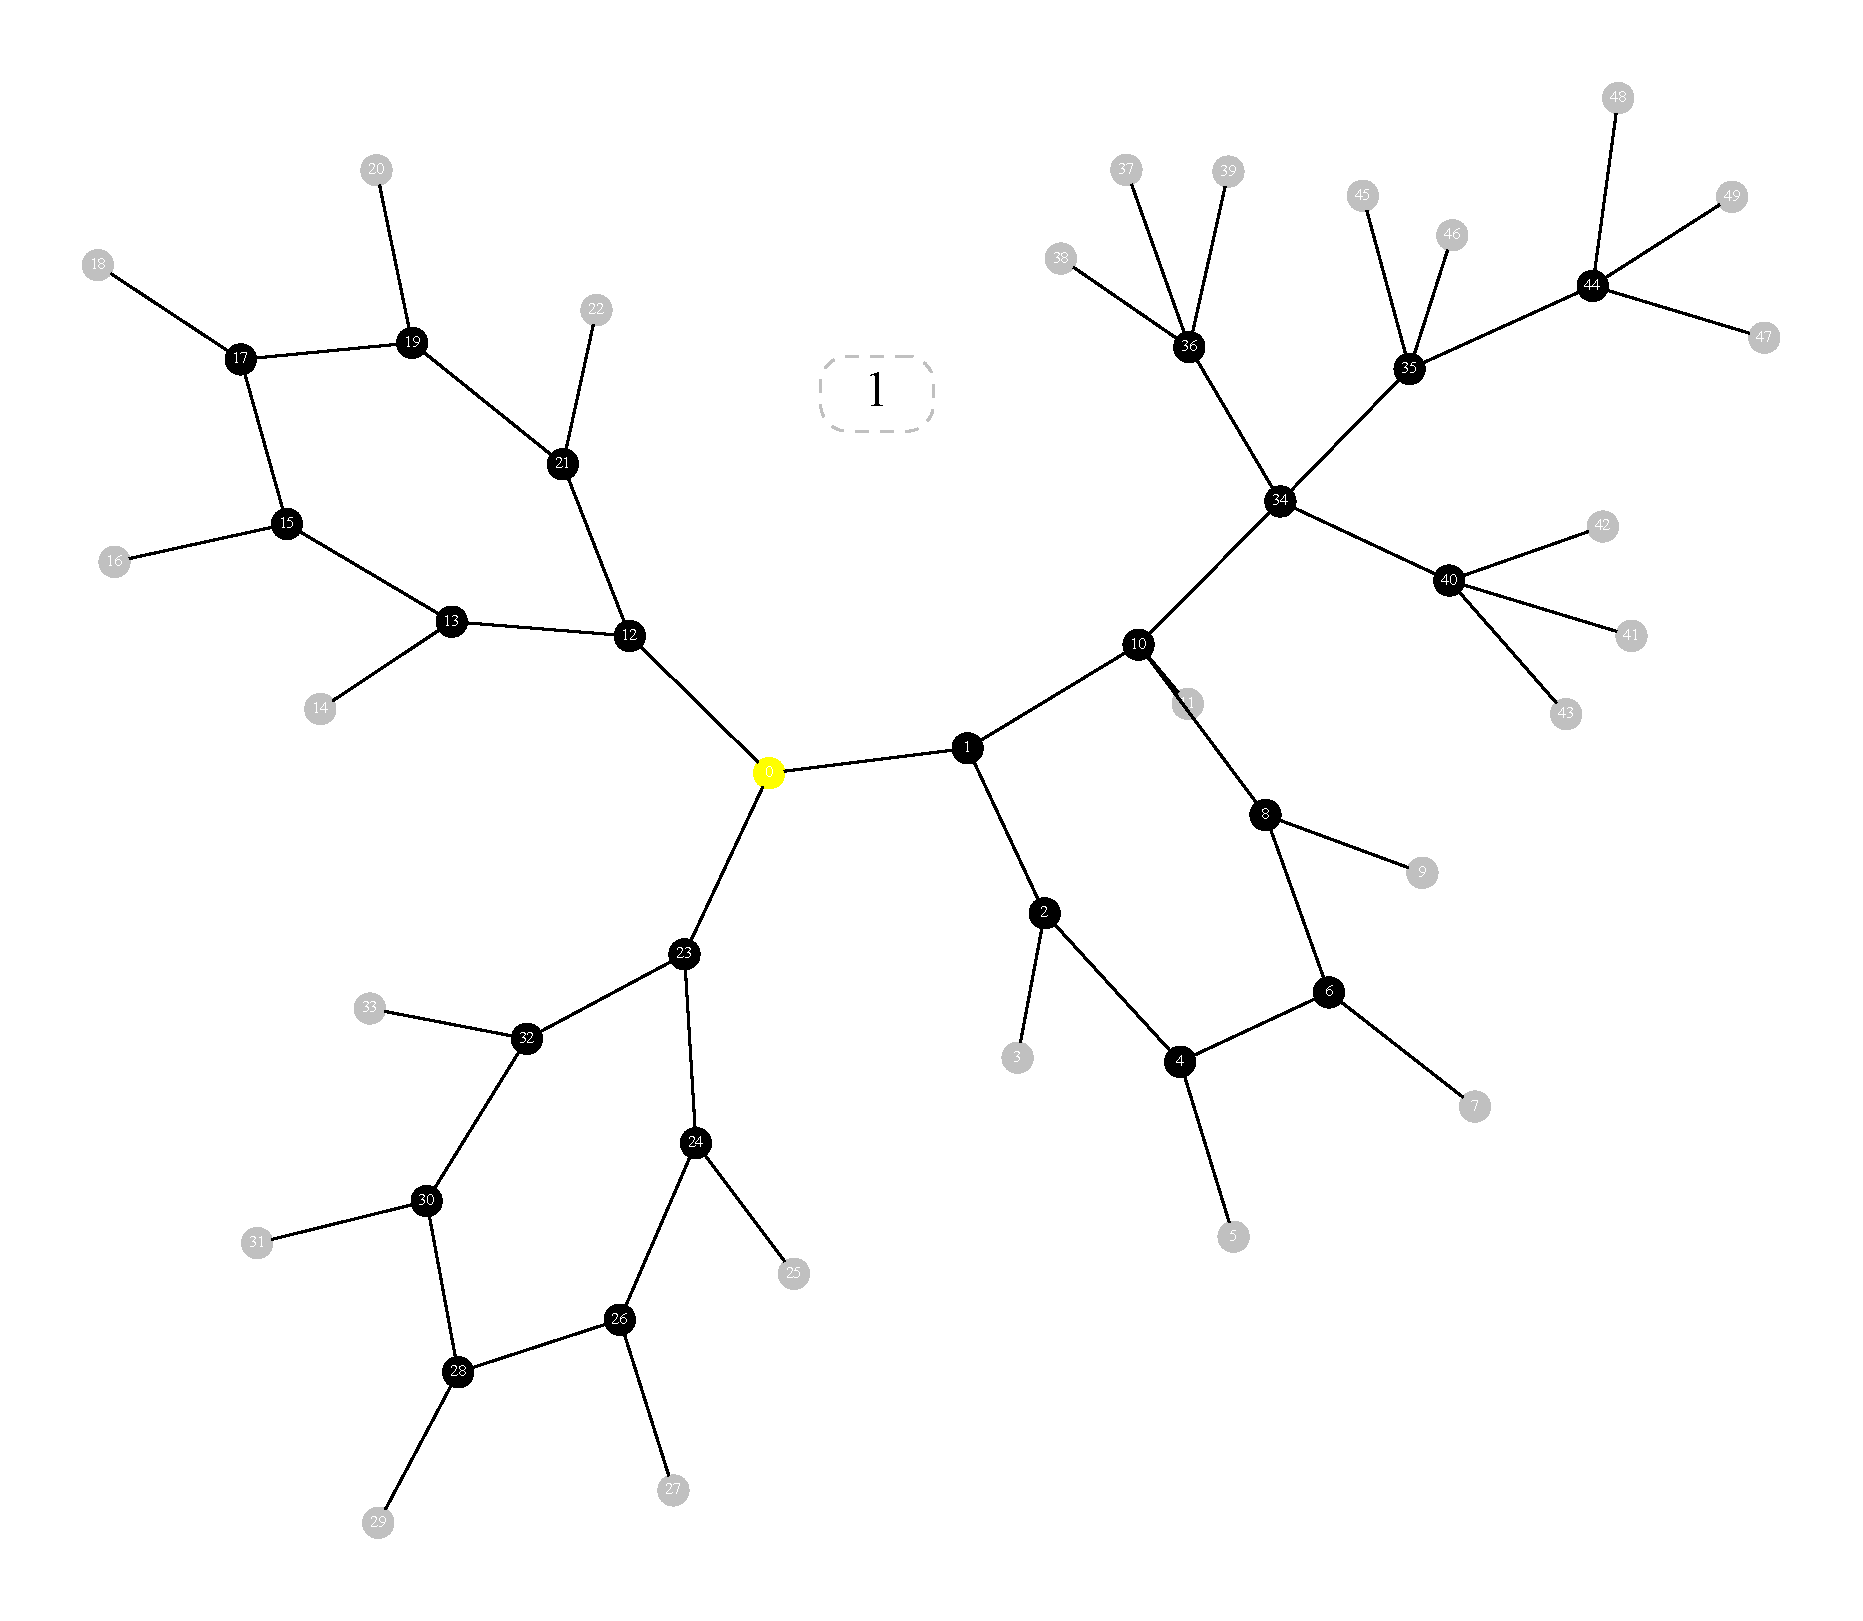
\includegraphics[scale=0.15]{mol_pictures_unfiltered/39.pdf}}

\vspace{1cm}
\begin{verbatim}
<HiPRGen.species_questions.species_default_true object at 0x2b667d6b2430>
Terminal.KEEP
\end{verbatim}


number: 40



entry id: 443639a41f47d07b41b9f1b4150e7e7b-C10H15O1-m1-1



uncorrected free energy: -12656.20077055078



formula: C10 H15 O1

\raisebox{-.5\height}{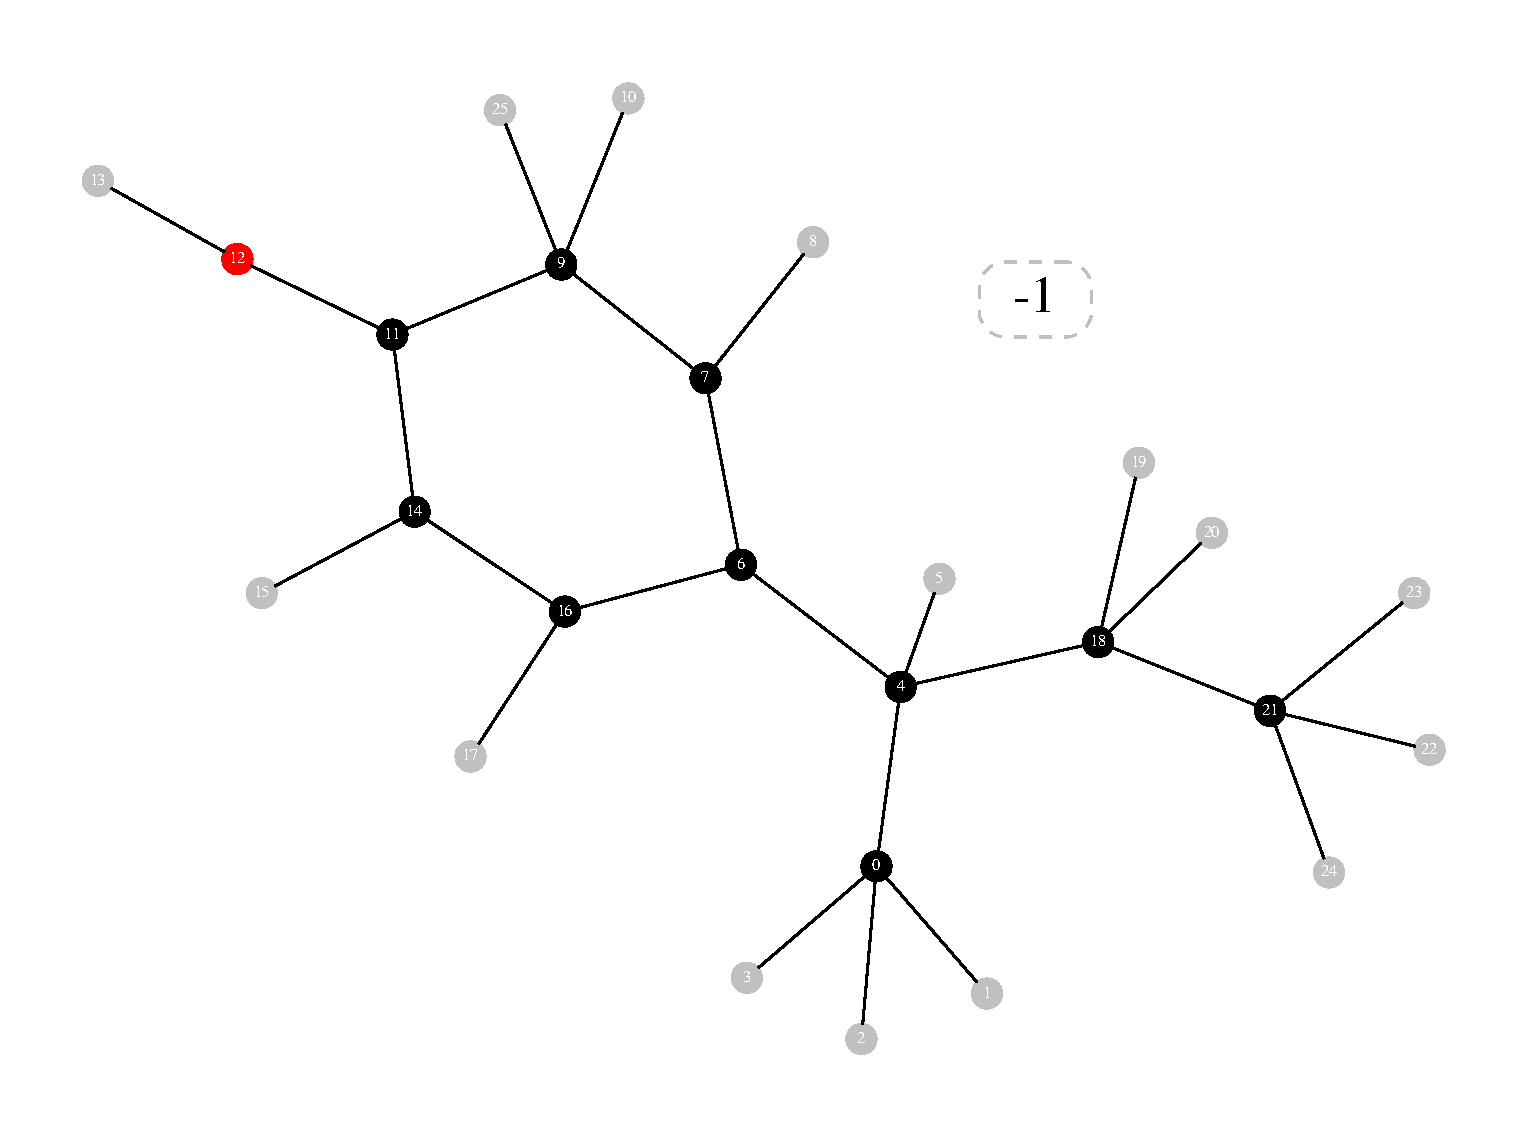
\includegraphics[scale=0.15]{mol_pictures_unfiltered/40.pdf}}

\vspace{1cm}
\begin{verbatim}
<HiPRGen.species_questions.species_default_true object at 0x2b667d6b2430>
Terminal.KEEP
\end{verbatim}


number: 41



entry id: 3adeb22f2907b178f6b106fc59646ad1-C10H15O1-0-2



uncorrected free energy: -12654.411933632726



formula: C10 H15 O1

\raisebox{-.5\height}{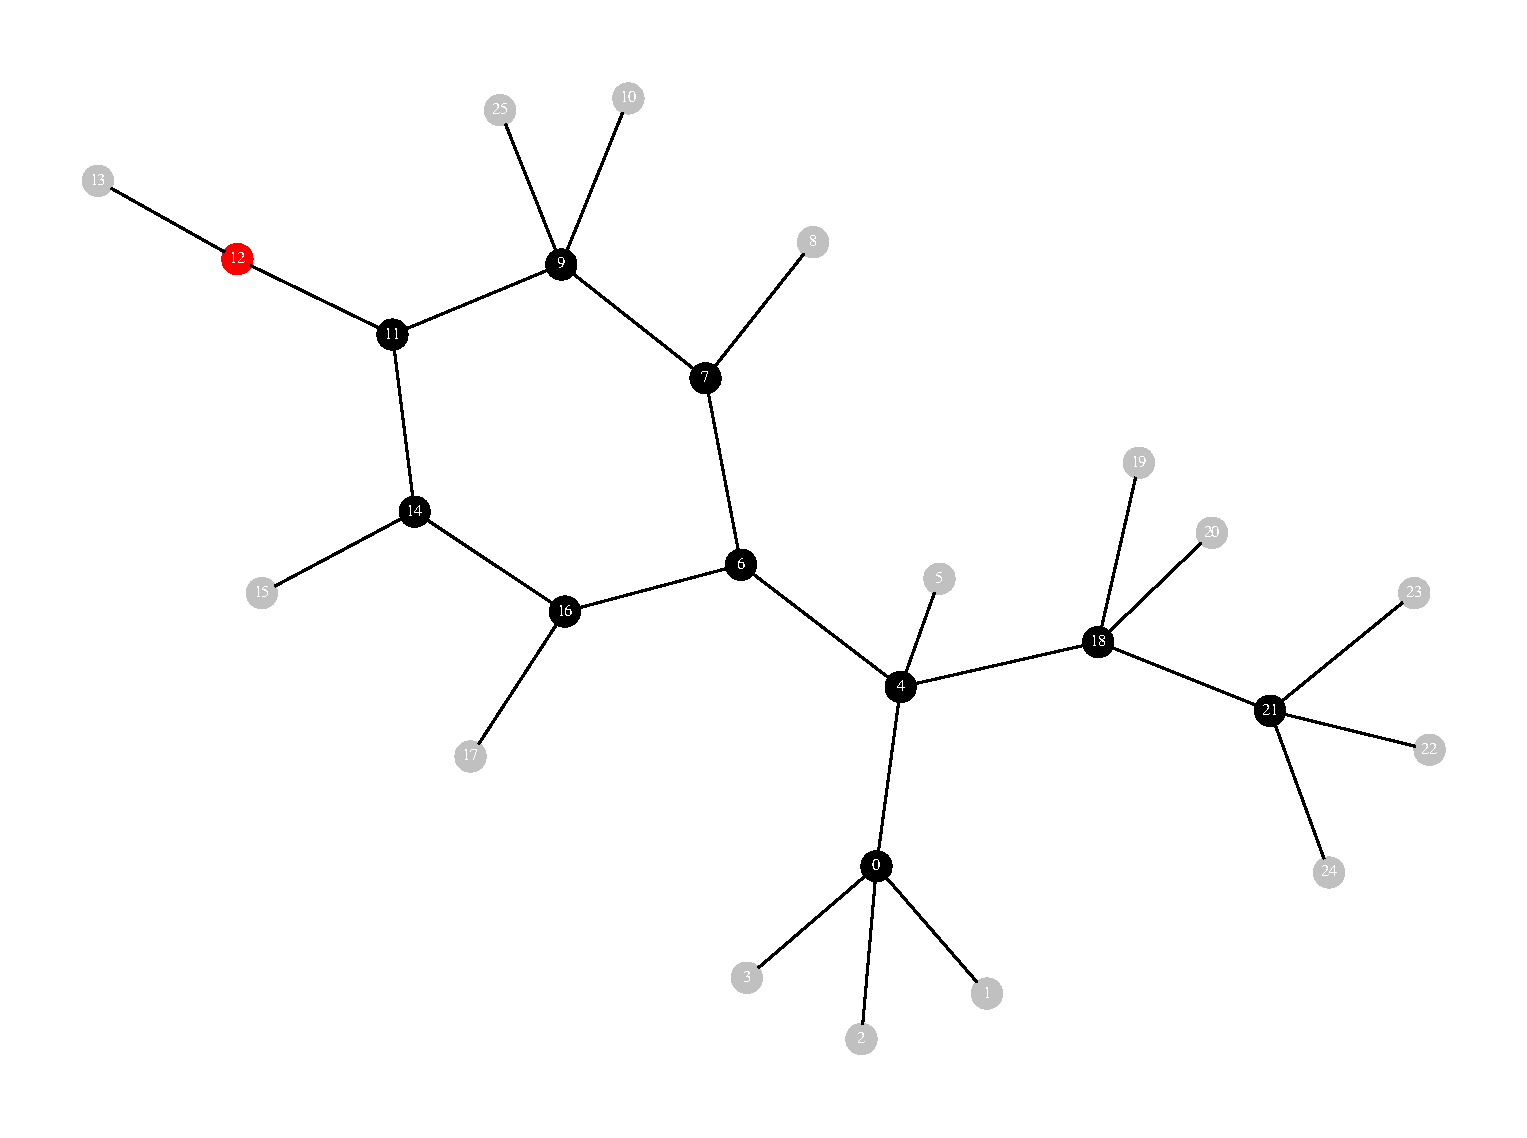
\includegraphics[scale=0.15]{mol_pictures_unfiltered/41.pdf}}

\vspace{1cm}
\begin{verbatim}
<HiPRGen.species_questions.species_default_true object at 0x2b667d6b2430>
Terminal.KEEP
\end{verbatim}


number: 42



entry id: 3222ddd6de9a68c13c9a14952aabf24e-C10H15O1-1-1



uncorrected free energy: -12649.646675455047



formula: C10 H15 O1

\raisebox{-.5\height}{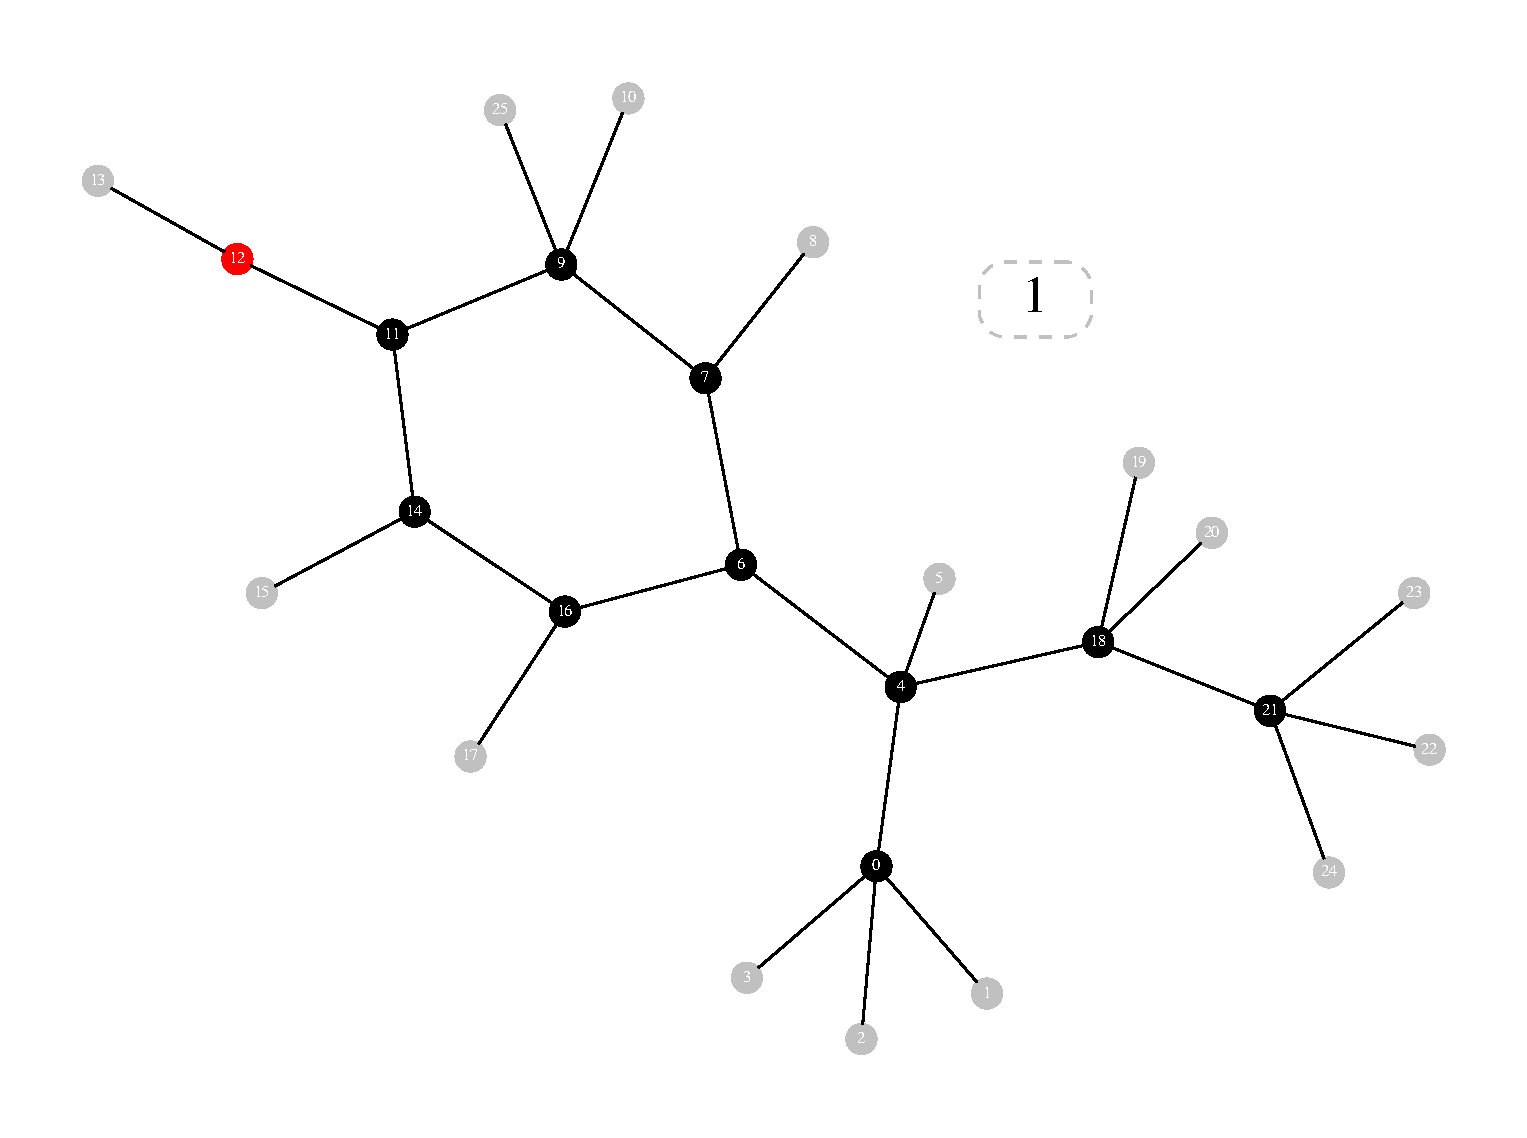
\includegraphics[scale=0.15]{mol_pictures_unfiltered/42.pdf}}

\vspace{1cm}
\begin{verbatim}
<HiPRGen.species_questions.species_default_true object at 0x2b667d6b2430>
Terminal.KEEP
\end{verbatim}


number: 43



entry id: 7365841bed8fe73e132c46960e8c23e4-H2O1-m1-2



uncorrected free energy: -2079.9357742987468



formula: H2 O1

\raisebox{-.5\height}{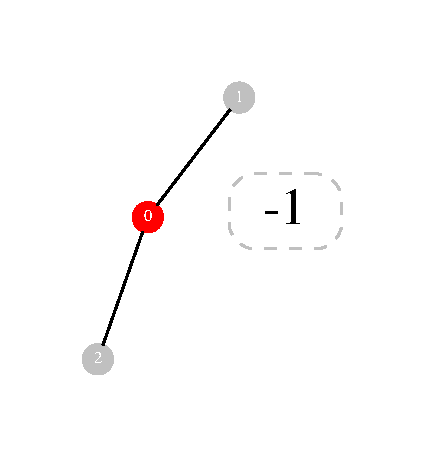
\includegraphics[scale=0.15]{mol_pictures_unfiltered/43.pdf}}

\vspace{1cm}
\begin{verbatim}
<HiPRGen.species_questions.species_default_true object at 0x2b667d6b2430>
Terminal.KEEP
\end{verbatim}


number: 44



entry id: aab0ea89ff9b4e27da78126a6c80cbf0-H2O1-0-1



uncorrected free energy: -2079.873783910513



formula: H2 O1

\raisebox{-.5\height}{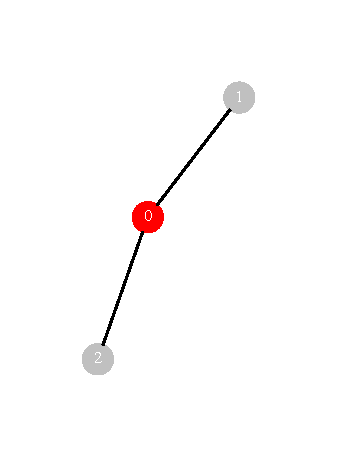
\includegraphics[scale=0.15]{mol_pictures_unfiltered/44.pdf}}

\vspace{1cm}
\begin{verbatim}
<HiPRGen.species_questions.species_default_true object at 0x2b667d6b2430>
Terminal.KEEP
\end{verbatim}


number: 45



entry id: f157c4b8fe094772f3a425e5dfc57294-H2O1-1-2



uncorrected free energy: -2069.641064122109



formula: H2 O1

\raisebox{-.5\height}{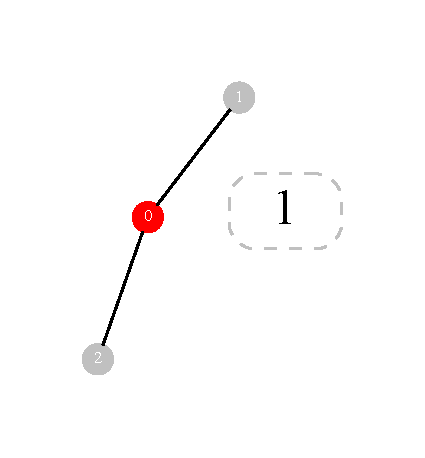
\includegraphics[scale=0.15]{mol_pictures_unfiltered/45.pdf}}

\vspace{1cm}
\begin{verbatim}
<HiPRGen.species_questions.species_default_true object at 0x2b667d6b2430>
Terminal.KEEP
\end{verbatim}


number: 46



entry id: a9e891e561bce34cf4b49b6c7c2347c6-C6H11O2-m1-1



uncorrected free energy: -10495.525058434632



formula: C6 H11 O2

\raisebox{-.5\height}{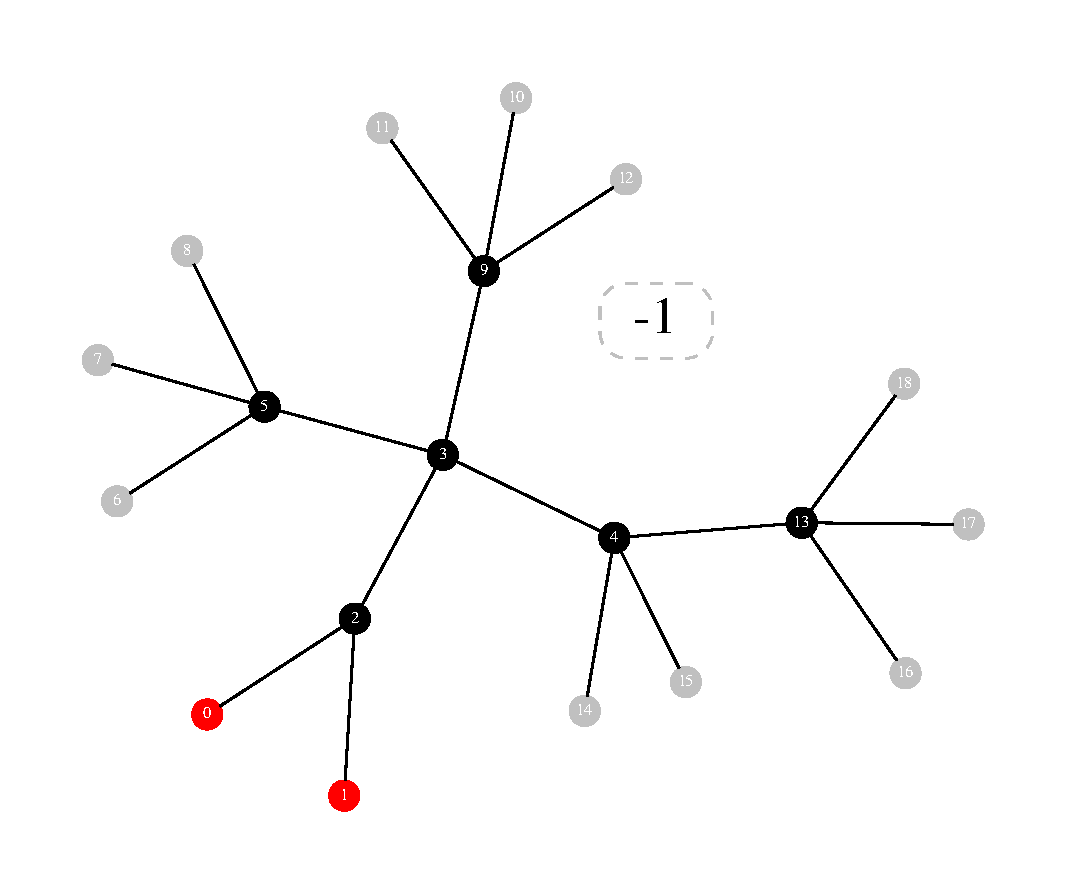
\includegraphics[scale=0.15]{mol_pictures_unfiltered/46.pdf}}

\vspace{1cm}
\begin{verbatim}
<HiPRGen.species_questions.species_default_true object at 0x2b667d6b2430>
Terminal.KEEP
\end{verbatim}


number: 47



entry id: 0701a0edad7058c8168456de1c92e8e0-C6H11O2-0-2



uncorrected free energy: -10490.532211506848



formula: C6 H11 O2

\raisebox{-.5\height}{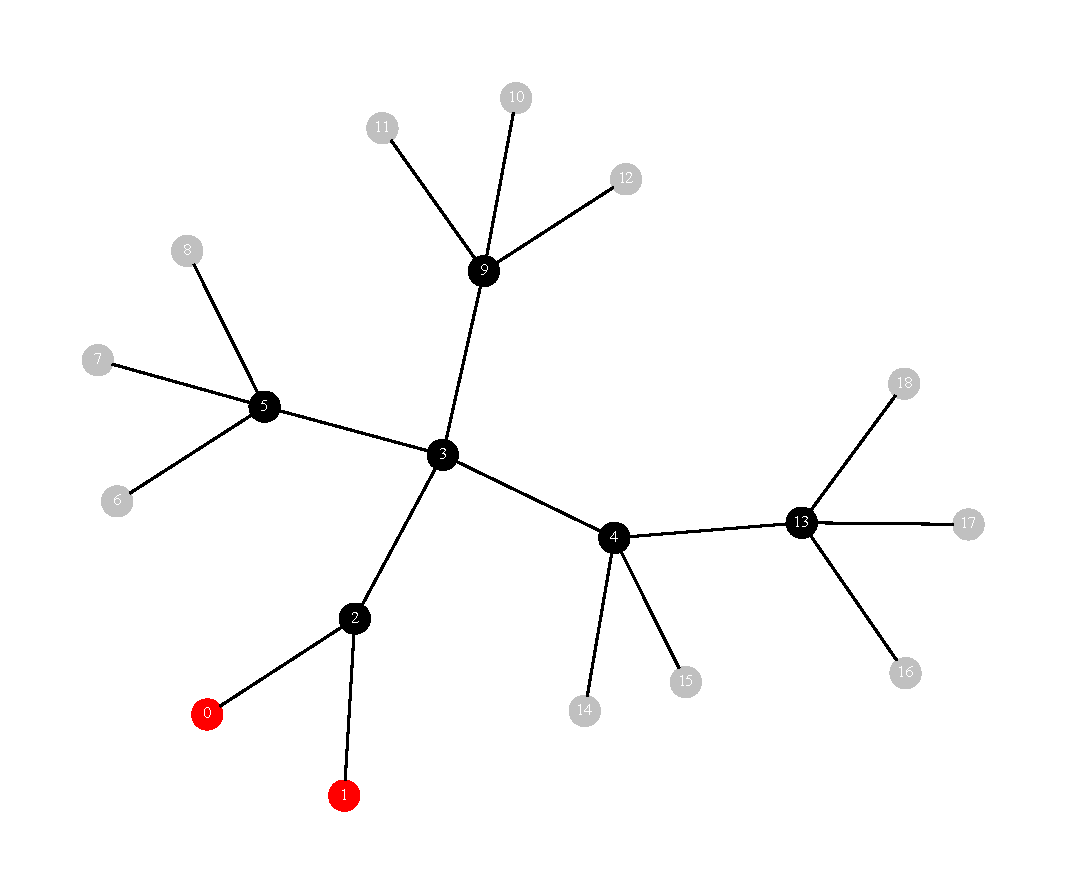
\includegraphics[scale=0.15]{mol_pictures_unfiltered/47.pdf}}

\vspace{1cm}
\begin{verbatim}
<HiPRGen.species_questions.species_default_true object at 0x2b667d6b2430>
Terminal.KEEP
\end{verbatim}


number: 48



entry id: a7acbdb77305196bf789ae0c875d0f19-C6H5-m1-1



uncorrected free energy: -6301.668558148871



formula: C6 H5

\raisebox{-.5\height}{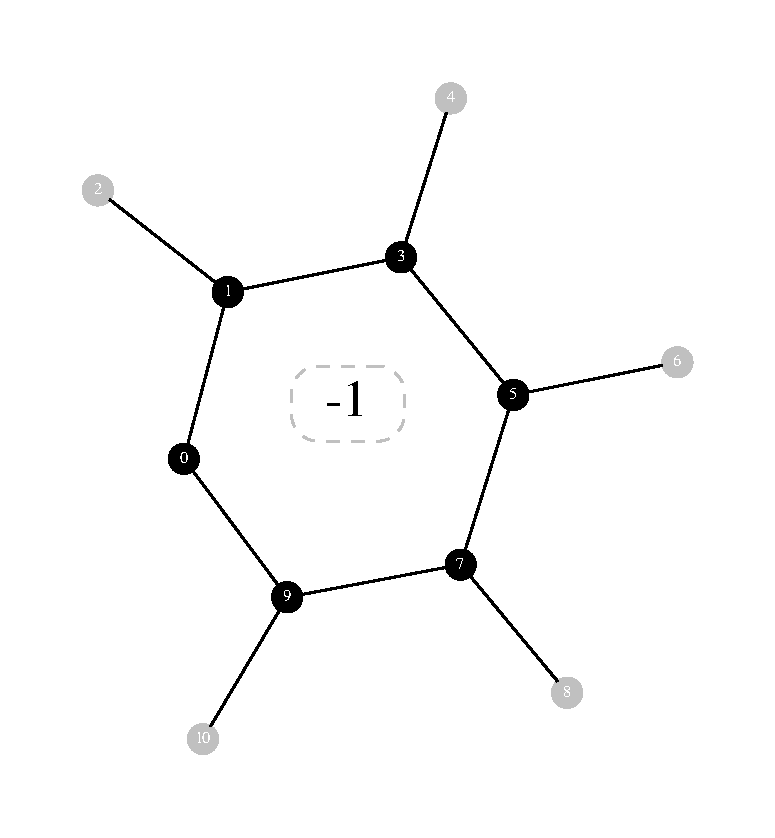
\includegraphics[scale=0.15]{mol_pictures_unfiltered/48.pdf}}

\vspace{1cm}
\begin{verbatim}
<HiPRGen.species_questions.species_default_true object at 0x2b667d6b2430>
Terminal.KEEP
\end{verbatim}


number: 49



entry id: c9636169ed9efe63dd613dad22c5b63f-C6H5-0-2



uncorrected free energy: -6298.918176108165



formula: C6 H5

\raisebox{-.5\height}{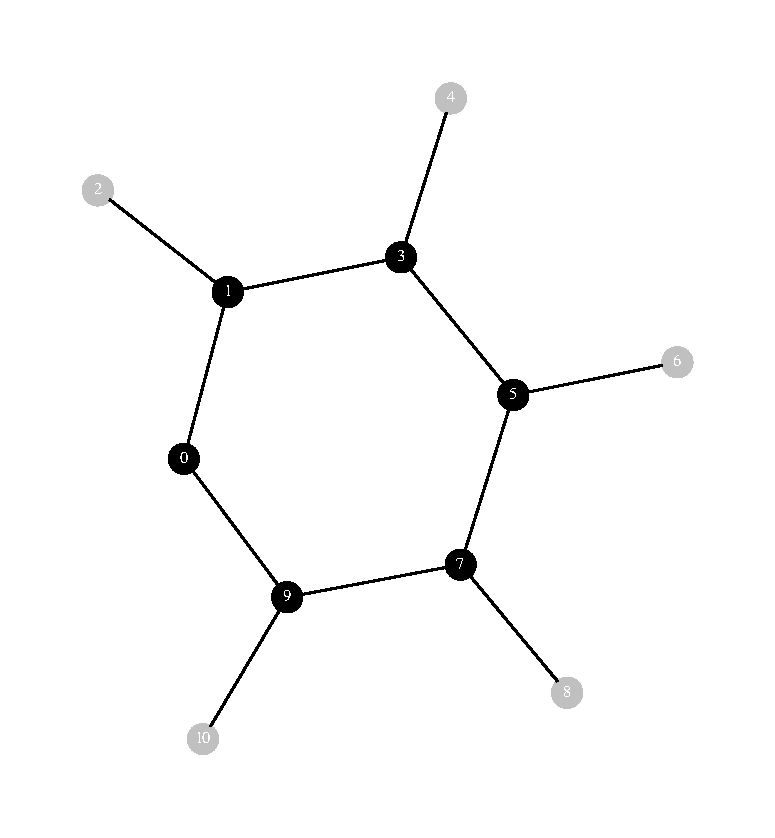
\includegraphics[scale=0.15]{mol_pictures_unfiltered/49.pdf}}

\vspace{1cm}
\begin{verbatim}
<HiPRGen.species_questions.species_default_true object at 0x2b667d6b2430>
Terminal.KEEP
\end{verbatim}


number: 50



entry id: ace426ad373f83a93c83458cf66b8866-C6H5-1-1



uncorrected free energy: -6292.336186550749



formula: C6 H5

\raisebox{-.5\height}{\includegraphics[scale=0.15]{mol_pictures_unfiltered/50.pdf}}

\vspace{1cm}
\begin{verbatim}
<HiPRGen.species_questions.species_default_true object at 0x2b667d6b2430>
Terminal.KEEP
\end{verbatim}


number: 51



entry id: bf845e308e61c1f4aeb1392daf2af740-C13H13S1-m1-1



uncorrected free energy: -24522.92145073565



formula: C13 H13 S1

\raisebox{-.5\height}{\includegraphics[scale=0.15]{mol_pictures_unfiltered/51.pdf}}

\vspace{1cm}
\begin{verbatim}
<HiPRGen.species_questions.species_default_true object at 0x2b667d6b2430>
Terminal.KEEP
\end{verbatim}


number: 52



entry id: 60e63c69581d9af4f0f33039786cea50-C13H13S1-0-2



uncorrected free energy: -24520.406660494013



formula: C13 H13 S1

\raisebox{-.5\height}{\includegraphics[scale=0.15]{mol_pictures_unfiltered/52.pdf}}

\vspace{1cm}
\begin{verbatim}
<HiPRGen.species_questions.species_default_true object at 0x2b667d6b2430>
Terminal.KEEP
\end{verbatim}


number: 53



entry id: 3bd4ab1135b39ff25d94beb51dd6c503-C13H13S1-1-1



uncorrected free energy: -24515.459113537858



formula: C13 H13 S1

\raisebox{-.5\height}{\includegraphics[scale=0.15]{mol_pictures_unfiltered/53.pdf}}

\vspace{1cm}
\begin{verbatim}
<HiPRGen.species_questions.species_default_true object at 0x2b667d6b2430>
Terminal.KEEP
\end{verbatim}


number: 54



entry id: 3ce8bce066bf652195a8784f7b4f04af-C10H19O2-0-2



uncorrected free energy: -14765.933688558556



formula: C10 H19 O2

\raisebox{-.5\height}{\includegraphics[scale=0.15]{mol_pictures_unfiltered/54.pdf}}

\vspace{1cm}
\begin{verbatim}
<HiPRGen.species_questions.species_default_true object at 0x2b667d6b2430>
Terminal.KEEP
\end{verbatim}


number: 55



entry id: fb79683b7f312a9cf81ffef86594feba-C1H3-m1-1



uncorrected free energy: -1085.1504582113405



formula: C1 H3

\raisebox{-.5\height}{\includegraphics[scale=0.15]{mol_pictures_unfiltered/55.pdf}}

\vspace{1cm}
\begin{verbatim}
<HiPRGen.species_questions.species_default_true object at 0x2b667d6b2430>
Terminal.KEEP
\end{verbatim}


number: 56



entry id: 5f85470c393edc87393085bba5b03428-C1H3-0-2



uncorrected free energy: -1083.2057568833218



formula: C1 H3

\raisebox{-.5\height}{\includegraphics[scale=0.15]{mol_pictures_unfiltered/56.pdf}}

\vspace{1cm}
\begin{verbatim}
<HiPRGen.species_questions.species_default_true object at 0x2b667d6b2430>
Terminal.KEEP
\end{verbatim}


number: 57



entry id: cb48ad765690f27a672c38acf77f12c2-C1H3-1-1



uncorrected free energy: -1075.5798123450227



formula: C1 H3

\raisebox{-.5\height}{\includegraphics[scale=0.15]{mol_pictures_unfiltered/57.pdf}}

\vspace{1cm}
\begin{verbatim}
<HiPRGen.species_questions.species_default_true object at 0x2b667d6b2430>
Terminal.KEEP
\end{verbatim}


number: 58



entry id: 6203000256b3f131b82ca6c273f2fe5d-C10H13-m1-1



uncorrected free energy: -10577.002303712354



formula: C10 H13

\raisebox{-.5\height}{\includegraphics[scale=0.15]{mol_pictures_unfiltered/58.pdf}}

\vspace{1cm}
\begin{verbatim}
<HiPRGen.species_questions.species_default_true object at 0x2b667d6b2430>
Terminal.KEEP
\end{verbatim}


number: 59



entry id: 82ca46cecd8439a6d7fbd87eea2c54b9-C10H13-0-2



uncorrected free energy: -10574.252479640065



formula: C10 H13

\raisebox{-.5\height}{\includegraphics[scale=0.15]{mol_pictures_unfiltered/59.pdf}}

\vspace{1cm}
\begin{verbatim}
<HiPRGen.species_questions.species_default_true object at 0x2b667d6b2430>
Terminal.KEEP
\end{verbatim}


number: 60



entry id: 705bbb0e5307bd961891ae2334cee3dc-C10H13-1-1



uncorrected free energy: -10567.753851087275



formula: C10 H13

\raisebox{-.5\height}{\includegraphics[scale=0.15]{mol_pictures_unfiltered/60.pdf}}

\vspace{1cm}
\begin{verbatim}
<HiPRGen.species_questions.species_default_true object at 0x2b667d6b2430>
Terminal.KEEP
\end{verbatim}


number: 61



entry id: 31c2af8f1605817c400250991fe7fefe-C4F9H1O3S1-0-1



uncorrected free energy: -45596.45874412551



formula: C4 F9 H1 O3 S1

\raisebox{-.5\height}{\includegraphics[scale=0.15]{mol_pictures_unfiltered/61.pdf}}

\vspace{1cm}
\begin{verbatim}
<HiPRGen.species_questions.species_default_true object at 0x2b667d6b2430>
Terminal.KEEP
\end{verbatim}


number: 62



entry id: 2699beb3fcbcc2b0075c9dd8f7b304cb-C6H12O1-m1-2



uncorrected free energy: -8461.167846444436



formula: C6 H12 O1

\raisebox{-.5\height}{\includegraphics[scale=0.15]{mol_pictures_unfiltered/62.pdf}}

\vspace{1cm}
\begin{verbatim}
<HiPRGen.species_questions.species_default_true object at 0x2b667d6b2430>
Terminal.KEEP
\end{verbatim}


number: 63



entry id: 3464f250ed90621ea6a9588d1705d205-C6H12O1-0-1



uncorrected free energy: -8460.378491681187



formula: C6 H12 O1

\raisebox{-.5\height}{\includegraphics[scale=0.15]{mol_pictures_unfiltered/63.pdf}}

\vspace{1cm}
\begin{verbatim}
<HiPRGen.species_questions.species_default_true object at 0x2b667d6b2430>
Terminal.KEEP
\end{verbatim}


number: 64



entry id: 86511bda5d0f000e5685e9c2e9e7be53-C6H12O1-1-2



uncorrected free energy: -8452.458390250442



formula: C6 H12 O1

\raisebox{-.5\height}{\includegraphics[scale=0.15]{mol_pictures_unfiltered/64.pdf}}

\vspace{1cm}
\begin{verbatim}
<HiPRGen.species_questions.species_default_true object at 0x2b667d6b2430>
Terminal.KEEP
\end{verbatim}


number: 65



entry id: 7d4d03d7557395fd35364ec1cfc6add2-C10H14O1-m1-2



uncorrected free energy: -12640.406719740313



formula: C10 H14 O1

\raisebox{-.5\height}{\includegraphics[scale=0.15]{mol_pictures_unfiltered/65.pdf}}

\vspace{1cm}
\begin{verbatim}
<HiPRGen.species_questions.species_default_true object at 0x2b667d6b2430>
Terminal.KEEP
\end{verbatim}


number: 66



entry id: 8b8c577519e77347f52c970bc6f2bcdd-C10H14O1-m1-2



uncorrected free energy: -12641.256465891402



formula: C10 H14 O1

\raisebox{-.5\height}{\includegraphics[scale=0.15]{mol_pictures_unfiltered/66.pdf}}

\vspace{1cm}
\begin{verbatim}
<HiPRGen.species_questions.species_default_true object at 0x2b667d6b2430>
Terminal.KEEP
\end{verbatim}


number: 67



entry id: 1d64d1a96b5db50b9fdf583dc18f90cf-C10H14O1-0-1



uncorrected free energy: -12639.959950636323



formula: C10 H14 O1

\raisebox{-.5\height}{\includegraphics[scale=0.15]{mol_pictures_unfiltered/67.pdf}}

\vspace{1cm}
\begin{verbatim}
<HiPRGen.species_questions.species_default_true object at 0x2b667d6b2430>
Terminal.KEEP
\end{verbatim}


number: 68



entry id: 62e08d5119480b03357cc679f310168d-C10H14O1-0-1



uncorrected free energy: -12639.27597622435



formula: C10 H14 O1

\raisebox{-.5\height}{\includegraphics[scale=0.15]{mol_pictures_unfiltered/68.pdf}}

\vspace{1cm}
\begin{verbatim}
<HiPRGen.species_questions.species_default_true object at 0x2b667d6b2430>
Terminal.KEEP
\end{verbatim}


number: 69



entry id: e9382c788338f71391524d940b96d69e-C10H14O1-1-2



uncorrected free energy: -12633.32607140473



formula: C10 H14 O1

\raisebox{-.5\height}{\includegraphics[scale=0.15]{mol_pictures_unfiltered/69.pdf}}

\vspace{1cm}
\begin{verbatim}
<HiPRGen.species_questions.species_default_true object at 0x2b667d6b2430>
Terminal.KEEP
\end{verbatim}


number: 70



entry id: b1d9b641790ab43d18cb8d4637b7fae0-C10H14O1-1-2



uncorrected free energy: -12632.159367732



formula: C10 H14 O1

\raisebox{-.5\height}{\includegraphics[scale=0.15]{mol_pictures_unfiltered/70.pdf}}

\vspace{1cm}
\begin{verbatim}
<HiPRGen.species_questions.species_default_true object at 0x2b667d6b2430>
Terminal.KEEP
\end{verbatim}


number: 71



entry id: baa58da5bef49709d3547c41ce3f3b80-C10H20O2-m1-2



uncorrected free energy: -14784.023911463151



formula: C10 H20 O2

\raisebox{-.5\height}{\includegraphics[scale=0.15]{mol_pictures_unfiltered/71.pdf}}

\vspace{1cm}
\begin{verbatim}
<HiPRGen.species_questions.species_default_true object at 0x2b667d6b2430>
Terminal.KEEP
\end{verbatim}


number: 72



entry id: 0aade5ee5263fd1ad77490688fb37d0e-C10H20O2-0-1



uncorrected free energy: -14783.726373365138



formula: C10 H20 O2

\raisebox{-.5\height}{\includegraphics[scale=0.15]{mol_pictures_unfiltered/72.pdf}}

\vspace{1cm}
\begin{verbatim}
<HiPRGen.species_questions.species_default_true object at 0x2b667d6b2430>
Terminal.KEEP
\end{verbatim}


number: 73



entry id: 836983f55a91c9ab5862a0055ec0cfc7-C10H20O2-1-2



uncorrected free energy: -14775.723381925452



formula: C10 H20 O2

\raisebox{-.5\height}{\includegraphics[scale=0.15]{mol_pictures_unfiltered/73.pdf}}

\vspace{1cm}
\begin{verbatim}
<HiPRGen.species_questions.species_default_true object at 0x2b667d6b2430>
Terminal.KEEP
\end{verbatim}


number: 74



entry id: 66beeac3fabe98289969e2e3a67dbb9b-C6H12O2-m1-2



uncorrected free energy: -10508.903171007532



formula: C6 H12 O2

\raisebox{-.5\height}{\includegraphics[scale=0.15]{mol_pictures_unfiltered/74.pdf}}

\vspace{1cm}
\begin{verbatim}
<HiPRGen.species_questions.species_default_true object at 0x2b667d6b2430>
Terminal.KEEP
\end{verbatim}


number: 75



entry id: a4c65f243bb0eef36b5ee0a359560871-C6H12O2-0-1



uncorrected free energy: -10508.508960790188



formula: C6 H12 O2

\raisebox{-.5\height}{\includegraphics[scale=0.15]{mol_pictures_unfiltered/75.pdf}}

\vspace{1cm}
\begin{verbatim}
<HiPRGen.species_questions.species_default_true object at 0x2b667d6b2430>
Terminal.KEEP
\end{verbatim}


number: 76



entry id: 645243313f5f8643fd55474ab64cb472-C6H12O2-1-2



uncorrected free energy: -10500.127095795115



formula: C6 H12 O2

\raisebox{-.5\height}{\includegraphics[scale=0.15]{mol_pictures_unfiltered/76.pdf}}

\vspace{1cm}
\begin{verbatim}
<HiPRGen.species_questions.species_default_true object at 0x2b667d6b2430>
Terminal.KEEP
\end{verbatim}


number: 77



entry id: 4631a22ef2bcb97a654a1c7308b02b01-C18H16S1-m1-2



uncorrected free energy: -29752.392570521068



formula: C18 H16 S1

\raisebox{-.5\height}{\includegraphics[scale=0.15]{mol_pictures_unfiltered/77.pdf}}

\vspace{1cm}
\begin{verbatim}
<HiPRGen.species_questions.species_default_true object at 0x2b667d6b2430>
Terminal.KEEP
\end{verbatim}


number: 78



entry id: 646e41d216c60e02a2f50b62e29b8b88-C18H16S1-0-1



uncorrected free energy: -29751.116989155034



formula: C18 H16 S1

\raisebox{-.5\height}{\includegraphics[scale=0.15]{mol_pictures_unfiltered/78.pdf}}

\vspace{1cm}
\begin{verbatim}
<HiPRGen.species_questions.species_default_true object at 0x2b667d6b2430>
Terminal.KEEP
\end{verbatim}


number: 79



entry id: 8ae04139e8d0f83b3debcf8914dddac0-C18H16S1-1-2



uncorrected free energy: -29746.72512387199



formula: C18 H16 S1

\raisebox{-.5\height}{\includegraphics[scale=0.15]{mol_pictures_unfiltered/79.pdf}}

\vspace{1cm}
\begin{verbatim}
<HiPRGen.species_questions.species_default_true object at 0x2b667d6b2430>
Terminal.KEEP
\end{verbatim}


number: 80



entry id: 4e44c76f3402f4df60740ca2d259a81f-C6H6-m1-2



uncorrected free energy: -6317.511162066979



formula: C6 H6

\raisebox{-.5\height}{\includegraphics[scale=0.15]{mol_pictures_unfiltered/80.pdf}}

\vspace{1cm}
\begin{verbatim}
<HiPRGen.species_questions.species_default_true object at 0x2b667d6b2430>
Terminal.KEEP
\end{verbatim}


number: 81



entry id: a502ffe15bce2adb300daebdd27f0aa0-C6H6-0-1



uncorrected free energy: -6317.187206843345



formula: C6 H6

\raisebox{-.5\height}{\includegraphics[scale=0.15]{mol_pictures_unfiltered/81.pdf}}

\vspace{1cm}
\begin{verbatim}
<HiPRGen.species_questions.species_default_true object at 0x2b667d6b2430>
Terminal.KEEP
\end{verbatim}


number: 82



entry id: 3be576635549e34409774a618e64528f-C6H6-1-2



uncorrected free energy: -6309.593168108404



formula: C6 H6

\raisebox{-.5\height}{\includegraphics[scale=0.15]{mol_pictures_unfiltered/82.pdf}}

\vspace{1cm}
\begin{verbatim}
<HiPRGen.species_questions.species_default_true object at 0x2b667d6b2430>
Terminal.KEEP
\end{verbatim}


number: 83



entry id: f357352f5dd5488b54d50242d228ed6d-C4F9O3S1-m1-1



uncorrected free energy: -45585.08102933094



formula: C4 F9 O3 S1

\raisebox{-.5\height}{\includegraphics[scale=0.15]{mol_pictures_unfiltered/83.pdf}}

\vspace{1cm}
\begin{verbatim}
<HiPRGen.species_questions.species_default_true object at 0x2b667d6b2430>
Terminal.KEEP
\end{verbatim}


number: 84



entry id: 3408c7952fc067d2195bb7e61537e62c-C4F9O3S1-0-2



uncorrected free energy: -45578.181931710256



formula: C4 F9 O3 S1

\raisebox{-.5\height}{\includegraphics[scale=0.15]{mol_pictures_unfiltered/84.pdf}}

\vspace{1cm}
\begin{verbatim}
<HiPRGen.species_questions.species_default_true object at 0x2b667d6b2430>
Terminal.KEEP
\end{verbatim}


number: 85



entry id: 317a0de8932121ca8335f53d8f14470d-H1O1-m1-1



uncorrected free energy: -2065.299026201689



formula: H1 O1

\raisebox{-.5\height}{\includegraphics[scale=0.15]{mol_pictures_unfiltered/85.pdf}}

\vspace{1cm}
\begin{verbatim}
<HiPRGen.species_questions.species_default_true object at 0x2b667d6b2430>
Terminal.KEEP
\end{verbatim}


number: 86



entry id: 367103e07e78cd55a4b80413679fda7e-H1O1-0-2



uncorrected free energy: -2061.317161293273



formula: H1 O1

\raisebox{-.5\height}{\includegraphics[scale=0.15]{mol_pictures_unfiltered/86.pdf}}

\vspace{1cm}
\begin{verbatim}
<HiPRGen.species_questions.species_default_true object at 0x2b667d6b2430>
Terminal.KEEP
\end{verbatim}


number: 88



entry id: 4f8d27bf6f0c6b33159db4265cc7b320-C10H13O1-m1-1



uncorrected free energy: -12626.45398240735



formula: C10 H13 O1

\raisebox{-.5\height}{\includegraphics[scale=0.15]{mol_pictures_unfiltered/88.pdf}}

\vspace{1cm}
\begin{verbatim}
<HiPRGen.species_questions.species_default_true object at 0x2b667d6b2430>
Terminal.KEEP
\end{verbatim}


number: 89



entry id: df1b0273442db364220e3662c74307eb-C10H13O1-0-2



uncorrected free energy: -12622.941258162959



formula: C10 H13 O1

\raisebox{-.5\height}{\includegraphics[scale=0.15]{mol_pictures_unfiltered/89.pdf}}

\vspace{1cm}
\begin{verbatim}
<HiPRGen.species_questions.species_default_true object at 0x2b667d6b2430>
Terminal.KEEP
\end{verbatim}


number: 90



entry id: 936a8f949a3daa0870e76108ec451a95-C10H13O1-1-1



uncorrected free energy: -12616.26200886817



formula: C10 H13 O1

\raisebox{-.5\height}{\includegraphics[scale=0.15]{mol_pictures_unfiltered/90.pdf}}

\vspace{1cm}
\begin{verbatim}
<HiPRGen.species_questions.species_default_true object at 0x2b667d6b2430>
Terminal.KEEP
\end{verbatim}


number: 91



entry id: 6b8a7a850d80cbad493217fee671819b-C4H10O1-m1-2



uncorrected free energy: -6354.820208237991



formula: C4 H10 O1

\raisebox{-.5\height}{\includegraphics[scale=0.15]{mol_pictures_unfiltered/91.pdf}}

\vspace{1cm}
\begin{verbatim}
<HiPRGen.species_questions.species_default_true object at 0x2b667d6b2430>
Terminal.KEEP
\end{verbatim}


number: 92



entry id: 24bbd018781f482c1635b08033fdf846-C4H10O1-0-1



uncorrected free energy: -6354.9536163168395



formula: C4 H10 O1

\raisebox{-.5\height}{\includegraphics[scale=0.15]{mol_pictures_unfiltered/92.pdf}}

\vspace{1cm}
\begin{verbatim}
<HiPRGen.species_questions.species_default_true object at 0x2b667d6b2430>
Terminal.KEEP
\end{verbatim}


number: 93



entry id: bd9c9503f0b02c355efa8d73661b511e-C4H10O1-1-2



uncorrected free energy: -6346.851033905848



formula: C4 H10 O1

\raisebox{-.5\height}{\includegraphics[scale=0.15]{mol_pictures_unfiltered/93.pdf}}

\vspace{1cm}
\begin{verbatim}
<HiPRGen.species_questions.species_default_true object at 0x2b667d6b2430>
Terminal.KEEP
\end{verbatim}


number: 94



entry id: edad4c3a7b053b636810e3cb94f17981-C10H15O1-1-1



uncorrected free energy: -12649.200363190526



formula: C10 H15 O1

\raisebox{-.5\height}{\includegraphics[scale=0.15]{mol_pictures_unfiltered/94.pdf}}

\vspace{1cm}
\begin{verbatim}
<HiPRGen.species_questions.species_default_true object at 0x2b667d6b2430>
Terminal.KEEP
\end{verbatim}


number: 95



entry id: 414f98c42405835d32167a01608750ef-C4H8-m1-2



uncorrected free energy: -4274.911027178526



formula: C4 H8

\raisebox{-.5\height}{\includegraphics[scale=0.15]{mol_pictures_unfiltered/95.pdf}}

\vspace{1cm}
\begin{verbatim}
<HiPRGen.species_questions.species_default_true object at 0x2b667d6b2430>
Terminal.KEEP
\end{verbatim}


number: 96



entry id: 2f7e19a6344da517348e59f408a1aa99-C4H8-0-1



uncorrected free energy: -4275.013705385731



formula: C4 H8

\raisebox{-.5\height}{\includegraphics[scale=0.15]{mol_pictures_unfiltered/96.pdf}}

\vspace{1cm}
\begin{verbatim}
<HiPRGen.species_questions.species_default_true object at 0x2b667d6b2430>
Terminal.KEEP
\end{verbatim}


number: 97



entry id: 5d58a6a0200f85eff7a5f9f805a8e35f-C4H8-1-2



uncorrected free energy: -4267.676635895219



formula: C4 H8

\raisebox{-.5\height}{\includegraphics[scale=0.15]{mol_pictures_unfiltered/97.pdf}}

\vspace{1cm}
\begin{verbatim}
<HiPRGen.species_questions.species_default_true object at 0x2b667d6b2430>
Terminal.KEEP
\end{verbatim}


number: 98



entry id: 206ec2213d7388c5e8bf2cff81dedac7-C3H6O1-m1-2



uncorrected free energy: -5254.7991961421185



formula: C3 H6 O1

\raisebox{-.5\height}{\includegraphics[scale=0.15]{mol_pictures_unfiltered/98.pdf}}

\vspace{1cm}
\begin{verbatim}
<HiPRGen.species_questions.species_default_true object at 0x2b667d6b2430>
Terminal.KEEP
\end{verbatim}


number: 99



entry id: 9e7acc5b302a48411607db0a9234396f-C3H6O1-0-1



uncorrected free energy: -5254.247362822989



formula: C3 H6 O1

\raisebox{-.5\height}{\includegraphics[scale=0.15]{mol_pictures_unfiltered/99.pdf}}

\vspace{1cm}
\begin{verbatim}
<HiPRGen.species_questions.species_default_true object at 0x2b667d6b2430>
Terminal.KEEP
\end{verbatim}


number: 100



entry id: f4194a8bb7a342bbab4eece7c3820fa8-C3H6O1-1-2



uncorrected free energy: -5246.253732861297



formula: C3 H6 O1

\raisebox{-.5\height}{\includegraphics[scale=0.15]{mol_pictures_unfiltered/100.pdf}}

\vspace{1cm}
\begin{verbatim}
<HiPRGen.species_questions.species_default_true object at 0x2b667d6b2430>
Terminal.KEEP
\end{verbatim}


number: 101



entry id: ce487751a2c5c0b104116e3240cf5042-C6H12O1-m1-2



uncorrected free energy: -8459.259346530696



formula: C6 H12 O1

\raisebox{-.5\height}{\includegraphics[scale=0.15]{mol_pictures_unfiltered/101.pdf}}

\vspace{1cm}
\begin{verbatim}
<HiPRGen.species_questions.species_default_true object at 0x2b667d6b2430>
Terminal.KEEP
\end{verbatim}


number: 102



entry id: 9480763ced3710477010a038211b937f-C6H12O1-0-1



uncorrected free energy: -8458.040606928937



formula: C6 H12 O1

\raisebox{-.5\height}{\includegraphics[scale=0.15]{mol_pictures_unfiltered/102.pdf}}

\vspace{1cm}
\begin{verbatim}
<HiPRGen.species_questions.species_default_true object at 0x2b667d6b2430>
Terminal.KEEP
\end{verbatim}


number: 103



entry id: a07777285e002c40f6d2107272819986-C6H12O1-1-2



uncorrected free energy: -8451.877481630954



formula: C6 H12 O1

\raisebox{-.5\height}{\includegraphics[scale=0.15]{mol_pictures_unfiltered/103.pdf}}

\vspace{1cm}
\end{document}